%\begin{abstract}
  Using direct numerical simulations of three-dimensional magnetohydrodynamic (MHD)
  turbulence the spatio-temporal behavior of magnetic field
  fluctuations is analyzed.  Cases with relatively small, medium and
  large values of a mean background magnetic field are considered. The
  (wavenumber) scale dependent time correlation function is directly
  computed for different simulations, varying the mean magnetic field
  value. From this correlation function the time decorrelation is
  computed and compared with different theoretical times, namely,
  the local non-linear time, the random sweeping time, and the
  Alfv\'enic time, the latter being a wave effect. It is observed that
  time decorrelations are dominated by sweeping effects, and only at
  large values of the mean magnetic field and for wave vectors mainly
  aligned with this field time decorrelations are controlled by
  Alfv\'enic effects.
%\end{abstract}

%%%%%%%%%%%%%%%%%%%%%%%%%%%%%%%%%
\section{Introducción}\label{C4Sintro}

La aproximación lineal las ecuaciones magnetohidrodinámicas (MHD)
pueden sostener ondas Alfv\'en. El caso más simple corresponde a MHD
incompresible con un campo magnético de fondo uniforme $\vec{B}_0$,
para el cual la relación de dispersión lineal (en el caso ideal no
disipativo) describe ondas con frecuencia
$ \omega = \vec{k}\cdot\vec{v}_A$, para wavevector $\vec{k}$,
velocidad de Alfv\'en $\vec{v}_A = \vec{B}_0 / \sqrt{4\pi\rho}$, y
densidad $\rho$. Además, los componentes de Fourier complejos de la
velocidad $\vec{v}(\vec{k})$ y de las fluctuaciones del campo
magnético $\vec{b}(\vec{k})$ son transversales al vector de onda, es
decir,
$\vec{v}(\vec{k}) \cdot \vec{k} = \vec{b}(\vec{k}) \cdot \vec{k} =
0$. Curiosamente, estas ondas cuando se consideran de forma aislada
son soluciones no lineales exactas de las ecuaciones MHD.

Sin embargo, cuando se tienen en cuenta los términos no lineales, el
sistema también puede desarrollarse lejos de la dinámica de
equilibrio, con las ondas coexistiendo con remolinos en un flujo
turbulento completamente desarrollado \cite{dmitruk_waves_2009}.  En
este regimen turbulento, no es necesariamente esperable una relación
directa o explícita entre la frecuencia y el número de onda, tal como
una relación de dispersión de las ondas.  Este regimen está
caracterizado por interacciones de distintos tipos, tales como
distorsiones no lineales, locales en escala, de los \textit{eddies}
\cite{monin_statistical_2013, kolmogorov_local_1941,
  mccomb_physics_1992}, y efectos no locales
\cite{alexakis_turbulent_2007, alexakis_anisotropic_2007,
  teaca_energy_2009, mininni_scale_2011}, donde el más extermo es el
\textit{sweeping} de las pequeñas escalas por los grandes
\textit{eddies} \cite{kraichnan_structure_1959,
  tennekes_eulerian_1975, chen_sweeping_1989, nelkin_time_1990}.  Es
más, para turbulencia MHD \cite{pouquet_strong_1976,
  zhou_magnetohydrodynamic_2004}, adicionalmente al tiempo no lineal
global $\tau_{nl}$, hay también otras escalas temporales asociadas a
efectos no lineales dependientes de escala (local), \textit{sweeping}
no local, y propagación de ondas.

Al comienzo de la década de 1970, La investigación de la turbulencia
hidrodinámica se dirigió al estudio del tiempo de descorrelación del
campo de velocidad \cite{orszag_numerical_1972,
  orszag_analytical_1970, tennekes_eulerian_1975, heisenberg_zur_1948,
  comte-bellot_simple_1971}.  La conclusión principal fue que el
\textit{sweeping} domina la decorrelación temporal en el rango
inercial \cite{zhou_non-gaussian_1993,
  sanada_random_1992}. Recientemente, se realizó un estudio similar
para magnetohidrodinámica \cite{servidio_time_2011,
  matthaeus_eulerian_2010, carbone_anisotropy_2011}.  Una diferencia
con el caso hidrodinámico es la presencia de otros fenómenos no
locales (además del barrido), como la propagación Alfv\'enica o la
distorsión Alfv\'enica, a saber, el ``barrido magnético''.  El
resultado principal de Servidio {\it et al.}
\cite{servidio_time_2011} respecto de la decorrelación temporal para
turbulencia isotrópica fue que, como en hidrodinámica, la
decorrelación temporal en MHD es gobernada por interacciones no
locales (en este caso, \textit{sweeping} y decorrelación de
Alfv\'en). Sin embargo, no pudieron distinguir entre los efectos del
\textit{sweeping} y de la distorsión Alfv\'enica. En este capítulo,
nuestro objetivo principal será extender este análisis y generalizarlo
a plasmas magnetizados a grandes escalas, donde la aproximación MHD
resulta válida.

In this work we study the different decorrelation times through the
various scales in the inertial range for MHD turbulence with a guide
field. The main objective is to understand the temporal decorrelation
of the fluctuations, by studying the relative value of decorrelation
times for the different scales. Thus, we will be able to relate the
scaling laws of the decorrelation times with the different
contributing physical effects: non-linear distorsion, random sweeping
and Alfv\'en wave propagation. In other words, we will study the
characteristic memory timescale for each spatial scale, in order to
identify the mechanisms of temporal decorrelation and to see whether
they are local or non-local. For this purpose, we will consider the
fluctuations at more than one length scale, to discern between the
different phenomena that are associated with temporal decorrelation,
in particular Alfv\'en wave propagation and random sweeping. This
method, based on the computation of spatio-temporal spectra and on
correlation functions, was proposed and implemented in rotating fluids
by Clark di Leoni {\it et al.}
\cite{clark_di_leoni_quantification_2014} (see also
\cite{clark_di_leoni_spatio-temporal_2015} for a general description
of the method). Meyrand and Galtier recently used the spatio-temporal
spectrum to study the transition from weak to strong turbulence in MHD
\cite{meyrand_direct_2016}, and intermittency in weak MHD turbulence
\cite{meyrand_weak_2015}. Here we consider the strong turbulent
regime, and compute both spectra as well as decorrelation times.


%%%%%%%%%%%%%%%%%%%%%%%%%%%%%%%%%%%%%%%%%
\section{Equations and numerical simulations}\label{sec_EqNumSim}

\subsection{The MHD equations}\label{sec_eq}

Las ecuaciones MHD incompresibles (ecuaciones de momento y de
inducción magnética) adimensionales son
\begin{equation}\label{eq:MHD_v}
  \frac {\partial \vec{v}}{\partial t} +
  \vec{v }\cdot \nabla \vec{v} = -\frac{1}{\rho}\nabla p +
  \vec{j} \times \vec{B} + \frac{1}{R} \nabla^2\vec{v},
\end{equation}
\begin{equation}\label{eq:MHD_b}
  \frac{\partial \vec{b}}{\partial t} = \nabla \times (\vec{v} \times \vec{B})
  + \frac{1}{R_m} \nabla^2 \vec{b},
\end{equation}
donde $\vec{v}$ es la velocidad del plasma;
$\vec{B} = \vec{b} + \vec{B}_0$ el campo magnético, con una parte
fluctuante $\vec{b}$ y un campo medio DC $\vec{B_0}=B_0\hat{x}$;
$\vec{j} = \nabla \times \vec{b}$ la densidad de corriente; $p$ la
presión, y $\rho$ la densidad del plasma. Las unidades se basan en la
velocidad característica $v_0$, que para MHD se toma como la velocidad
de Alfvén típica de las fluctuaciones del campo magnético ,
$v_0 = \sqrt{\langle b^2 \rangle /(4\pi\rho)}$, con
$\langle . \rangle$ el promedio espacial. Los parámetros
adimensionales que aparecen en las ecuaciones son los números de
Reynolds cinético y magnético, es decir $R=v_0 L/\nu$ y
$R_m = v_0 L /\mu$, respectivamente, con $\nu$ la viscosidad
cinemática, $\mu$ la difusividad magnética y $L$ una escala de
longitudes característica (la caja de la simulación tiene un tamaño
dado de $2\pi L$). La unidad temporal es $t_0 = L/v_0$, que para MHD
se convierte en el {\color{red}Alfv\'en crossing time} basado en las
fluctuaciones del campo magnético.


\subsection{Wavenumber-frequency spectrum and correlation functions}\label{sec_Wfspectrum_and_Gamma}

A partir de las ecuaciones \cref{eq:MHD_v, eq:MHD_b} y argumentos de
escala, es posible estimar los diferentes tiempos característicos. El
tiempo de los \textit{eddy turnover} locales puede ser definido como
$\tau_{nl} \sim \left[ k v(k) \right]^{-1}$, donde $k$ es el número de
onda y $v(k)$, la amplitud de la velocidad debido a las fluctuaciones
a escala $\sim 1/k$. Para una predicción del escaleo de velocidades
tipo Kolmogorov, $v \sim v_{rms} \left(kL\right)^{-1/3}$, las escalas
de tiempo no lineal en el rango inercial pueden ser escritas
aproximadamente como
$\tau_{nl} = C_{nl} \left [ v_{rms} L^{-1/3} \left(\sqrt{k^2_\perp +
      k^2_\parallel}\right)^{2/3}\right ]^{-1}$, donde $C_{nl}$ es una
constante adimensional del orden de la unidad.

En lo que sigue,
$v_{rms} = \left\langle |\vec{v}|^2 \right\rangle ^{1/2}$ es una
cantidad global, típicamente dominada por las contribuciones de las
grandes escalas. For discussion of nonlinear time scale estimates, see
\cite{zhou_magnetohydrodynamic_2004}; for more detailed discussion of
anisotropic cases, see \cite{matthaeus_anisotropic_2009}.


La física de la descorrelación temporal depende de otros efectos y,
por lo tanto, de otras escalas de tiempo MHD disponibles. Un ejemplo
es el tiempo característico de barrido a escala $\sim 1/k$, que puede
expresarse como $\tau_{sw} = C_{sw} \left(v_{rms}\sqrt{k^2_\perp +
  k^2_\parallel}\right)^{-1} $. Este tiempo corresponde a la advección
de estructuras a pequeña escala por el flujo a gran
escala. Análogamente, se puede definir un tiempo de Alfvén
característico como $\tau_A = C_A \left(B_0 k_\parallel\right)^{- 1}
$. Aquí, $C_{sw} $ y $C_A$ son otras constantes adimensionales del
orden de la unidad. Todas estas escalas de tiempo dependen del vector
de onda, y suponiendo que la escala de tiempo más corta domina la
dinámica, se pueden definir diferentes regiones en el espacio
$\vec{k}$ en el espectro de energía.

Las estadísticas de, por ejemplo, el campo magnético, puede ser
caracterizado por la función de correlación a dos puntos
espacio-temporal
\begin{equation}
R(\vec{r},\tau) = \left\langle \vec{b}( \vec{x},t) \cdot
  \vec{b}( \vec{x} + \vec{r},t+\tau) \right\rangle / \left\langle {\bf
    b}^2 \right\rangle.
\label{eq:Rbij}
\end{equation}
Tener en cuenta que esta expresión contiene tanto el espectro de
energía como el espectro de frecuencia de Eulerian (teorema de
Wiener-Khinchin); sin embargo, contiene mucha más información que nos
permite hacer un análisis más sutil de las relaciones
espacio-temporales.  Transformando Fourier en $r$, obtenemos una
densidad espectral retrasada temporalmente, que puede a su vez
factorizarse como $S(\vec{k},\tau) = S(\vec{k})\Gamma(\vec{k},t)$,
donde $\vec{k}$ es el vector de onda. La función
$\Gamma(\vec{k},\tau)$, la función de correlación dependiente de la
escala \cite{heisenberg_zur_1948, comte-bellot_simple_1971,
  orszag_numerical_1972}, representa los efectos dinámicos de
decorrelación que describen la decorelación de tiempo de cada modo
espacial $\vec{k}$.

La función $\Gamma(\vec{k},\tau)$ es entonces la función de
correlación temporal del modo de Fourier $\vec{k}$. Usando esto,
seremos capaces de identificar el tiempo de descorrelación
característico para cada modo $\vec{k}$, y en consecuencia la pérdida
de memoria de las fluctuaciones 3D cuyas longitudes características
sean de orden $k_x^{-1}$, $k_y^{-1}$ y $k_z^{-1}$. Cuando no hay campo
guía, es esperable que el flujo sea isotrópico tanto en el espacio
real como en el de Fourier, y en consecuencia es suficiente con
estudiar la función $\Gamma(k,\tau)$, que depende sólo de
$k=|\vec{k}|$. Por otra parte, en presencia de un campo guía, la
turbulencia se vuelve anisotrópica; entonces, es razonable usar
$\Gamma = \Gamma(k_\perp,k_\parallel,\tau)$, con $k_\perp$ y
$k_\parallel$ los números de onda de Fourier perpendiculares y
paralelos al campo magnético medio.

La función $\Gamma(k_\perp,k_\parallel,\tau)$ puede ayudarnos a
entender la dinámica en las diferentes regiones del espacio de
Fourier. Por ejemplo, la función $\Gamma(k_\perp=0,k_\parallel,\tau)$
nos da información acerca de las fluctuaciones que varían sólo en la
dirección paralela.  De la misma manera,
$\Gamma(k_\perp,k_\parallel=0,\tau)$ nos da inforamción acerca del las
fluctuaciones que sólo varían en la dirección perpendicular.  También
es interesante la información obtenida de
$\Gamma(k_\perp=k_0,k_\parallel,\tau)$ y de
$\Gamma(k_\perp,k_\parallel=k_0,\tau)$, donde uno de los números de
onda (el paralelo o el perpendicular) se deja igual a un valor fijo
$k_0$. Por ejemplo, estudiando el tiempo de descorrelación para
$\Gamma(k_\perp=k_0,k_\parallel,\tau)$ en función de $k_\parallel$
podría ser útil para ver la pérdida de memoria a lo largo del tiempo
de las fluctuaciones cuya longitud característica perpendicular es
$\sim k_0^{-1}$ (a una longitud fija seleccionada), en función de su
escala paralela $\sim k_\parallel^{-1}$. Esto nos da información de
dos cuestiones importantes: cómo la memoria en una dirección afecta la
otra, y más importante, cómo distinguir entre \textit{sweeping}
aleatorio y propagación de Alfvén.


\subsection{Simulaciones numéricas}\label{sec_NumSim}

Utilizamos un código pseudoespectral estándar para resolver
numéricamente las ecuaciones MHD 3D incompresibles con un campo guía
\cite{gomez_parallel_2005, gomez_mhd_2005}. Todos los resultados
reportados aquí corresponden a simulaciones con resoluciones de $N^3 =
512^3$ puntos de grilla. Para la integración temporal, se utilizó un
esquema de Runge-Kutta de segundo orden. Se utilizaron campos
magnéticos guía débiles, moderados y fuertes, $B_0 = 0.25$, $1$ y $8$
(en unidades del valor \textit{r.m.s} inicial de las fluctuaciones
magnéticas). También consideramos el caso $B_0 = 0$ como referencia
con estudios previos \cite{servidio_time_2011}. Se tomaron condiciones
de contorno periódicas en todas las direcciones de un cubo de lado
$2\pi L$ (donde $L = 1$ is the la longitud de correlación inicial de
las fluctuaciones, definida como la unidad de longitud).  Se removió
el \textit{aliasing} mediante el método de truncamiento de la regla de
los dos-tercios. El estado inicial consiste en amplitudes no nulas
para los campos $\vec{v}(\vec{k})$ y $\vec{b}(\vec{k})$,
equiparticionados en los números de onda entre las capas $1.1\leq k
\leq 4$, con $k=|\vec{k}|$ (en unidades de $2\pi L/\ell$ con $\ell$ la
longitud de onda). Se eligieron fases aleatorias para ambos campos.
Para conseguir un estado estadísticamente estacionario, consideramos
términos de forzado para las \cref{eq:MHD_v, eq:MHD_b} en un conjunto
fijo de modos de Fourier en la banda $0.9\leq k \leq 1.8$. El forzado
tiene una componente aleatoria y otra coherente temporalmente, de
manera que el tiempo de correlación del forzado sea $\tau_f \approx
1$, del orden de la unidad de tiempo $t_0$.

El rango temporal utilizado para analizar los resultados es de más de
$20$ unidades de tiempo para $B_0=0$ y $B_0=0.25$, más de $25$
unidades temporales para $B_0=1$, y más de $10$ unidades temporales
para $B_0=8$. Todos estos períodos de tiempo se consideran después de
que el sistema alcanzó un estado estacionario turbulento, y
verificamos que eran suficientes para garantizar la convergencia de
los espectros y las funciones de correlación.


%%%%%%%%%%%%%%%%%%%%%%%%%%%%%%%%%%%%%%%%%%%%
\section{Resultados}\label{sec_Res}

\subsection{Espectros de energía y escalas temporales dominantes}

El espectro axysimétrico de energía $e(|\vec{k_\perp}| =
\sqrt{k_y^2+k_z^2}, k_\parallel = k_x, t)$, definido como
\begin{equation}\label{eq:axisymmetric}
\begin{split}  e(k_\perp, k_\parallel, t) = \sum_{\substack{k_\perp \leq |\vec{k}\times\hat{x}| < k_\perp+1 \\ k_\parallel \leq k_x < k_\parallel +1}} |\hat{u}(\vec{k},t)|^2 +|\hat{b}(\vec{k},t)|^2 = \\ = \int \left(|\hat{u}(\vec{k},t)|^2 +|\hat{b}(\vec{k},t)|^2\right) |\vec{k}| \sin \theta_k~d\phi_k,
\end{split}
\end{equation}
provee información acerca de la anisotropía de la turbulencia, relativa al campo guía \cite{mininni_isotropization_2012}. En este estudio, un campo guía es elegido a lo largo del eje $x$, por lo que las componentes del vector de onda $k_\parallel$ y $k_\perp$, y los ángulos polares en el espacio de Fourier $\theta_k$ y $\phi_k$, se toman relativos a este eje.
En otras palabras, en la \cref{eq:axisymmetric}, %%%%%%%%%%%%%%%%%%%%%%
$\theta_k = \arctan(k_\perp/k_\parallel)$ es la co-latitud en el espacio de Fourier con respecto al eje $x$ (es decir, en la dirección del campo guía), y $\phi_k$ es la longitud con respecto al eje $y$. La primera expresión que involucra la sumatoria en la \cref{eq:axisymmetric} es la fefinición del espectro de energía axisimétrico para un espacio de Fourier discreto (i.e., como se usa en las simulaciones), mientras que la segunda expresión con la integral corresponde al límite del continuo. En lo que sigue, trataremos ambas expresiones como equivalentes, reemplazando las integrales por sumatorias cuando sea requerido por el análisis numérico.

A partir del espectro axisimétrico de arriba, uno puede definir el espectro energético perpendicular reducido y promediado temporalmente $E(k_\perp)$
\cite{mininni_isotropization_2012} como
\begin{equation}\label{eq:reducedspectrum}
  E\left(k_\perp\right) = \frac{1}{T}\int\int e(|\vec{k_\perp}|,
  k_\parallel, t) \, dk_\parallel~dt,
\end{equation}
donde hemos integrado a lo largo de los números de onda paralelos para
obtener un especto que depende sólo de $k_\perp$. Equivalentemente, el
espectro energético isotrópico puede ser obtenido de la
\cref{eq:axisymmetric} integrando sobre $\theta_k$ en el espacio de
Fourier. La \cref{fig1:E} muestra el espectro isotrópico de energía
$E(k)$ para la corrida con $B_0=0$, y el espectro energético
perpendicular reducido $E(k_\perp)$ para las corridas con campo guía
no nulo.

\begin{figure}
  \centering
  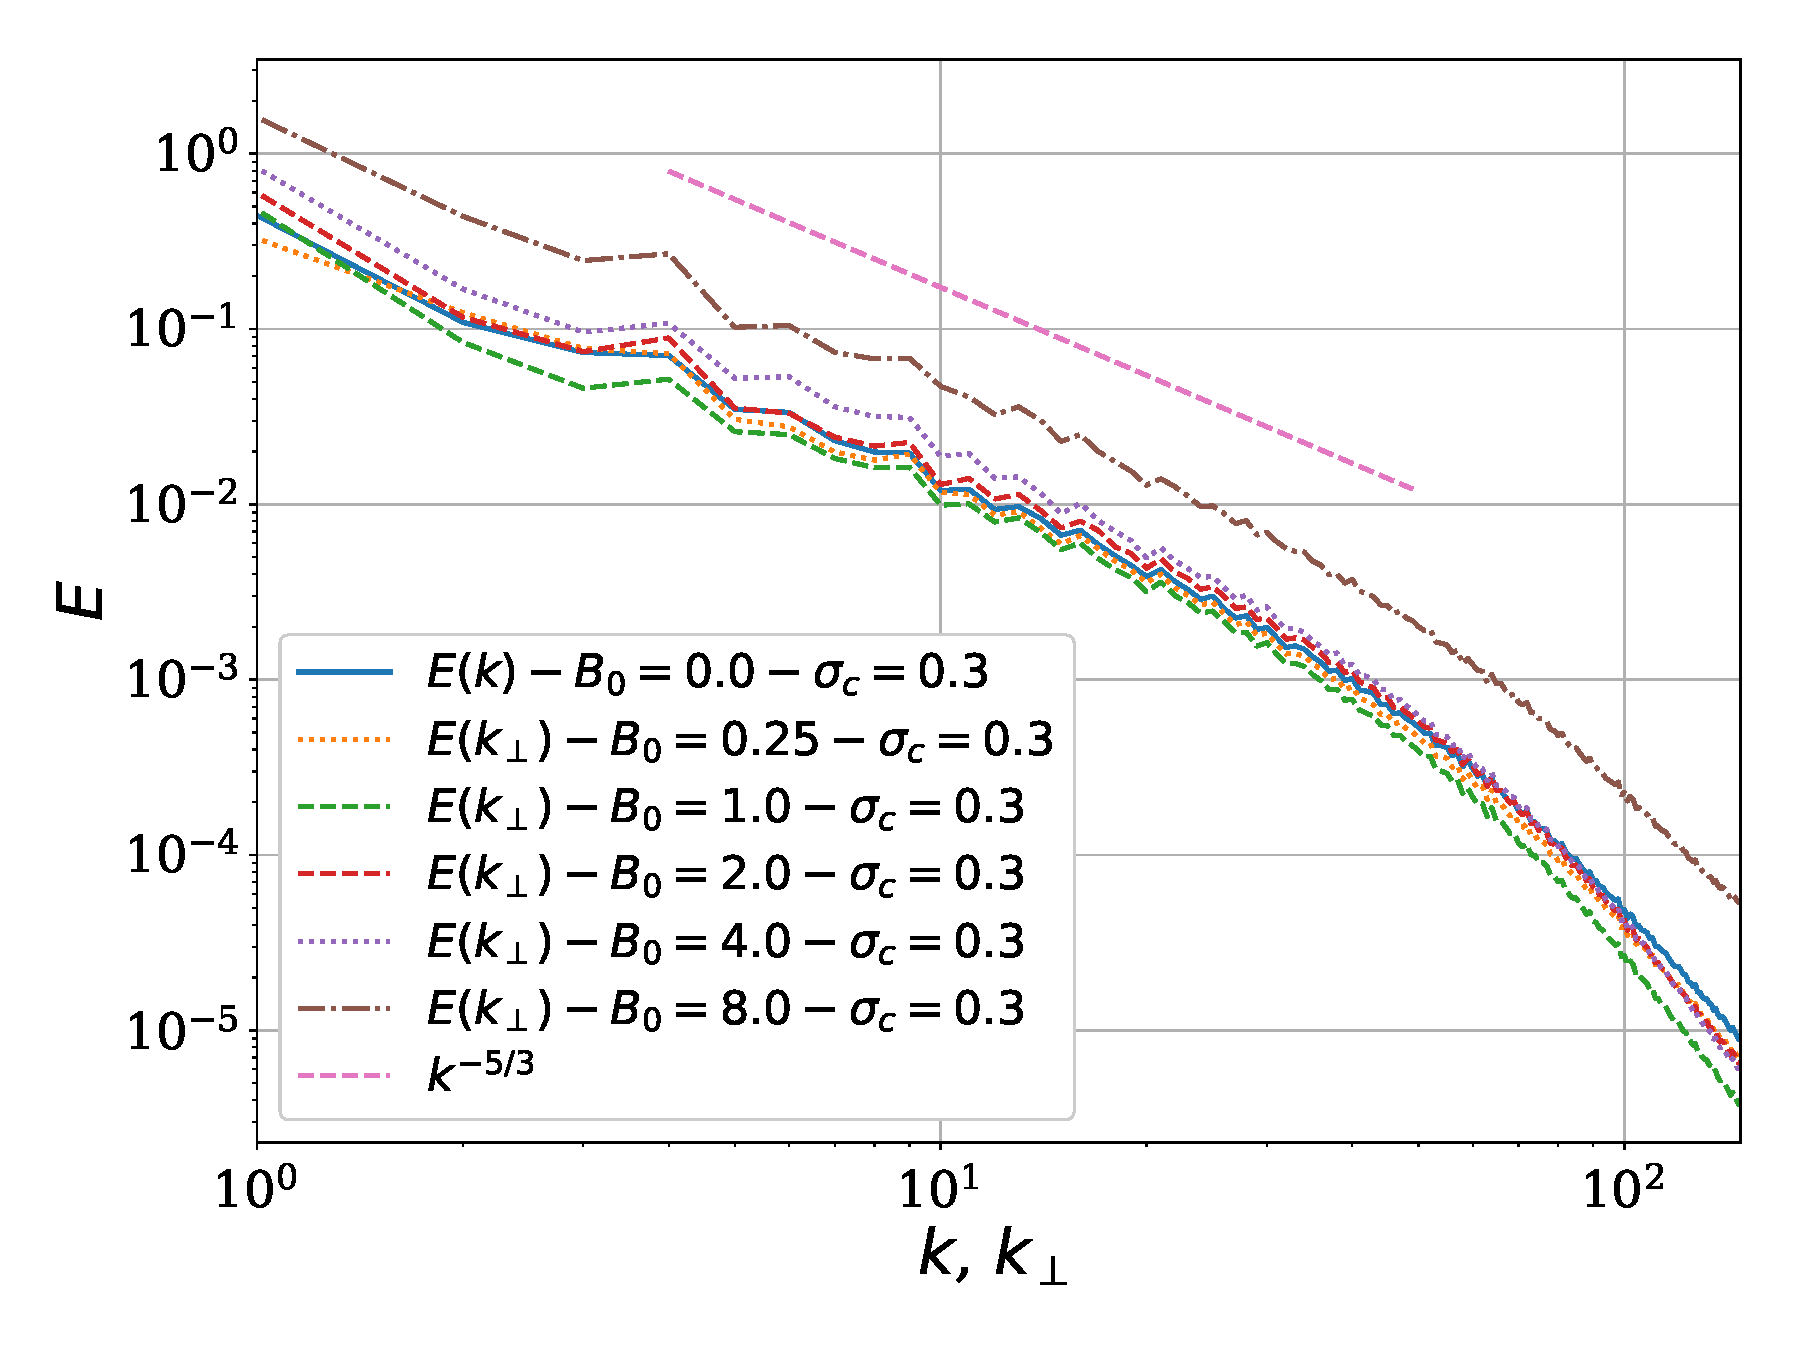
\includegraphics[width=1\columnwidth]{SpatioTemporalSpectra/fig1_E-eps-converted-to.pdf}
  \caption{Reduced perpendicular energy spectra $E(k_\perp)$ for the
    simulations with $B_0=0.25$, $1$, $4$, and $8$, and isotropic energy
    spectrum $E(k)$ for the simulation with $B_0=0$. Kolmogorov
    scaling, $\sim k_\perp^{-5/3}$, is shown as reference.}
  \label{fig1:E}
\end{figure}


La \cref{fig2:isocontourns} muestra los contornos de
$e(k_\perp,k_\parallel)/\sin(\theta_k)$, es decir, el espectro
axisimétrico (promediado temporalmente) para las corridas con $B_0=0$,
$B_0=1$, $B_0=4$ y $B_0=8$. Para el flujo isotrópico ($B_0=0$, ver
\cref{fig2:isocontourns}a), los contornos de
$e(k_\perp,k_\parallel)/\sin(\theta_k)$ son círculos, tal como se
esperaba \cite{mininni_isotropization_2012}.  A medida que la
intensidad del campo guía aumenta, la energía se comienza a concentrar
cerca del eje con$k_\parallel=0$, evidenciando la formación de
estructuras elongadas en la dirección del campo guía (o, en otras
palabras, del relativo decrecimiento de los gradientes paralelos del
campo con respecto a los gradientes perpendiculares).

Los tiempos característicos definidos en la sección \ref{sec_Wfspectrum_and_Gamma}, $\tau_A$,
$\tau_{sw}$, y $\tau_{nl}$, dividen el espacio de Fourier en la \cref{fig2:isocontourns} en regiones dependiendo de cómo se ordenan las escalas temporales:
\begin{equation}\label{eq:Asw} \tau_A < \tau_{sw} \hspace{0.05cm}
\Rightarrow \hspace{0.05cm} k_\perp <
\left(\sqrt{\left(\frac{B_0}{v_{rms}}\right)^2 \cdot
\left(\frac{C_{sw}}{C_A}\right)^2 - 1} \right) k_\parallel,
\end{equation}
\begin{equation}\label{eq:Anl} \tau_A < \tau_{nl} \hspace{0.05cm}
\Rightarrow \hspace{0.05cm} k_\perp <
\left(\sqrt{\left(\frac{B_0}{v_{rms}}\right)^3
\left(\frac{C_{nl}}{C_A}\right)^3 Lk_\parallel - 1} \right) 
k_\parallel,
\end{equation}
\begin{equation}\label{eq:nlsw} \tau_{nl} < \tau_{sw} \hspace{0.05cm}
\Rightarrow \hspace{0.05cm} \left( k_\perp^2 + k_\parallel^2
\right)^{1/6} < \frac{C_{sw}}{C_{nl}L^{1/3}}.
\end{equation}
En la \cref{fig2:isocontourns} también se indican las curvas
correspondientes a los modos que satisfacen las relaciones
$\tau_A\lesssim\tau_{sw}$ y $\tau_A\lesssim\tau_{nl}$, para $B_0=1$,
$4$ y $8$ (asumiento, para dibujar las curvas, que $C_{sw} \approx
C_{nl} \approx C_A \approx 1$; esta elección fue posteriormente
confirmada por el análisis de las funciones de correlación). Debe
mencionarse que la curva $\tau_A\approx\tau_{nl}$ también cumple un
rol muy importante en la teoría de balances críticos
\cite{sridhar_toward_1994}.

Como puede verse de la \cref{eq:nlsw}, la región donde
$\tau_{nl}\leq\tau_{sw}$ es un círculo pequeño alrededor del origen,
donde $k_\perp^2 + k_\parallel^2 \leq (C_{sw}/L^{1/3}C_{nl})^6 \approx
1$, y no se puede ver en la figura. Los modos fuera de la región con
$\tau_{nl}<\tau_{sw}$ deberían descorrelacionarse con el tiempo de
\textit{sweeping} o con el tiempo de Alfvén, dependiendo de cuál sea
más rápido. La \cref{eq:Asw} nos dice que en el área a la izquierda de
la curva $\tau_A\sim\tau_{sw}$ tenemos $\tau_A<\tau_{sw}$, mientras
que la \cref{eq:Anl} nos dice que en el área a la izquierda de la
curva $\tau_A\sim\tau_{nl}$ tenemos $\tau_A<\tau_{nl}$ (ver
\cref{fig2:isocontourns}b). Para el valor más grande de $B_0$
considerado (i.e., la simulación con $B_0=8$), la mayoría de los modos
tienen al periodo de Alfvén como el tiempo más rápido (i.e., la mayor
área en el gráfico se encuentre arriba y a la izquierda de la curva
$\tau_A \sim \tau_{sw}$), a pesar de que una fracción significativa de
la energía en el sistema no esté en estos modos, sino que se
concentran cerca del eje con $k_\parallel = 0$.

\begin{figure*}
  \centering
%  \subfigure[$B_0=0$]{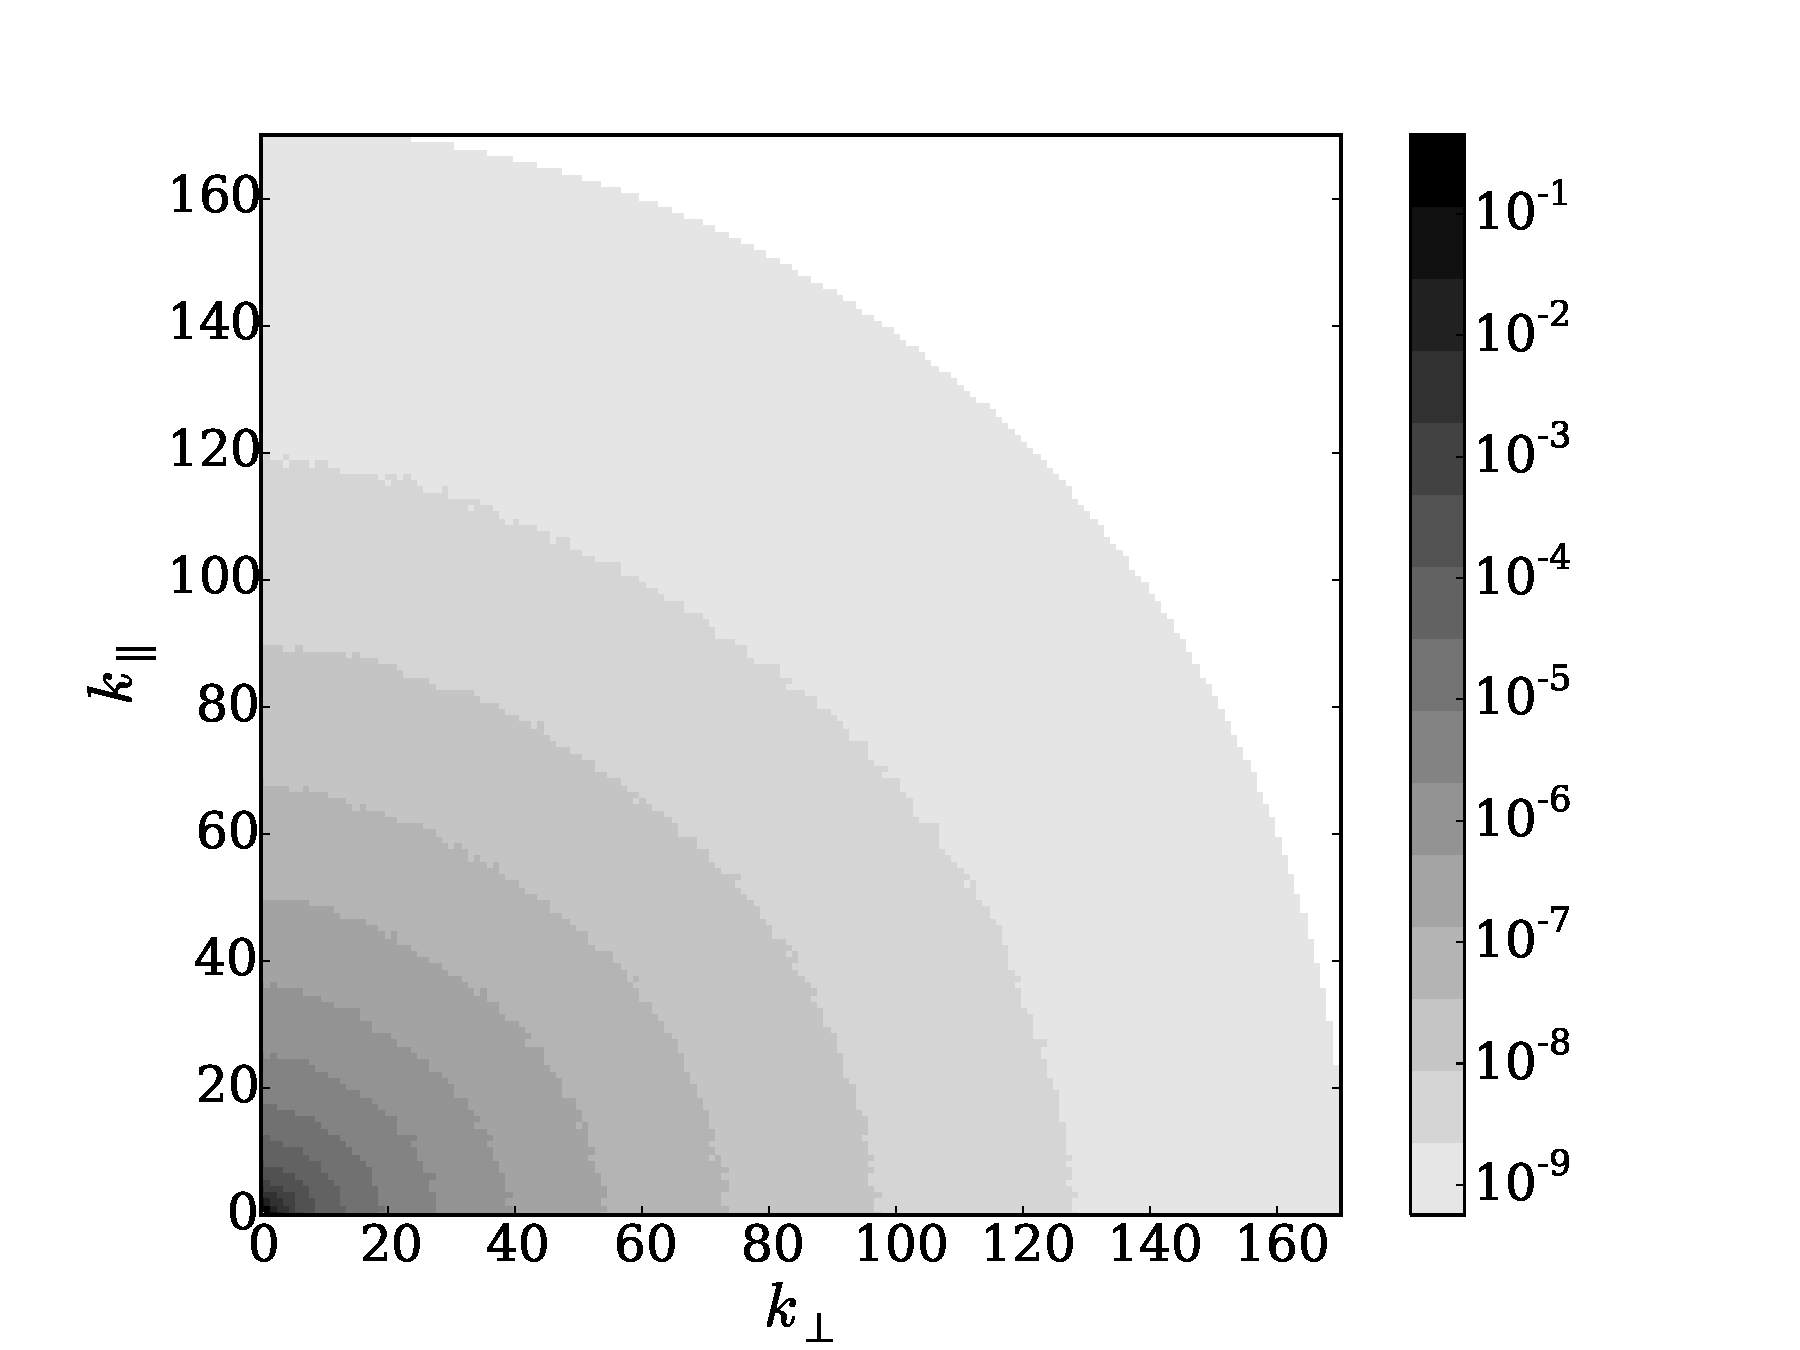
\includegraphics[width=0.45\textwidth]{SpatioTemporalSpectra/fig2_B0-eps-converted-to.pdf}}
%  \subfigure[$B_0=0.25$]{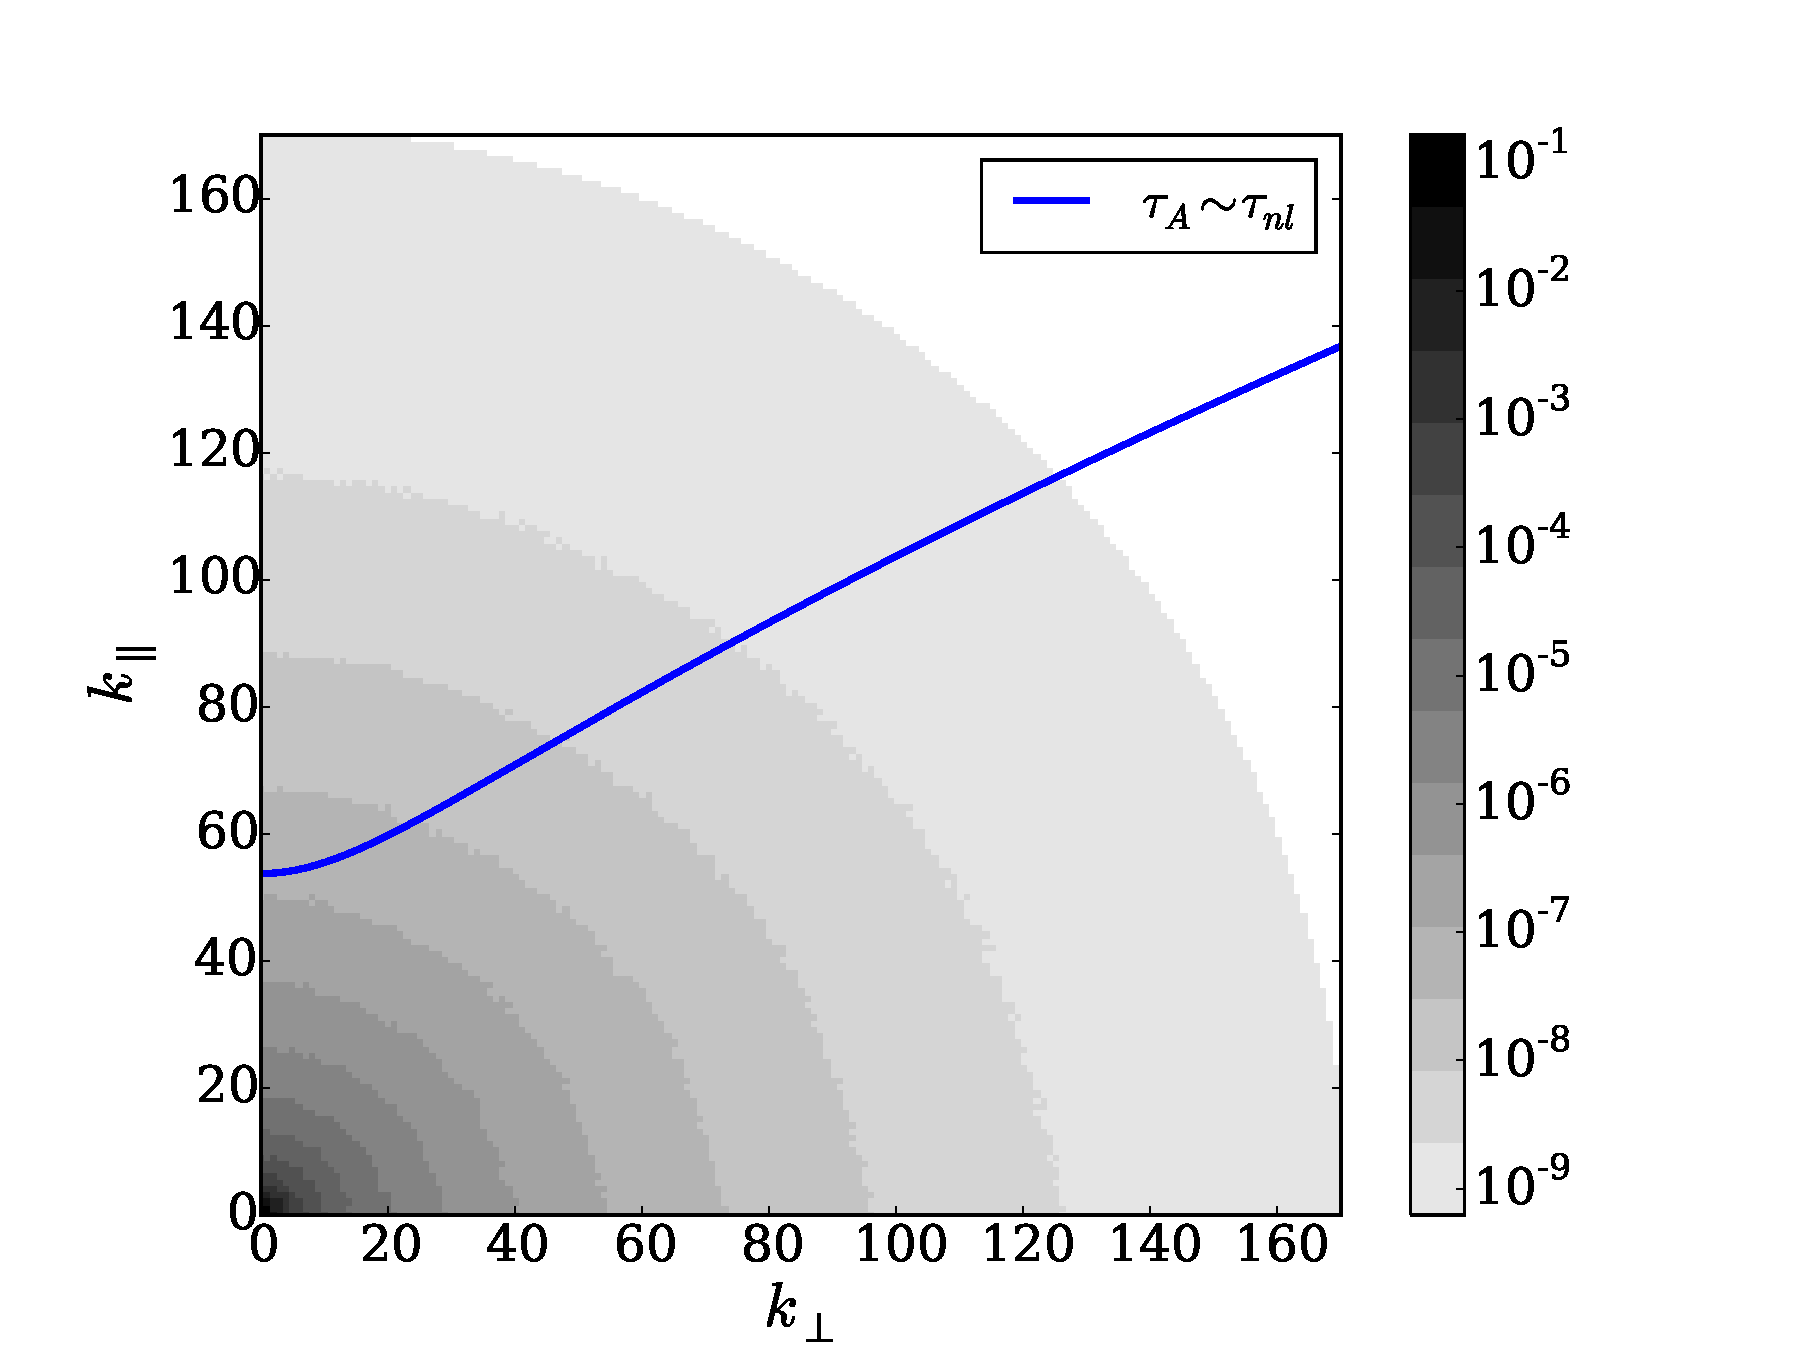
\includegraphics[width=0.45\textwidth]{SpatioTemporalSpectra/fig2_B025-eps-converted-to.pdf}}

%  \subfigure[$B_0=1$]{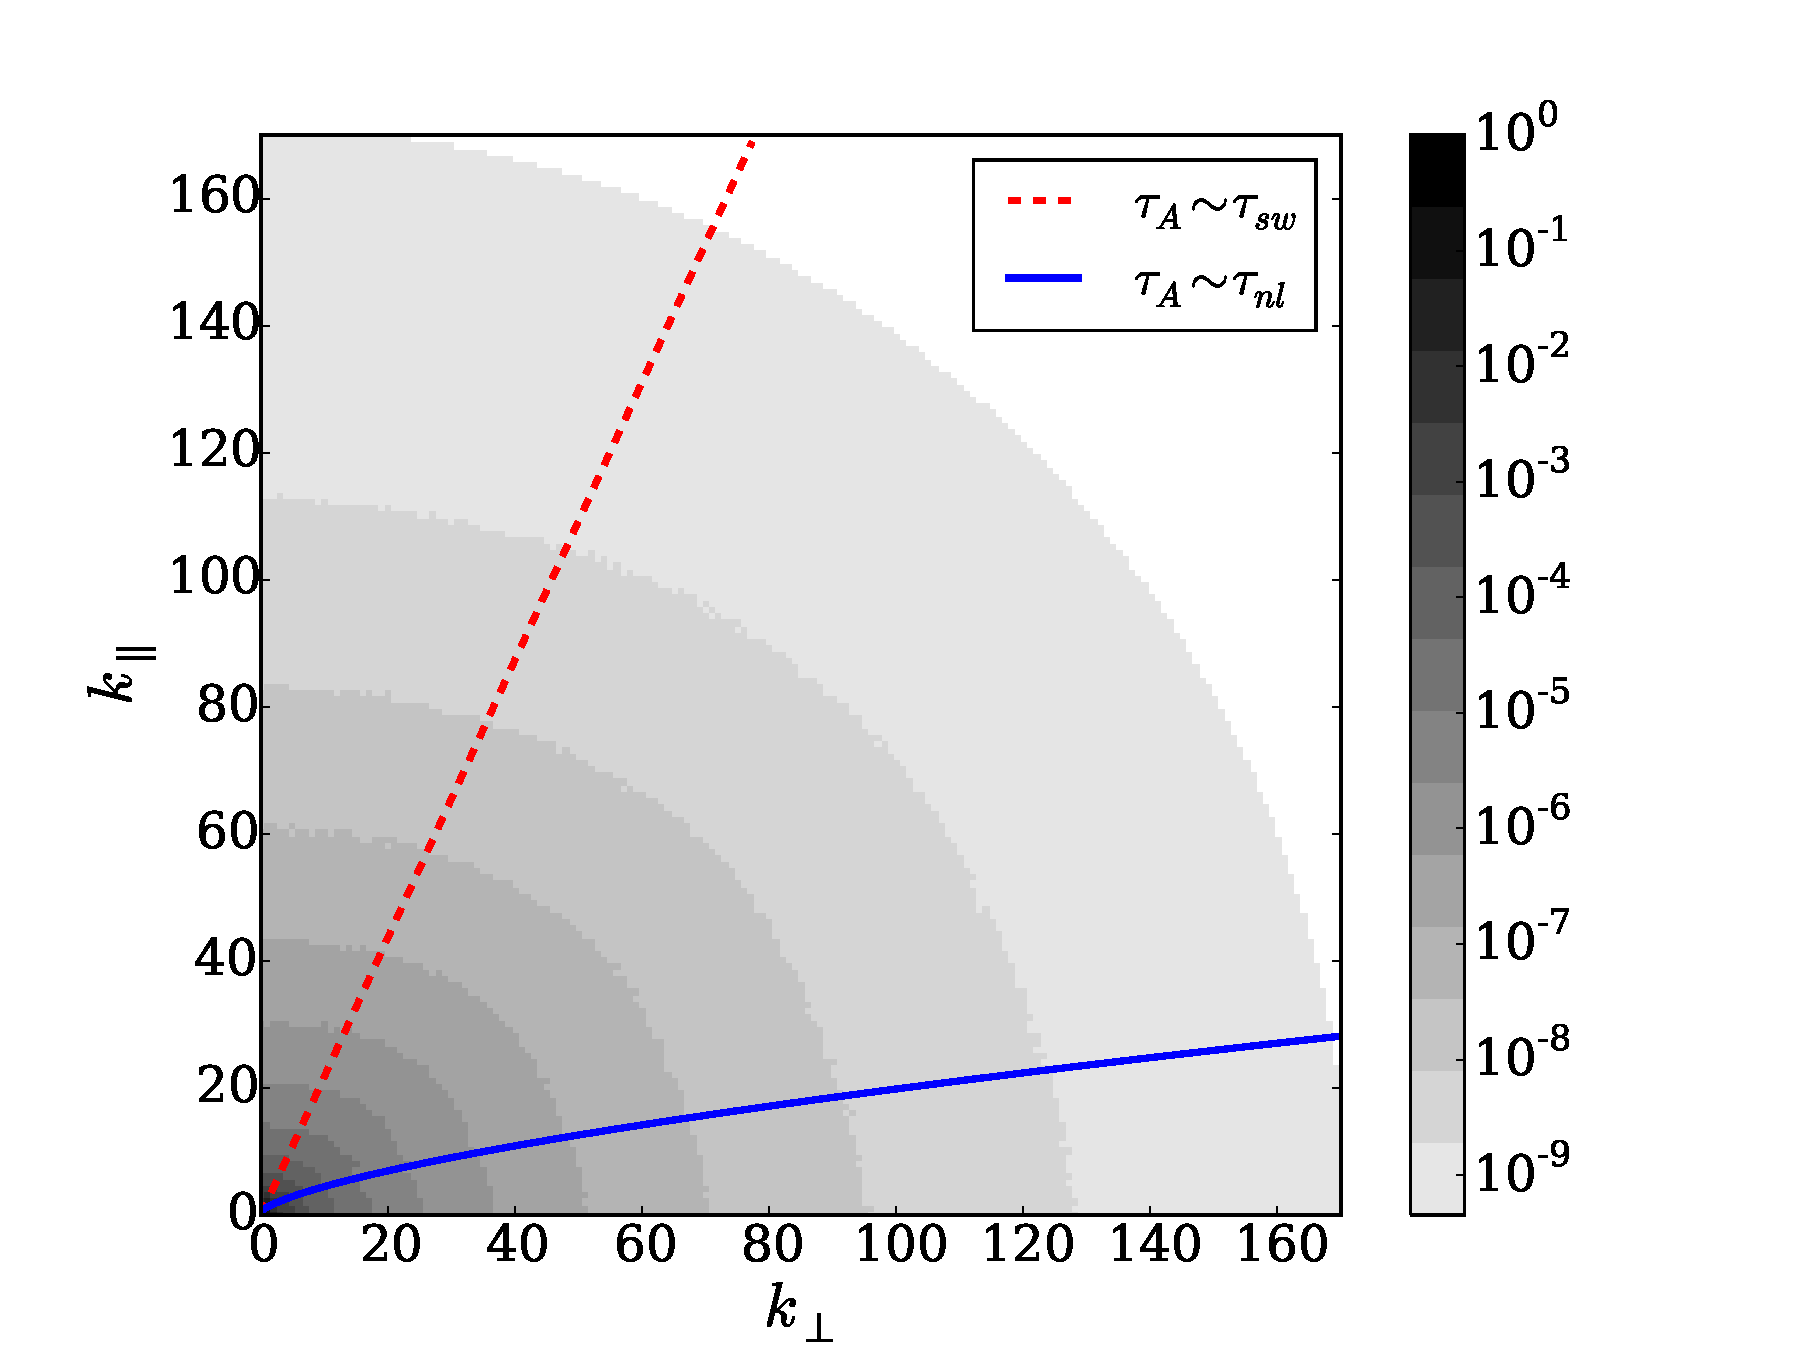
\includegraphics[width=0.45\textwidth]{SpatioTemporalSpectra/fig2_B1-eps-converted-to.pdf}}
%  \subfigure[$B_0=1$ with explanation]{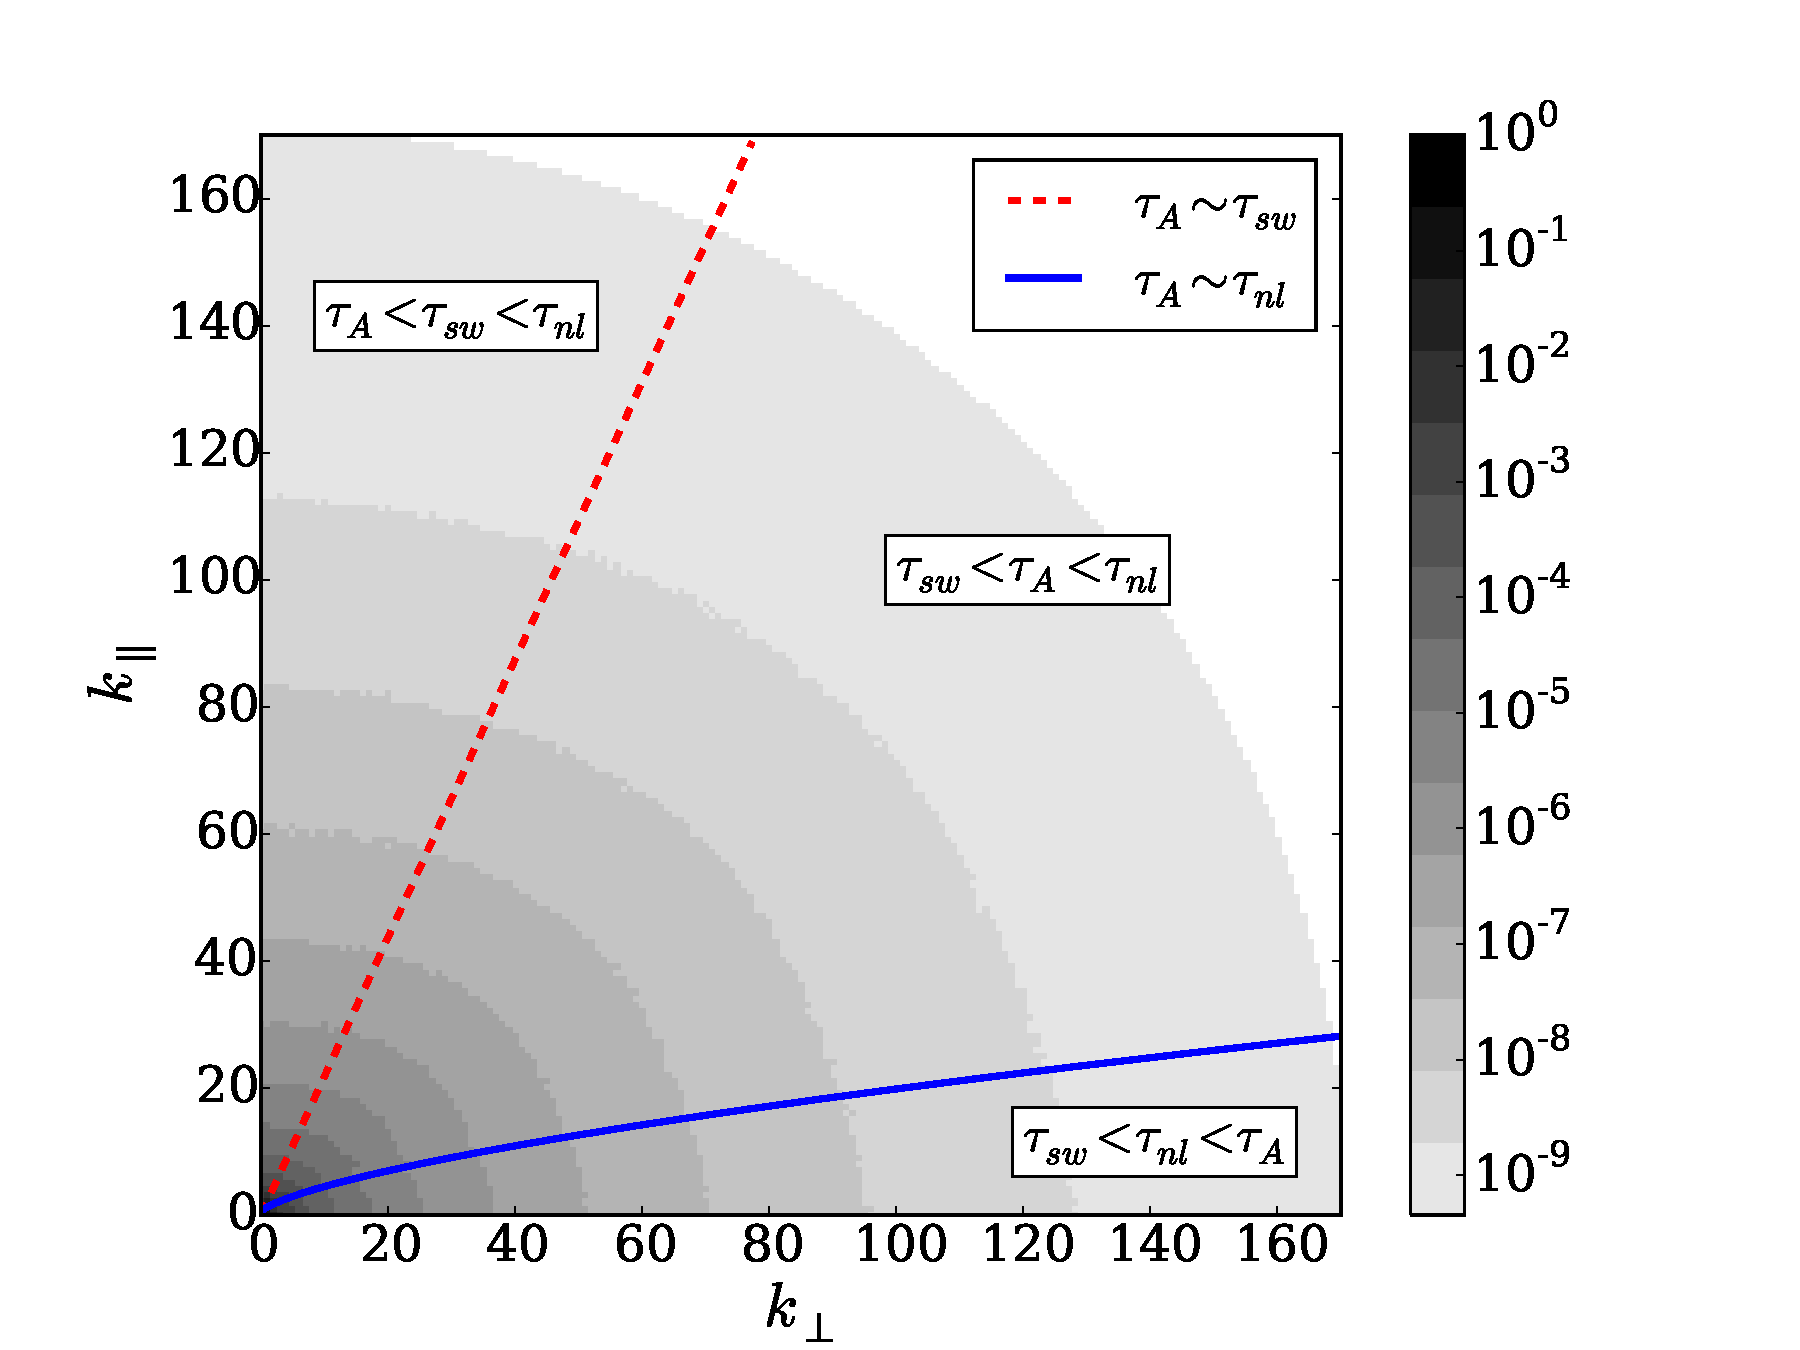
\includegraphics[width=0.45\textwidth]{SpatioTemporalSpectra/fig2_B1_explanation-eps-converted-to.pdf}}

%  \subfigure[$B_0=4$]{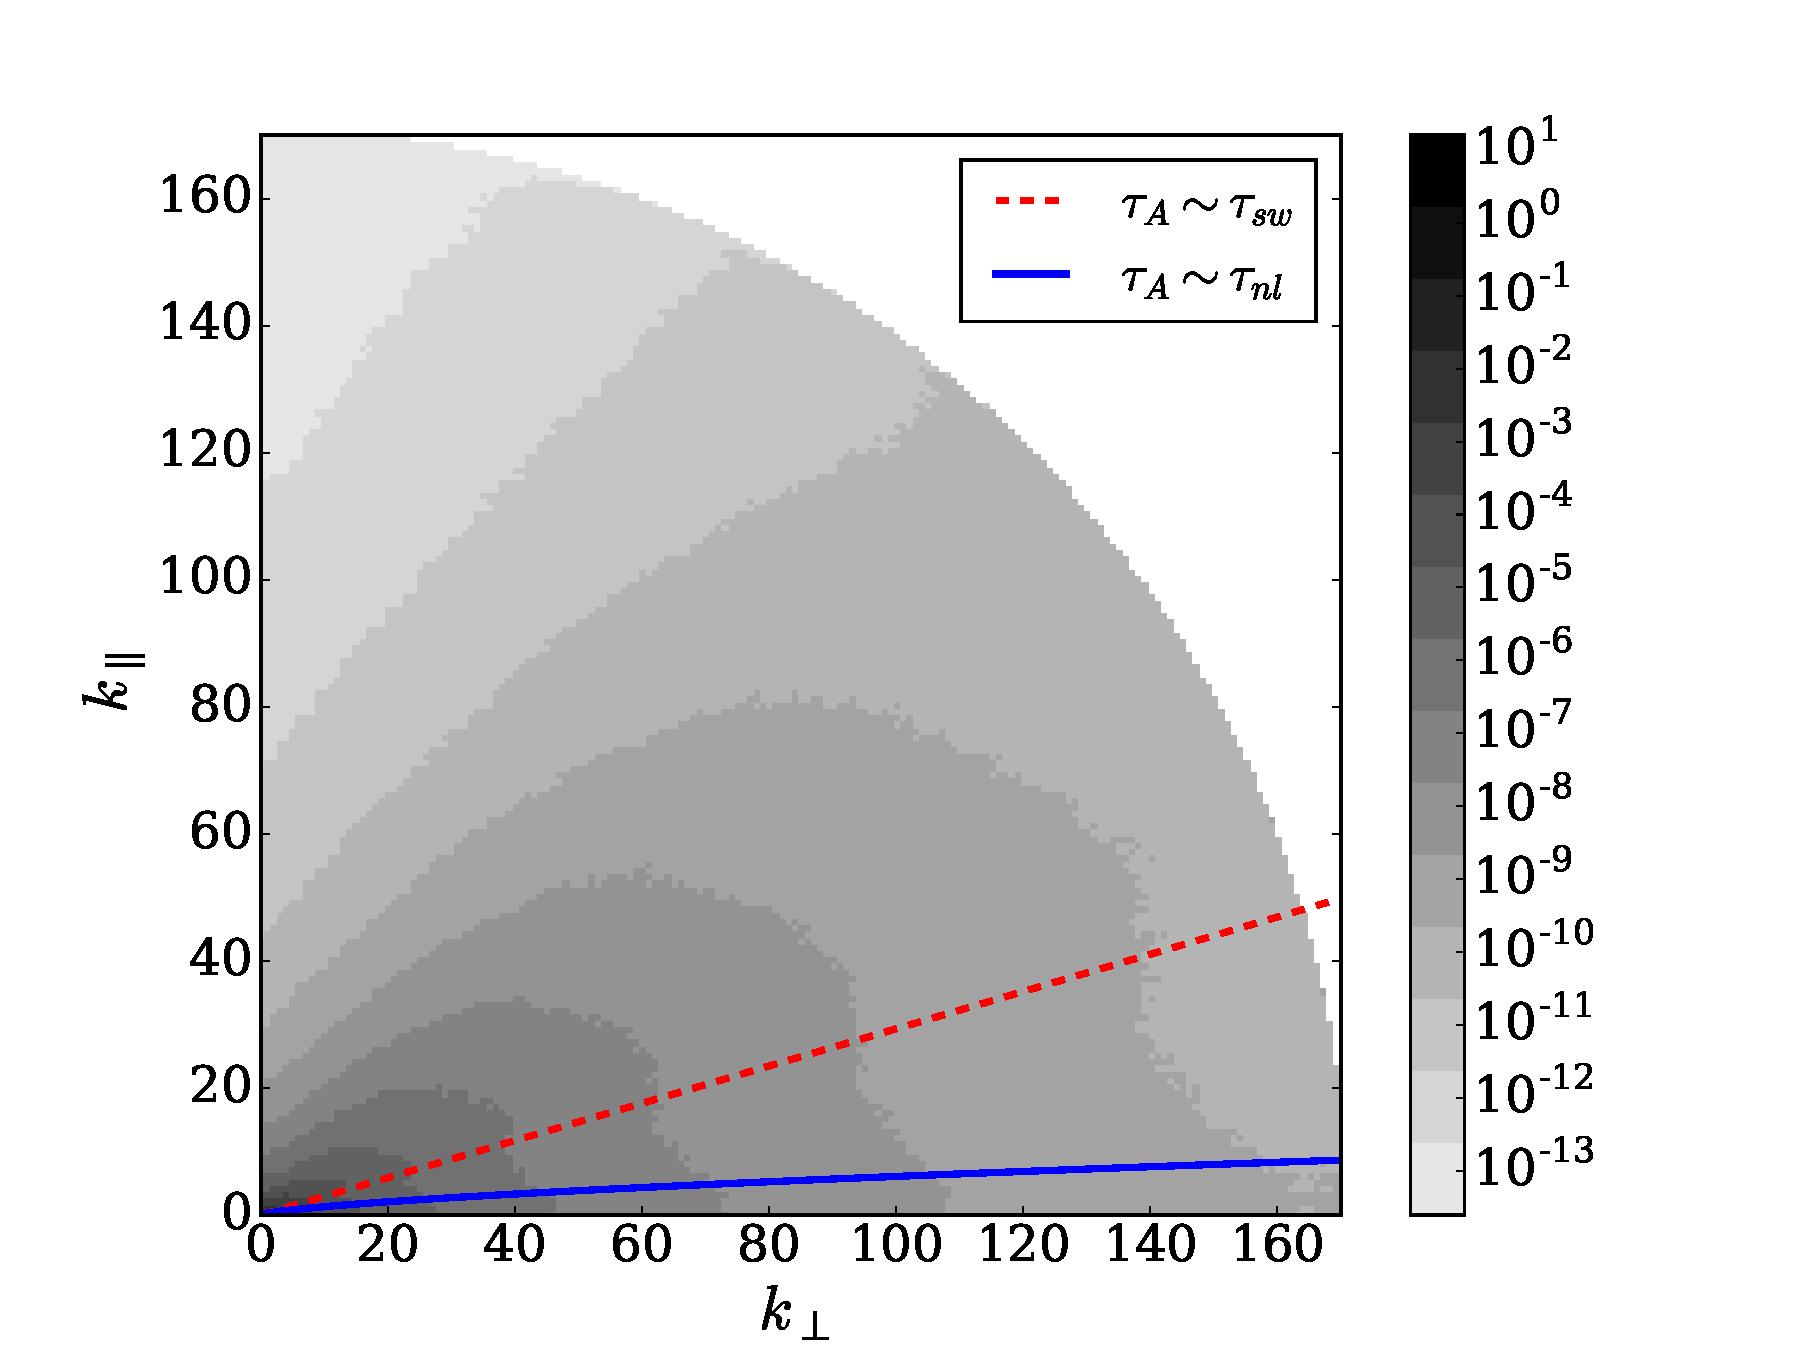
\includegraphics[width=0.45\textwidth]{SpatioTemporalSpectra/fig2_B4-eps-converted-to.pdf}}
%  \subfigure[$B_0=8$]{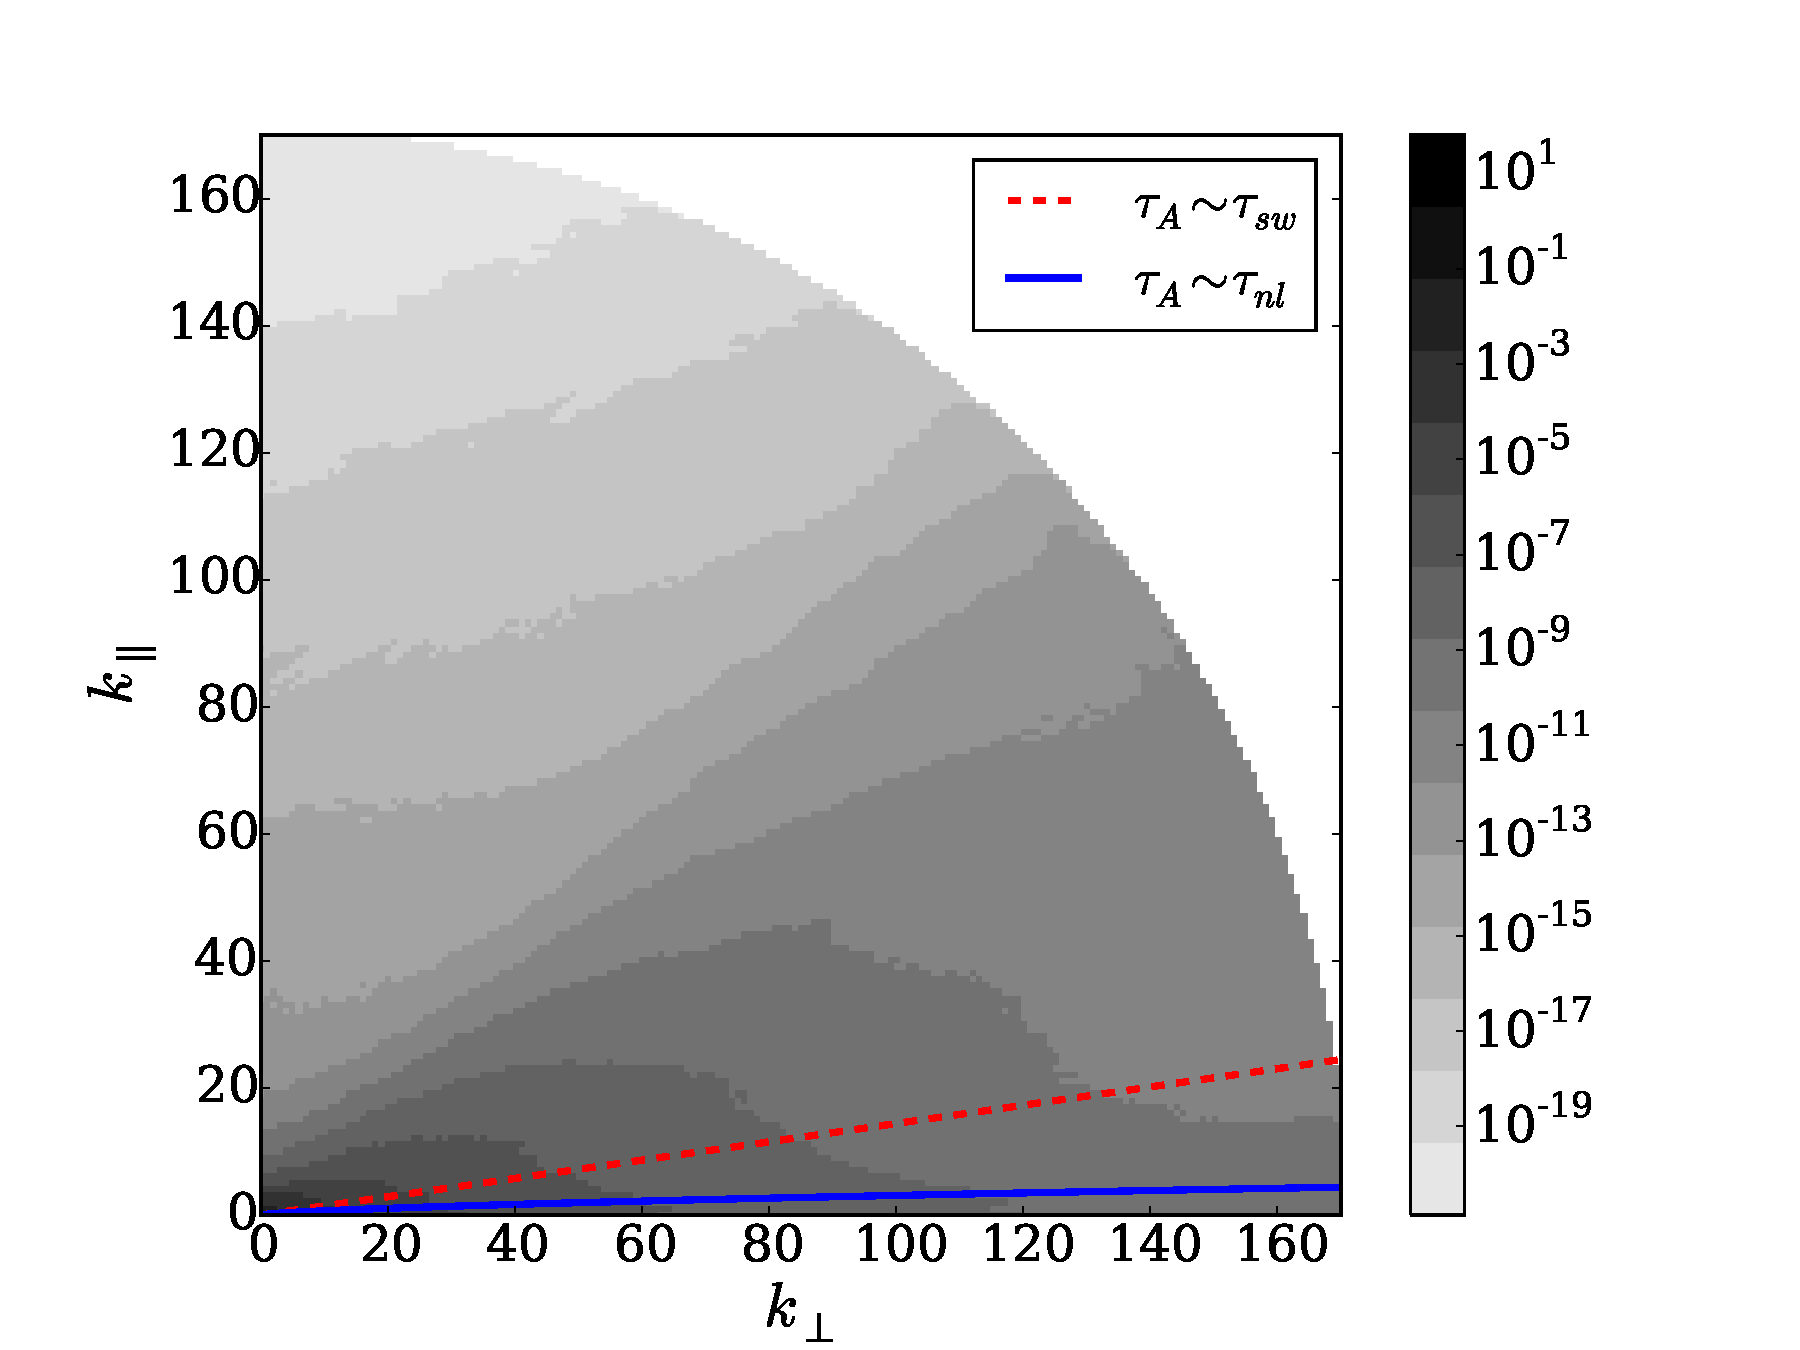
\includegraphics[width=0.45\textwidth]{SpatioTemporalSpectra/fig2_B8-eps-converted-to.pdf}}
  \subfigure[$B_0=0$]{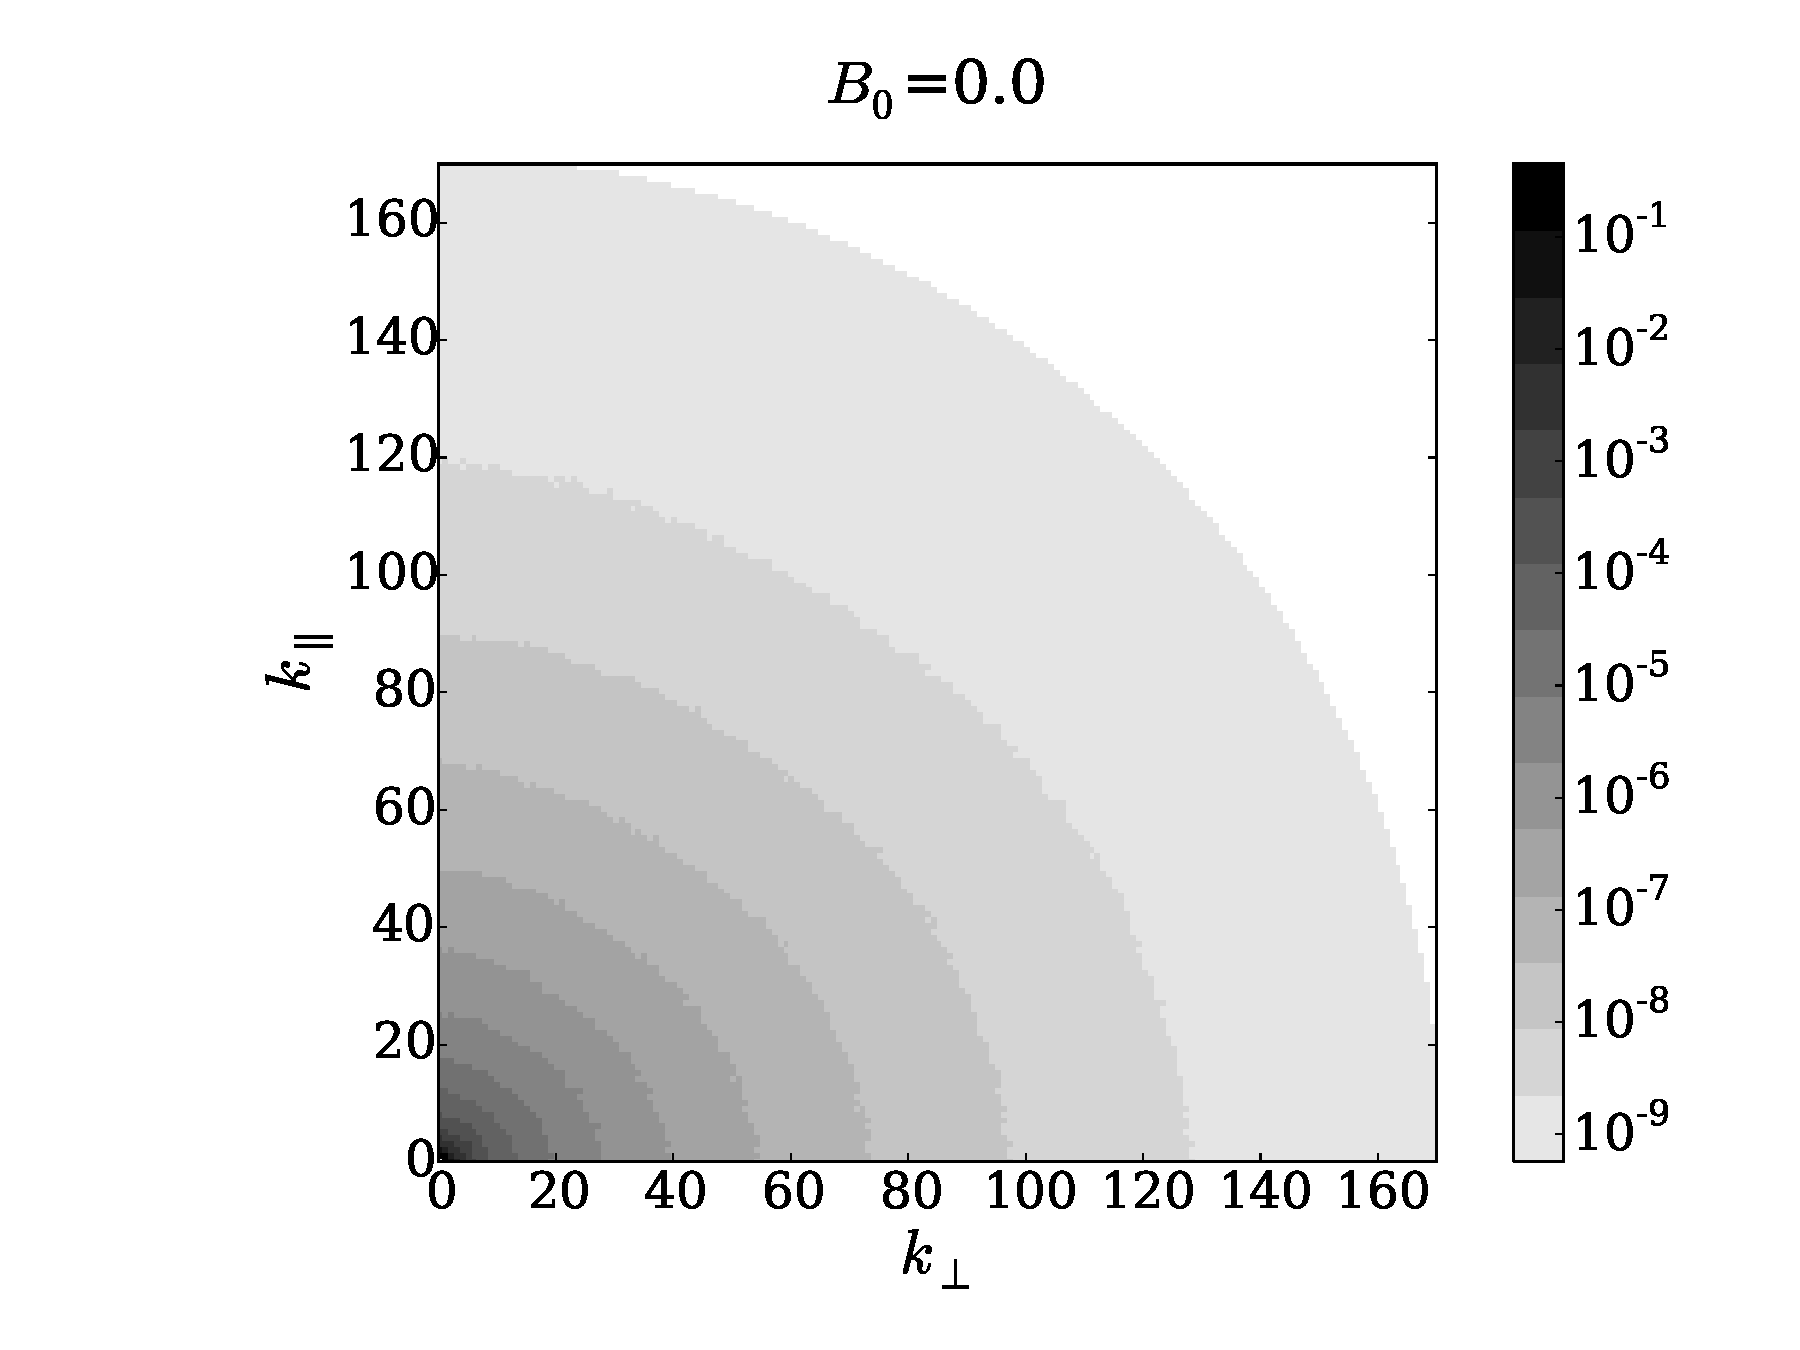
\includegraphics[width=0.48\textwidth]{SpatioTemporalSpectra/fig2_B0.pdf}}
  \subfigure[$B_0=1$]{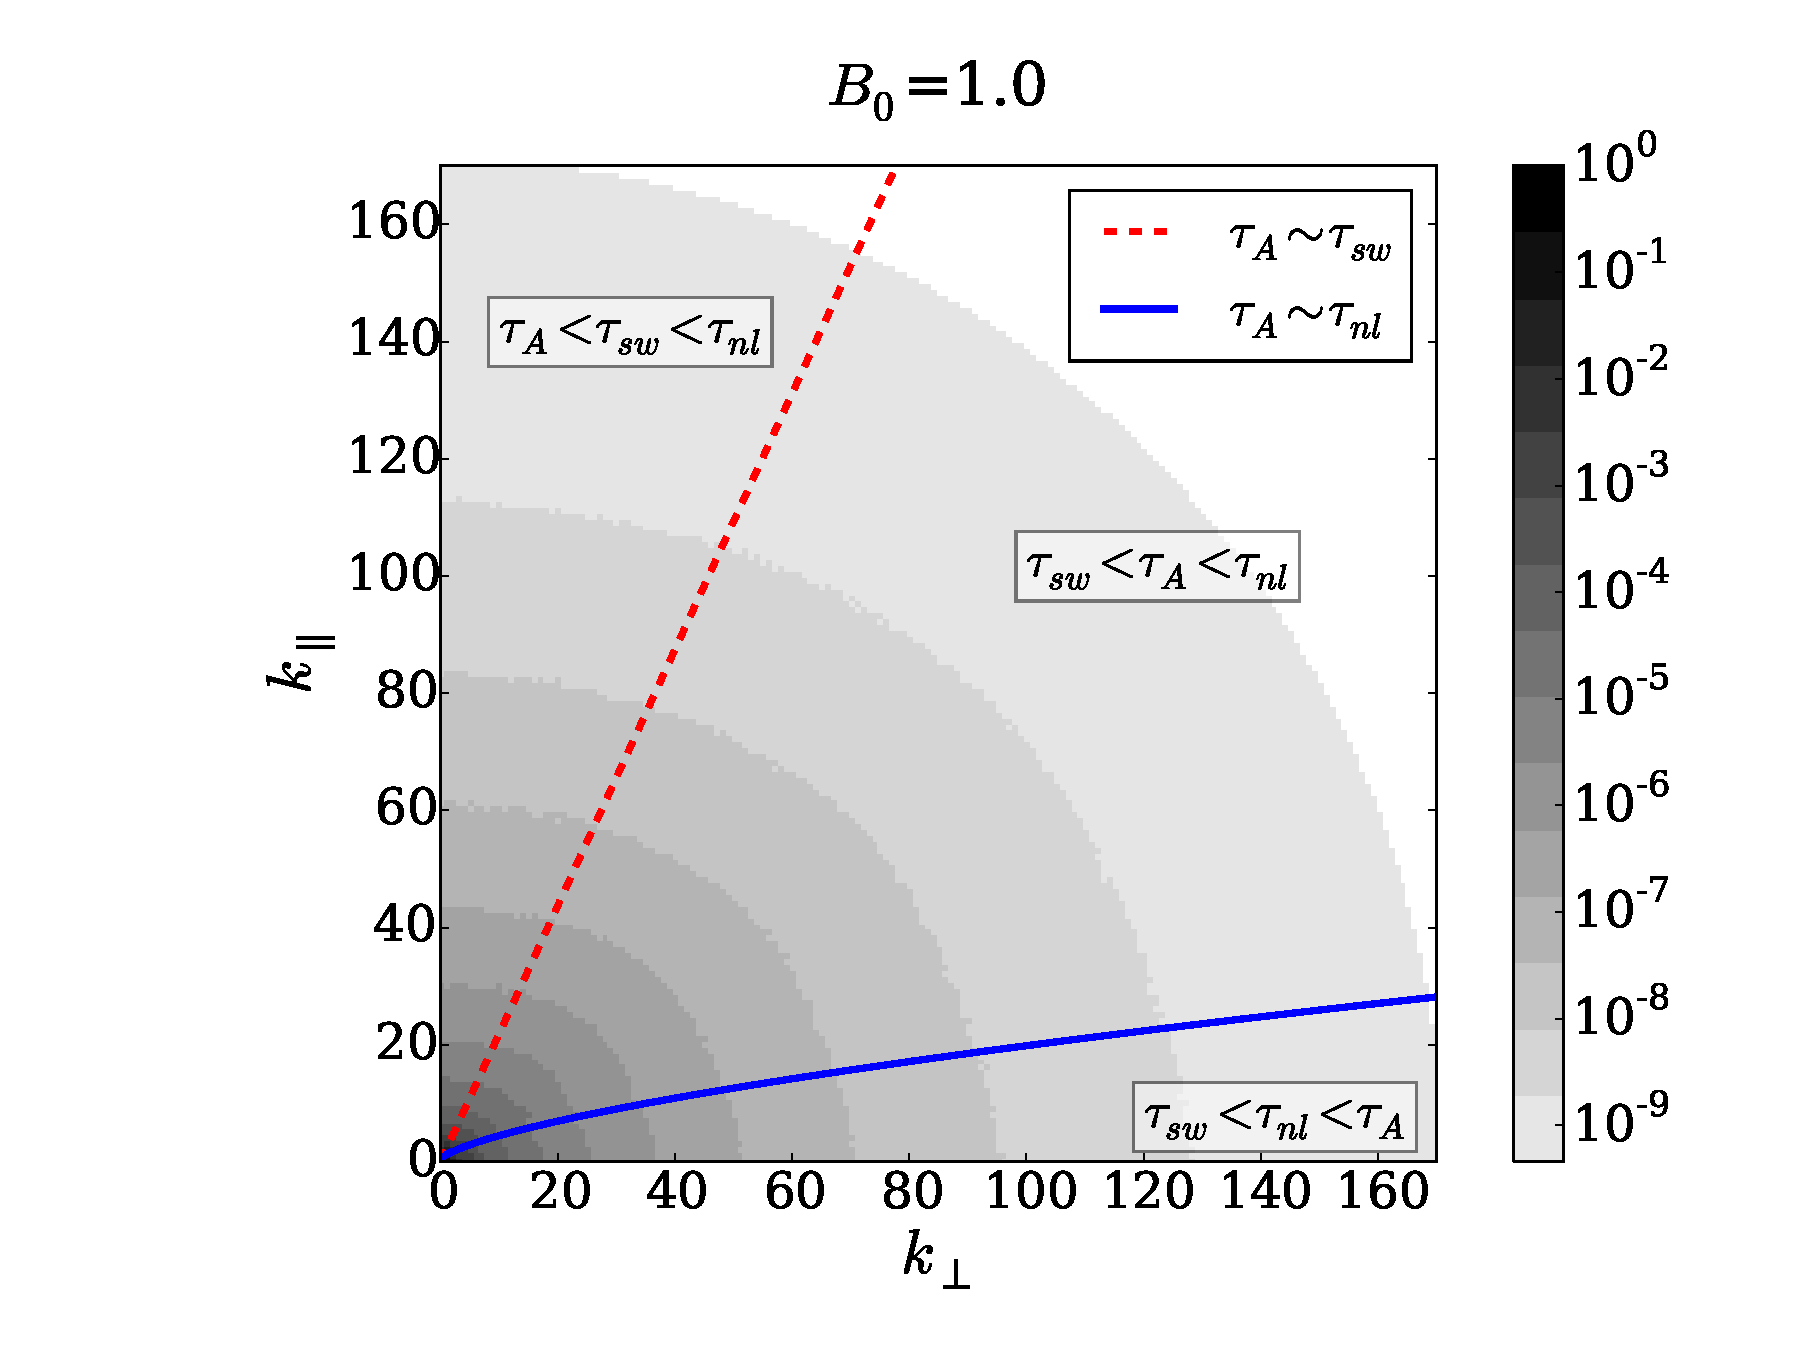
\includegraphics[width=0.48\textwidth]{SpatioTemporalSpectra/fig2_B1.pdf}}

  \subfigure[$B_0=4$]{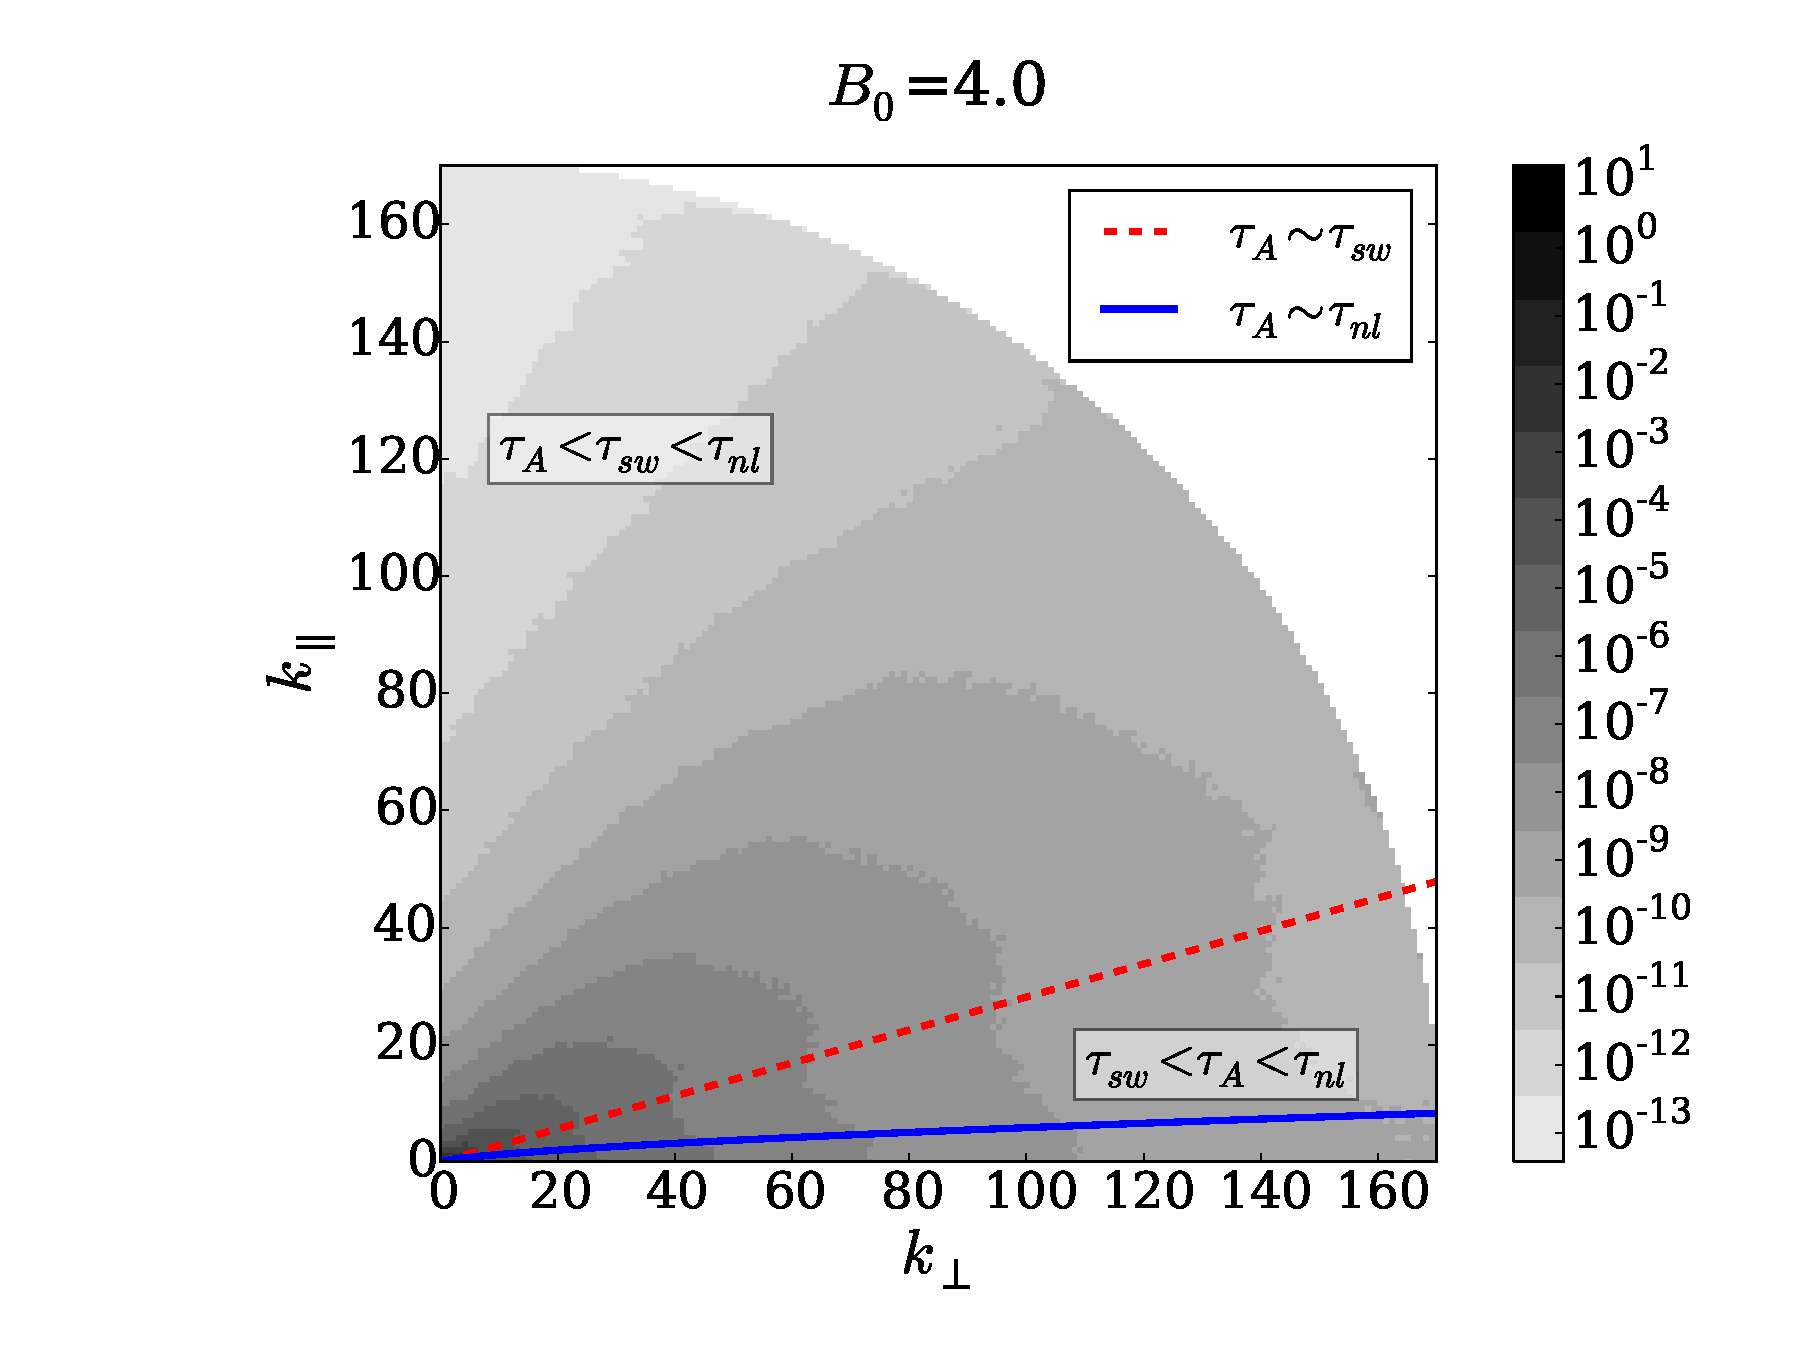
\includegraphics[width=0.48\textwidth]{SpatioTemporalSpectra/fig2_B4.pdf}}
  \subfigure[$B_0=4$ in log-log scale]{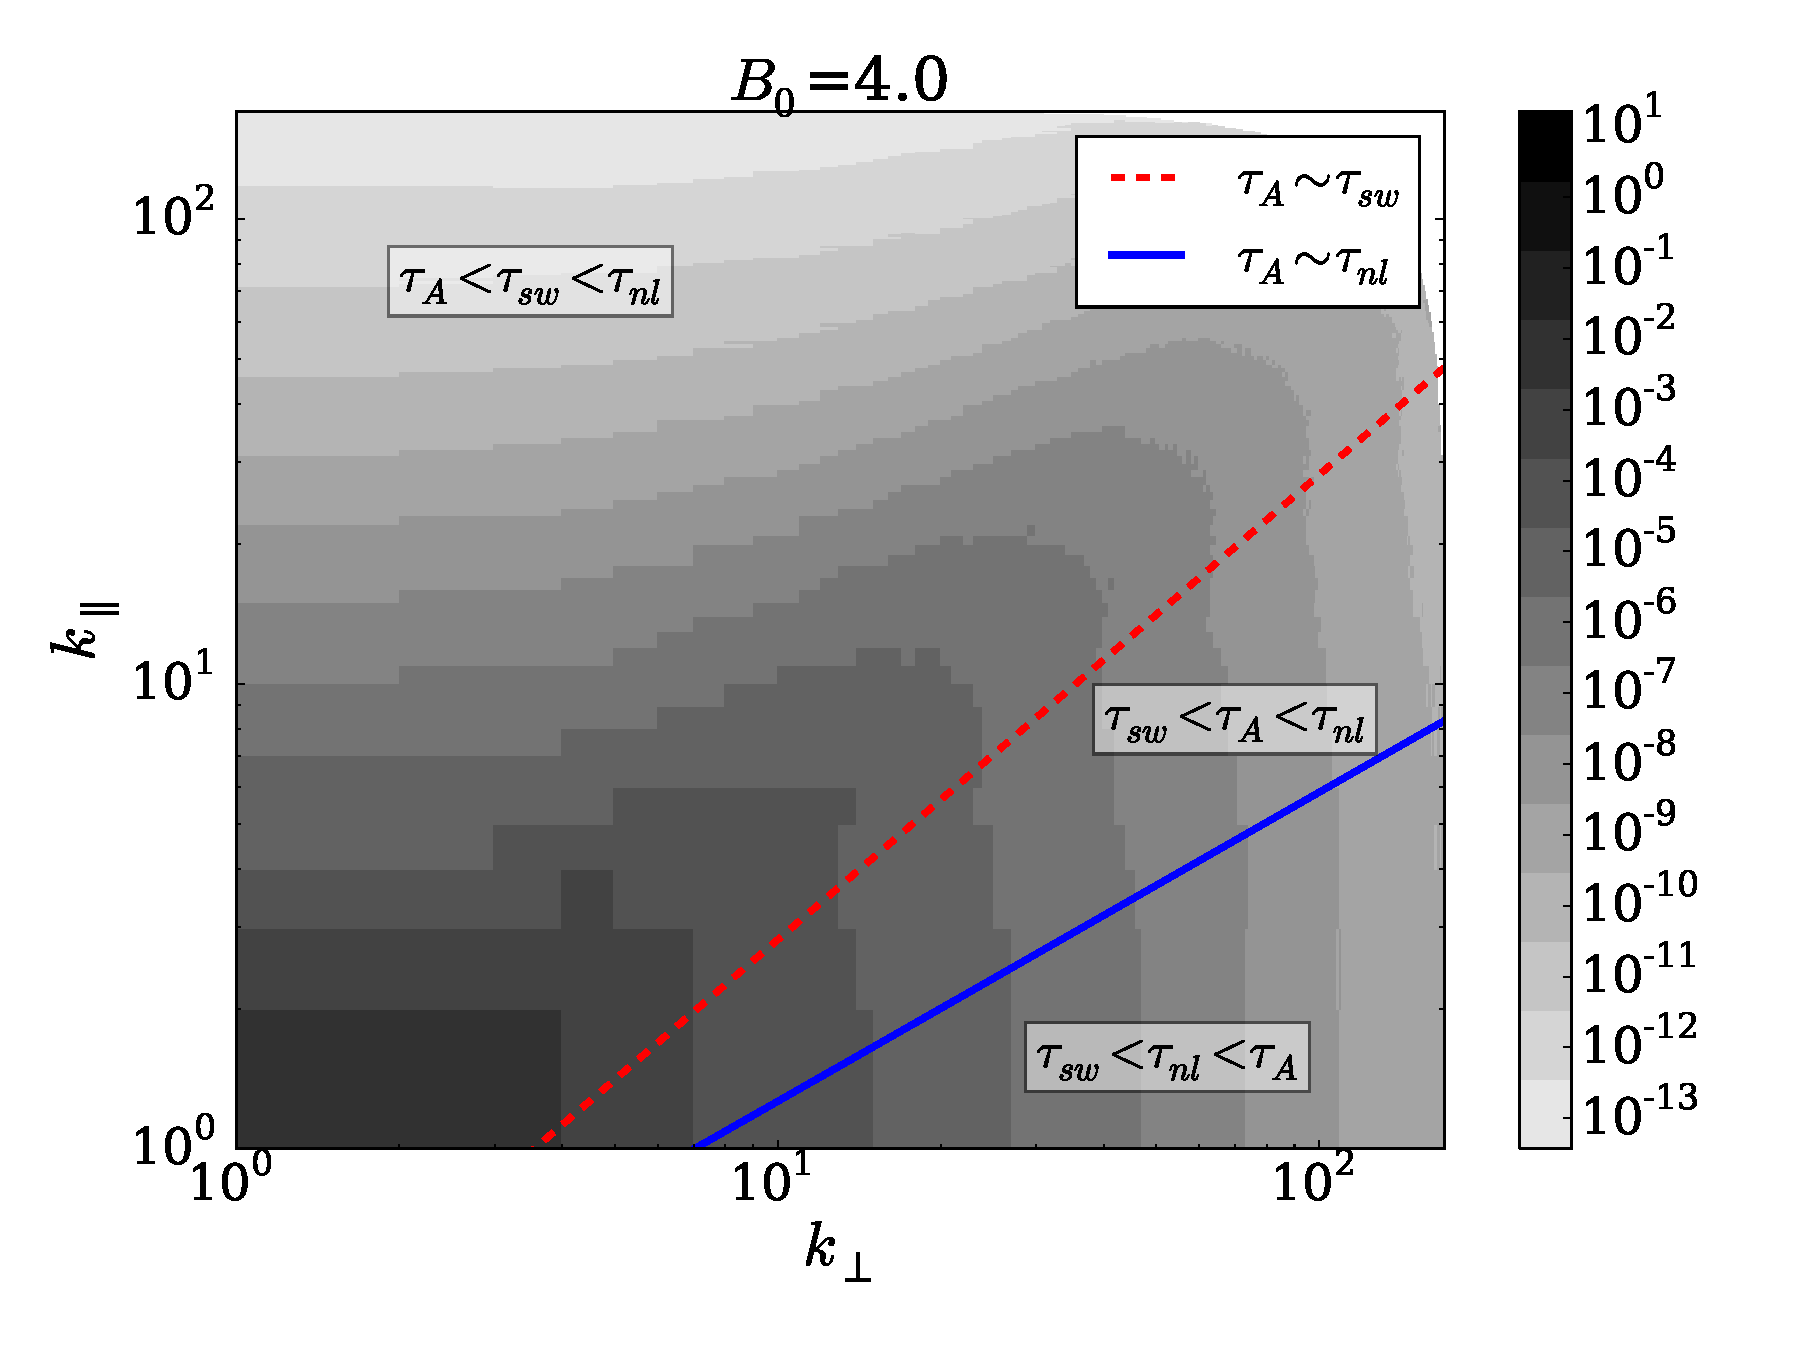
\includegraphics[width=0.48\textwidth]{SpatioTemporalSpectra/fig2_B4_log.pdf}}
%  \subfigure[$B_0=4$ in log-log scale]{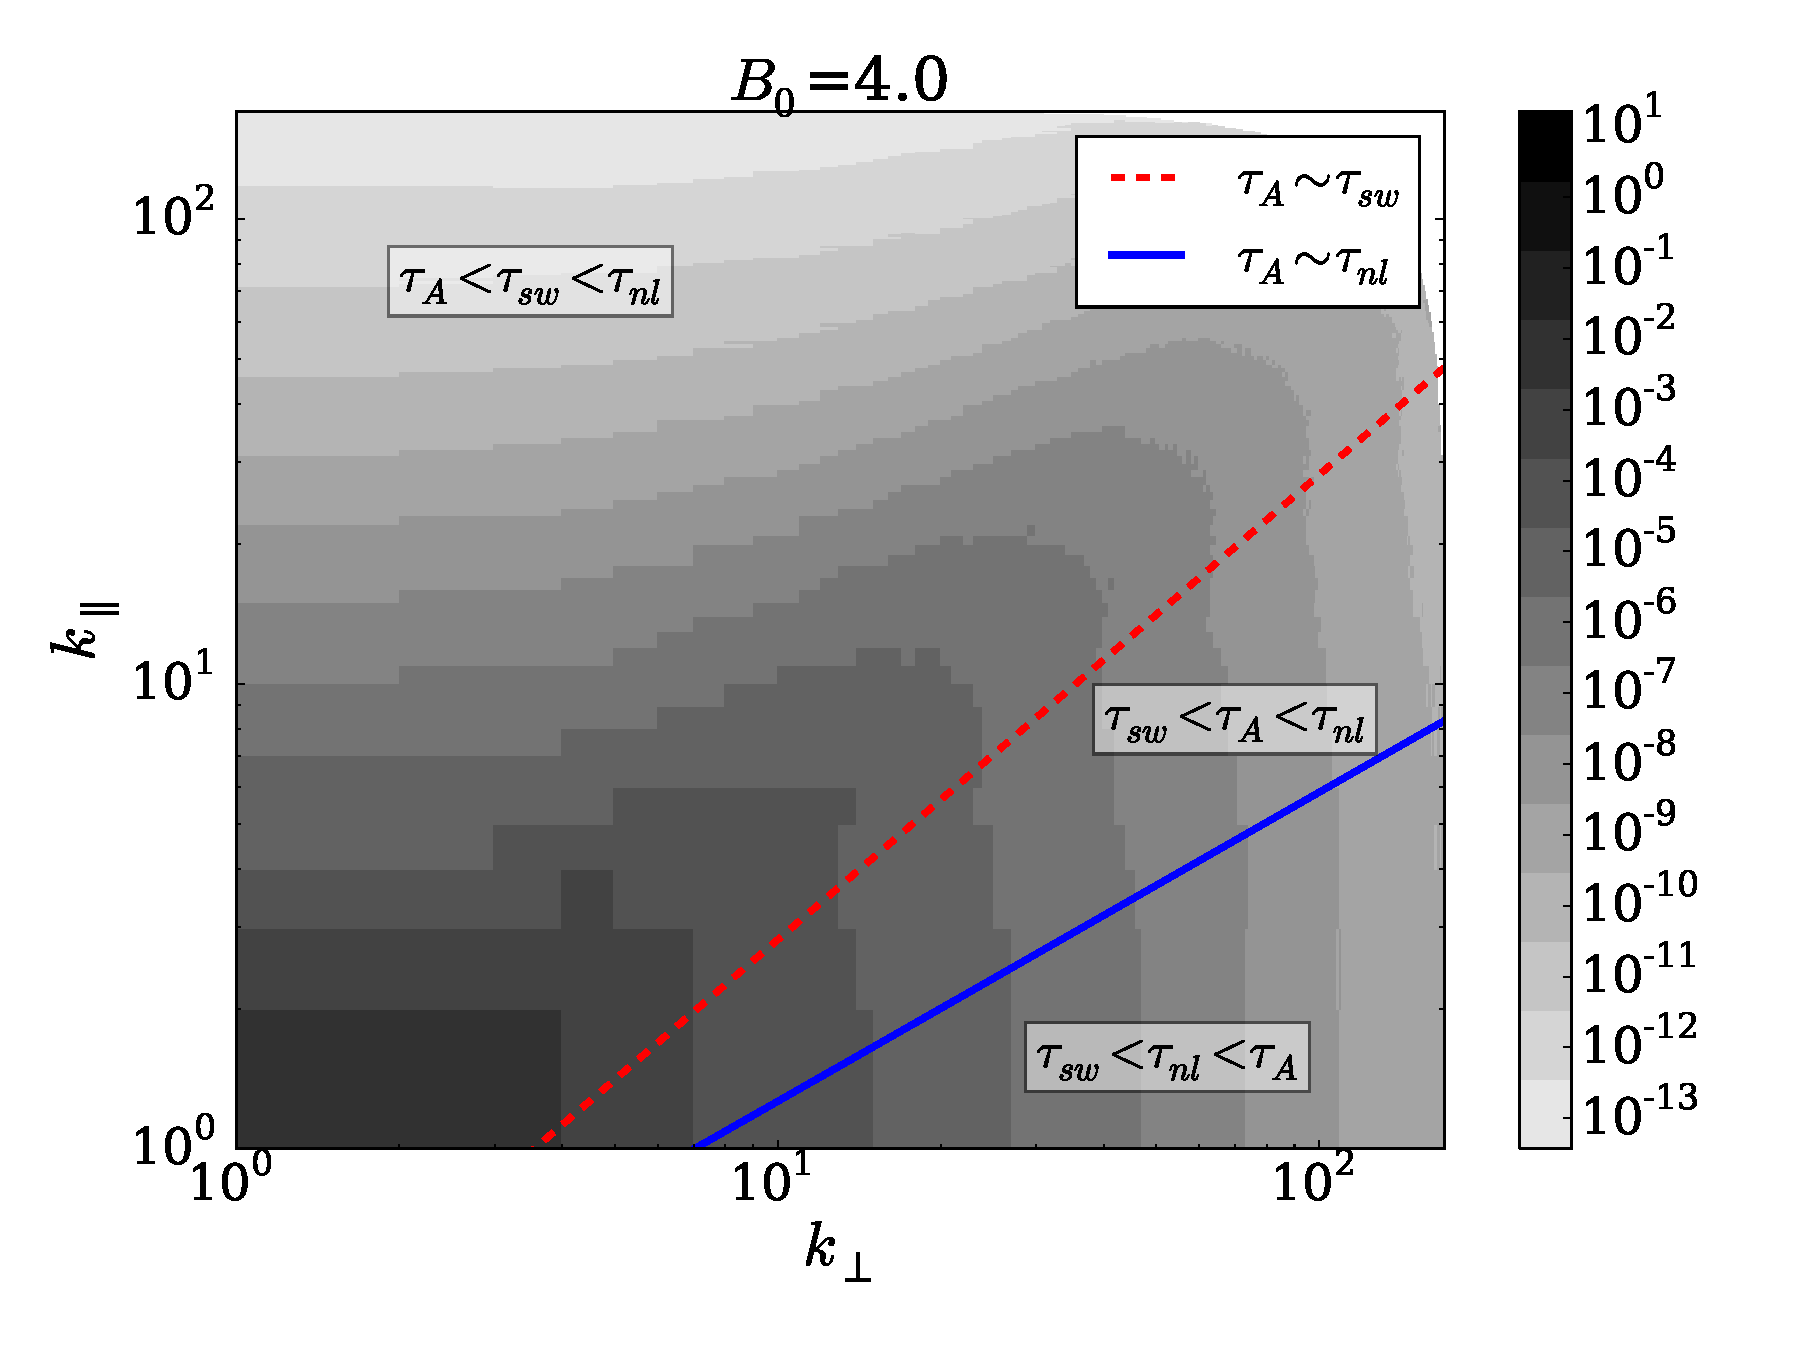
\includegraphics[width=0.45\textwidth]{SpatioTemporalSpectra/fig2_B4_log.eps}}

  \subfigure[$B_0=8$]{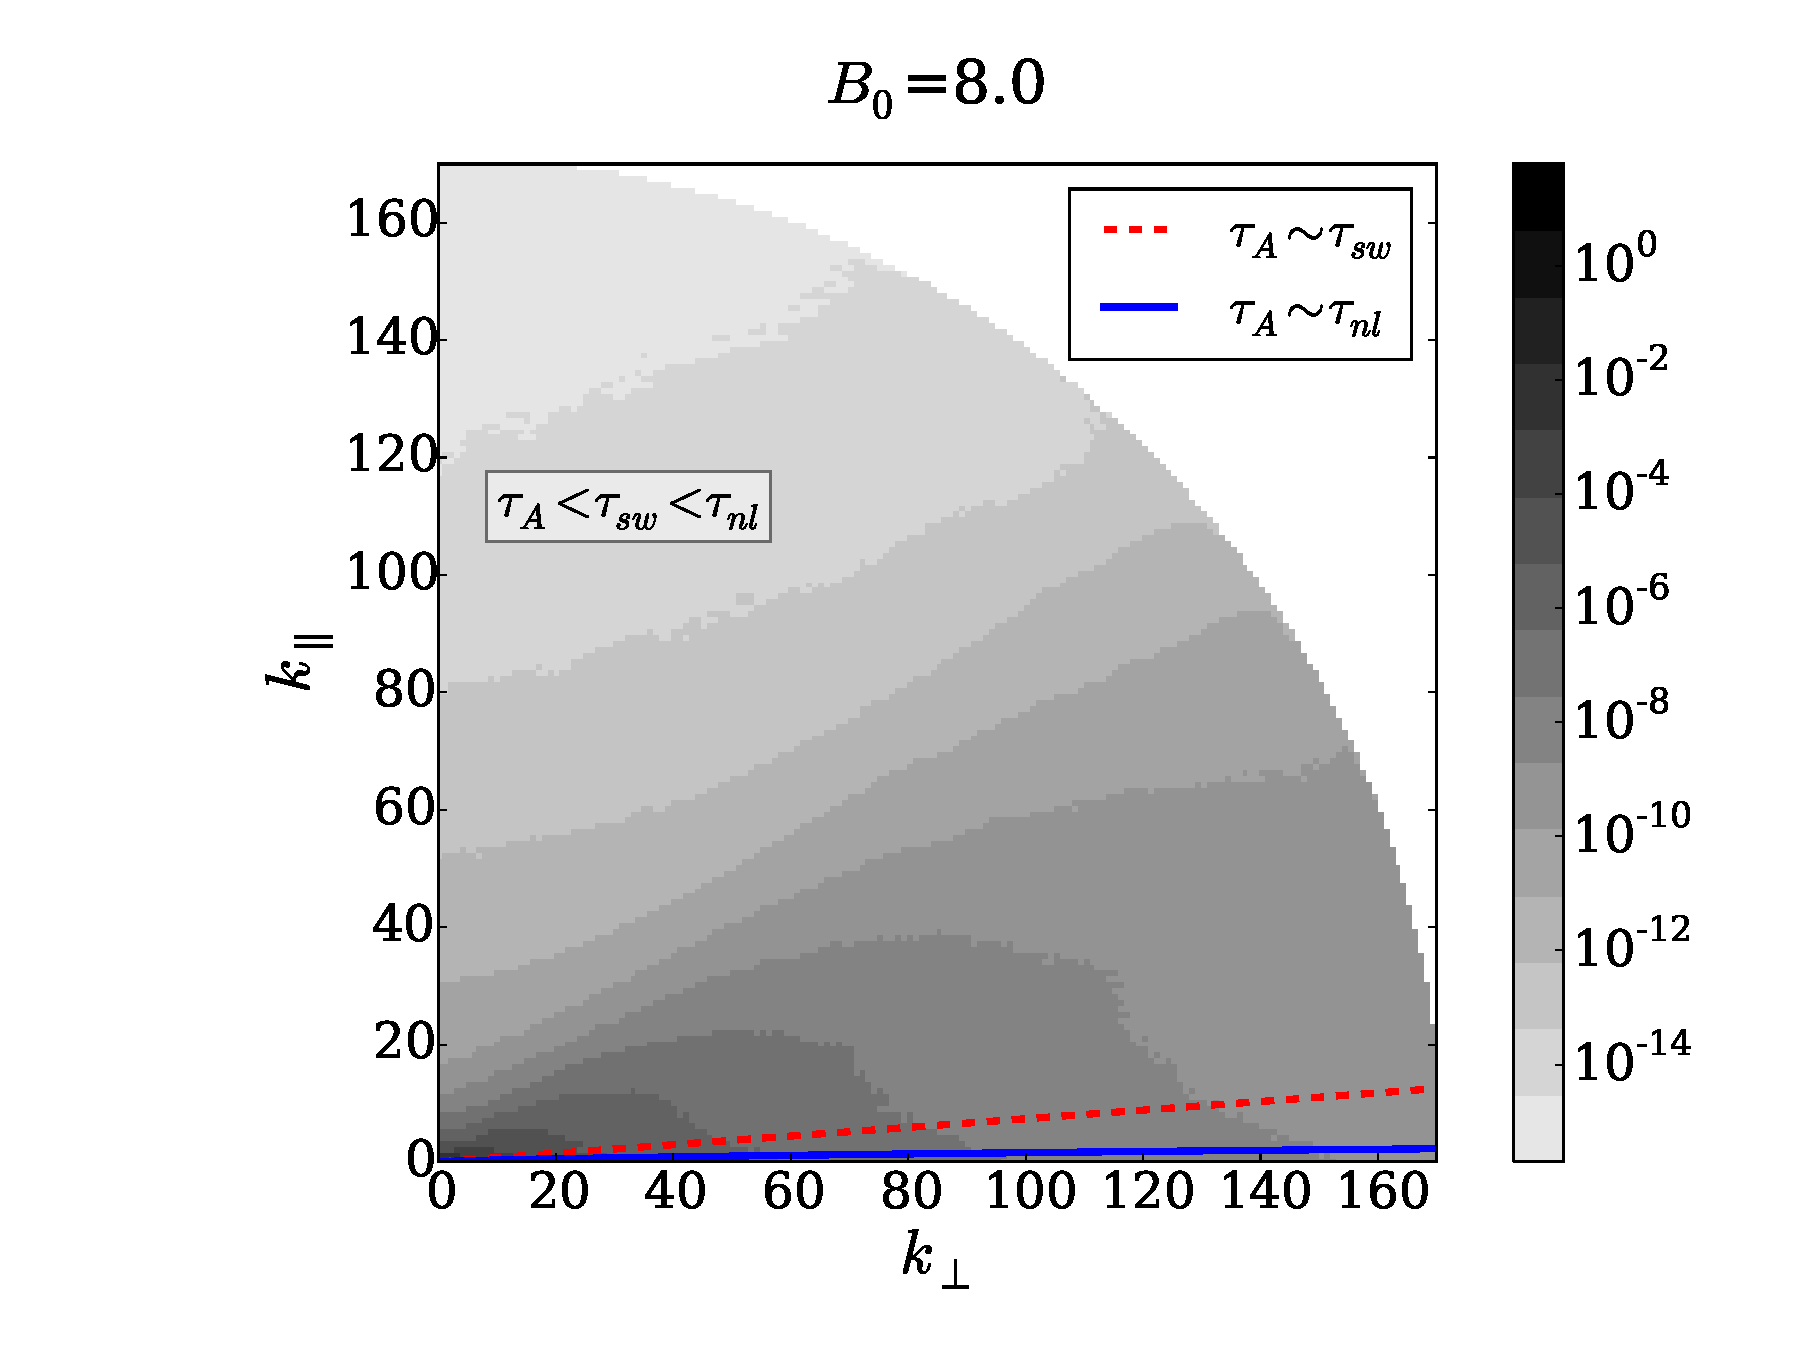
\includegraphics[width=0.48\textwidth]{SpatioTemporalSpectra/fig2_B8.pdf}}
  \subfigure[$B_0=8$ in log-log scale]{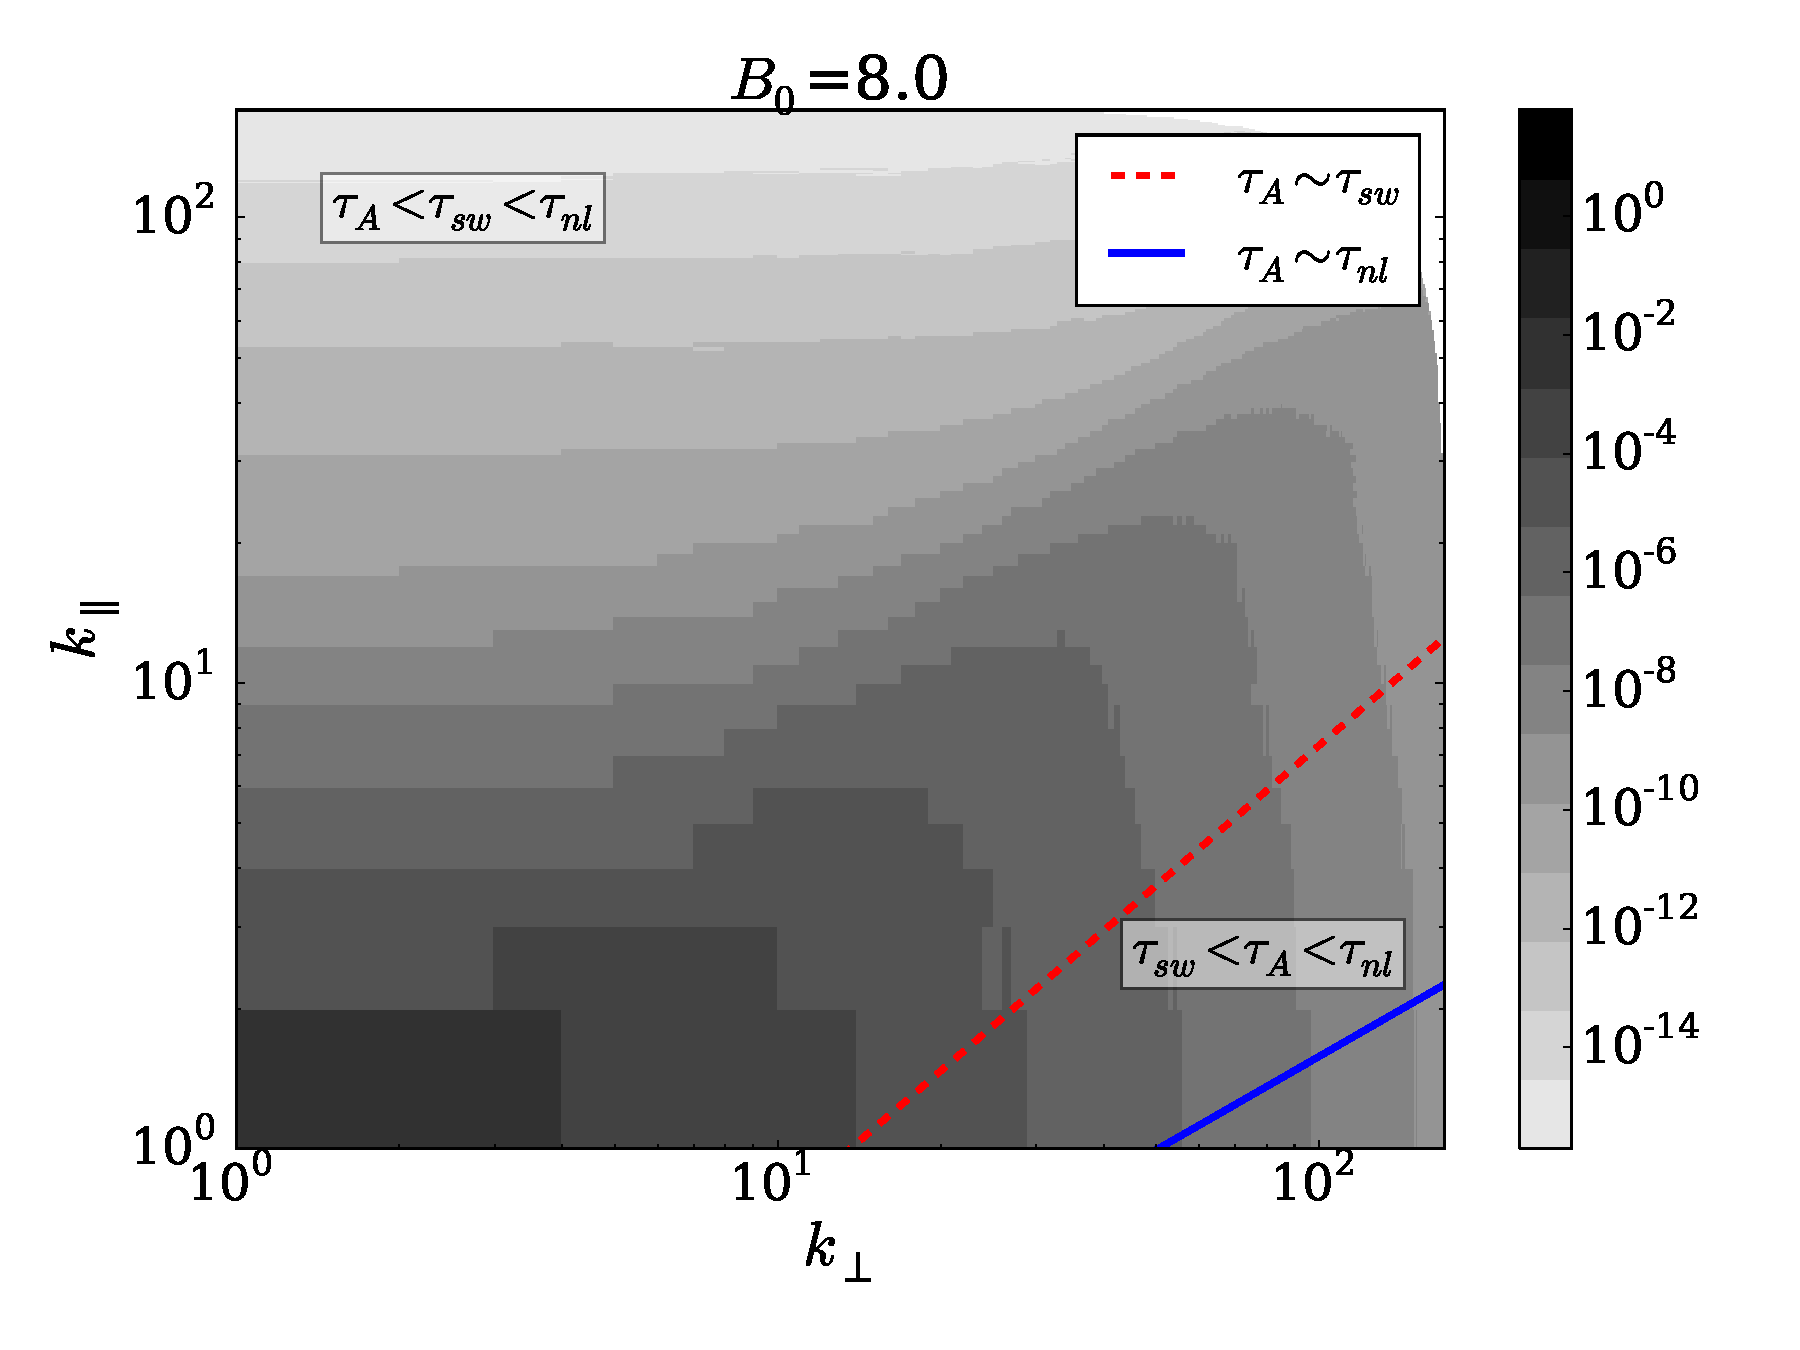
\includegraphics[width=0.48\textwidth]{SpatioTemporalSpectra/fig2_B8_log.pdf}}
%  \subfigure[$B_0=8$ in log-log scale]{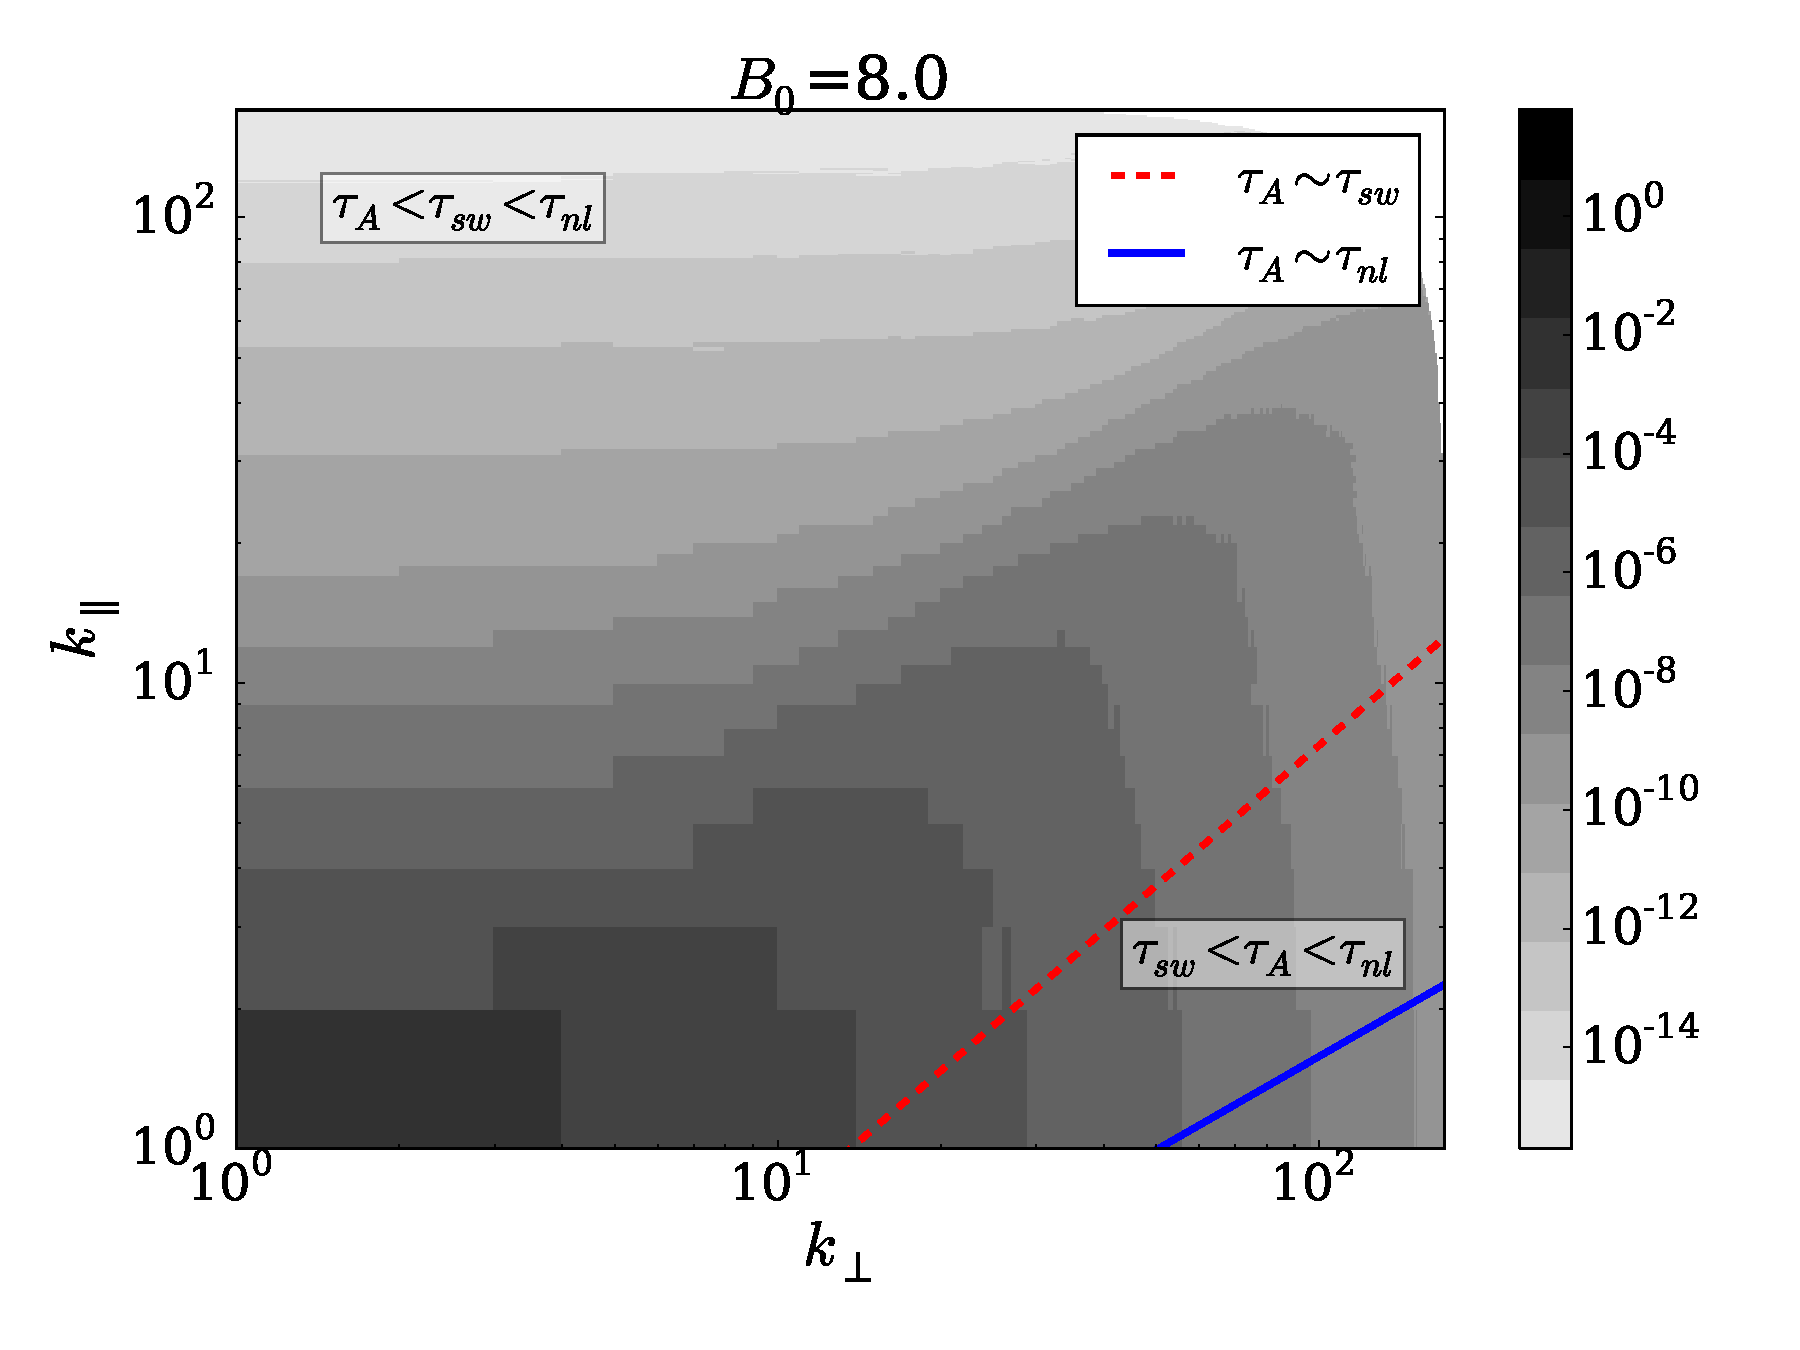
\includegraphics[width=0.45\textwidth]{SpatioTemporalSpectra/fig2_B8_log.eps}}
  \caption{Isocontours of the axisymmetric energy spectrum
    $e(k_\perp,k_\parallel)$ for $B_0=0$, $1$, $4$ and $8$. The cases
    with $B_0=4$ and $8$ are also ploted in a log-log scale to show
    with more detail the inertial range. In all cases, dark means
    larger energy density (in logarithmic scale). The lines indicate
    the modes for which sweeping time or local non-linear time become
    equal to the Alfv\'en time. For large $B_0$ the isocontours change
    shape as they cross each of these lines. Note also the stronger
    anisotropy of the spectrum as $B_0$ increases, as well as the
    increase in the surface covered by modes which have the Alfv\'en
    period as the fastest time.}
  \label{fig2:isocontourns}
\end{figure*}


\subsection{Spatio-temporal spectra}

La figura \cref{fig3:B025_bvf_Etot_kperp0} (para la simulación con
$B_0=0.25$), la \cref{fig3:B1_bvf_Etot_kperp0} ($B_0=1$) y la
\cref{fig3:B8_bvf_Etot_kperp0} ($B_0=8$) muestran el espectro en
función del vector de onda y la frecuencia, $E(\vec{k},
\omega)/E(\vec{k})$, para modos $\vec{k}$ con $k_\perp = 0$, donde
\begin{equation}
  E(\vec{k})=\int E(\vec{k},\omega)d\omega
\end{equation}
es el espectro de la energía total. Con esta elección para la
normalización, resultan más claramente visibles las frecuencias que
concentran la mayor cantidad de energía para cada $\vec{k}$. Para
$B_0=0.25$ (\cref{fig3:B025_bvf_Etot_kperp0}) observamos una clara
dispersión de la energía por debajo de la línea de la relación de
\sweeping (i.e., vemos excitaciones en todos los modos con frecuencias
iguales o menores que $\omega = v_{rms} k_\parallel$, indicando que
las estructuras de escalas pequeñas están siendo advectadas por todas
las velocidades iguales o menores a $v_{rms}$).  También es observable
para valores pequeños de $k_\parallel$ una acumulación débil cerca de
la relación de dispersión de Alfvén $\omega = B_0 k_\parallel$, aunque
el amplio espectro en el dominio de las frecuencias sugiere que el
\sweeping es dominante en este caso.

Al incremental el campo medio a $B_0=1$
(\cref{fig3:B1_bvf_Etot_kperp0}), parte de la energía se concentra por
encima de la línea se \sweeping, y comienza a seguir la relación de
dispersión de Alfvén, aunque el espectro continúa siendo muy amplio en
las frecuencias, con la mayor parte de la energía por debajo de la
relación de \sweeping.  Este comportamiento cambia drásticamente para
valores más altos de $B_0$.  En la \cref{fig3:B8_bvf_Etot_kperp0}
($B_0=8$), podemos ver que la energía claramente se concentra
alrededor de la relación de dispersión de las ondas de Alfvén, con un
pico de concentración para modos con hasta $k_\parallel \approx 10$,
para posteriormente dispersarse hacia la relación de \sweeping para
números de onda más grandes.  Notar que este comportamiento indica una
competición entre el tiempo magnetohidrodinámico de \sweeping y el
tiempo de Alvén, con este último resultando dominante a grandes
escalas para valores de $B_0$ grandes. Estos resultados respaldan y
mejoran los obtenidos por Dmitruk and Matthaeus
\cite{dmitruk_waves_2009}, y son compatibles para números de onda
pequeños y $B_0$ grande con los obtenidos recientemente en
\cite{meyrand_direct_2016, meyrand_weak_2015}. En particular, Meyrand
\cite{meyrand_direct_2016} también reporta una transición de un
espectro ondular estrecho a un espectro más amplio, aunque la escala y
el mecanismo responsable para esta transición no fue estudiado. Como
confirmaremos en la próxima sección a partir de las funciones de
descorrelación, la competición entre los tiempos de \sweeping y de
Alfvén como el tiempo de descorrelación dominante, es responsable del
cambio observado en el comportamiento del espectro.

\begin{figure}
  \centering 
  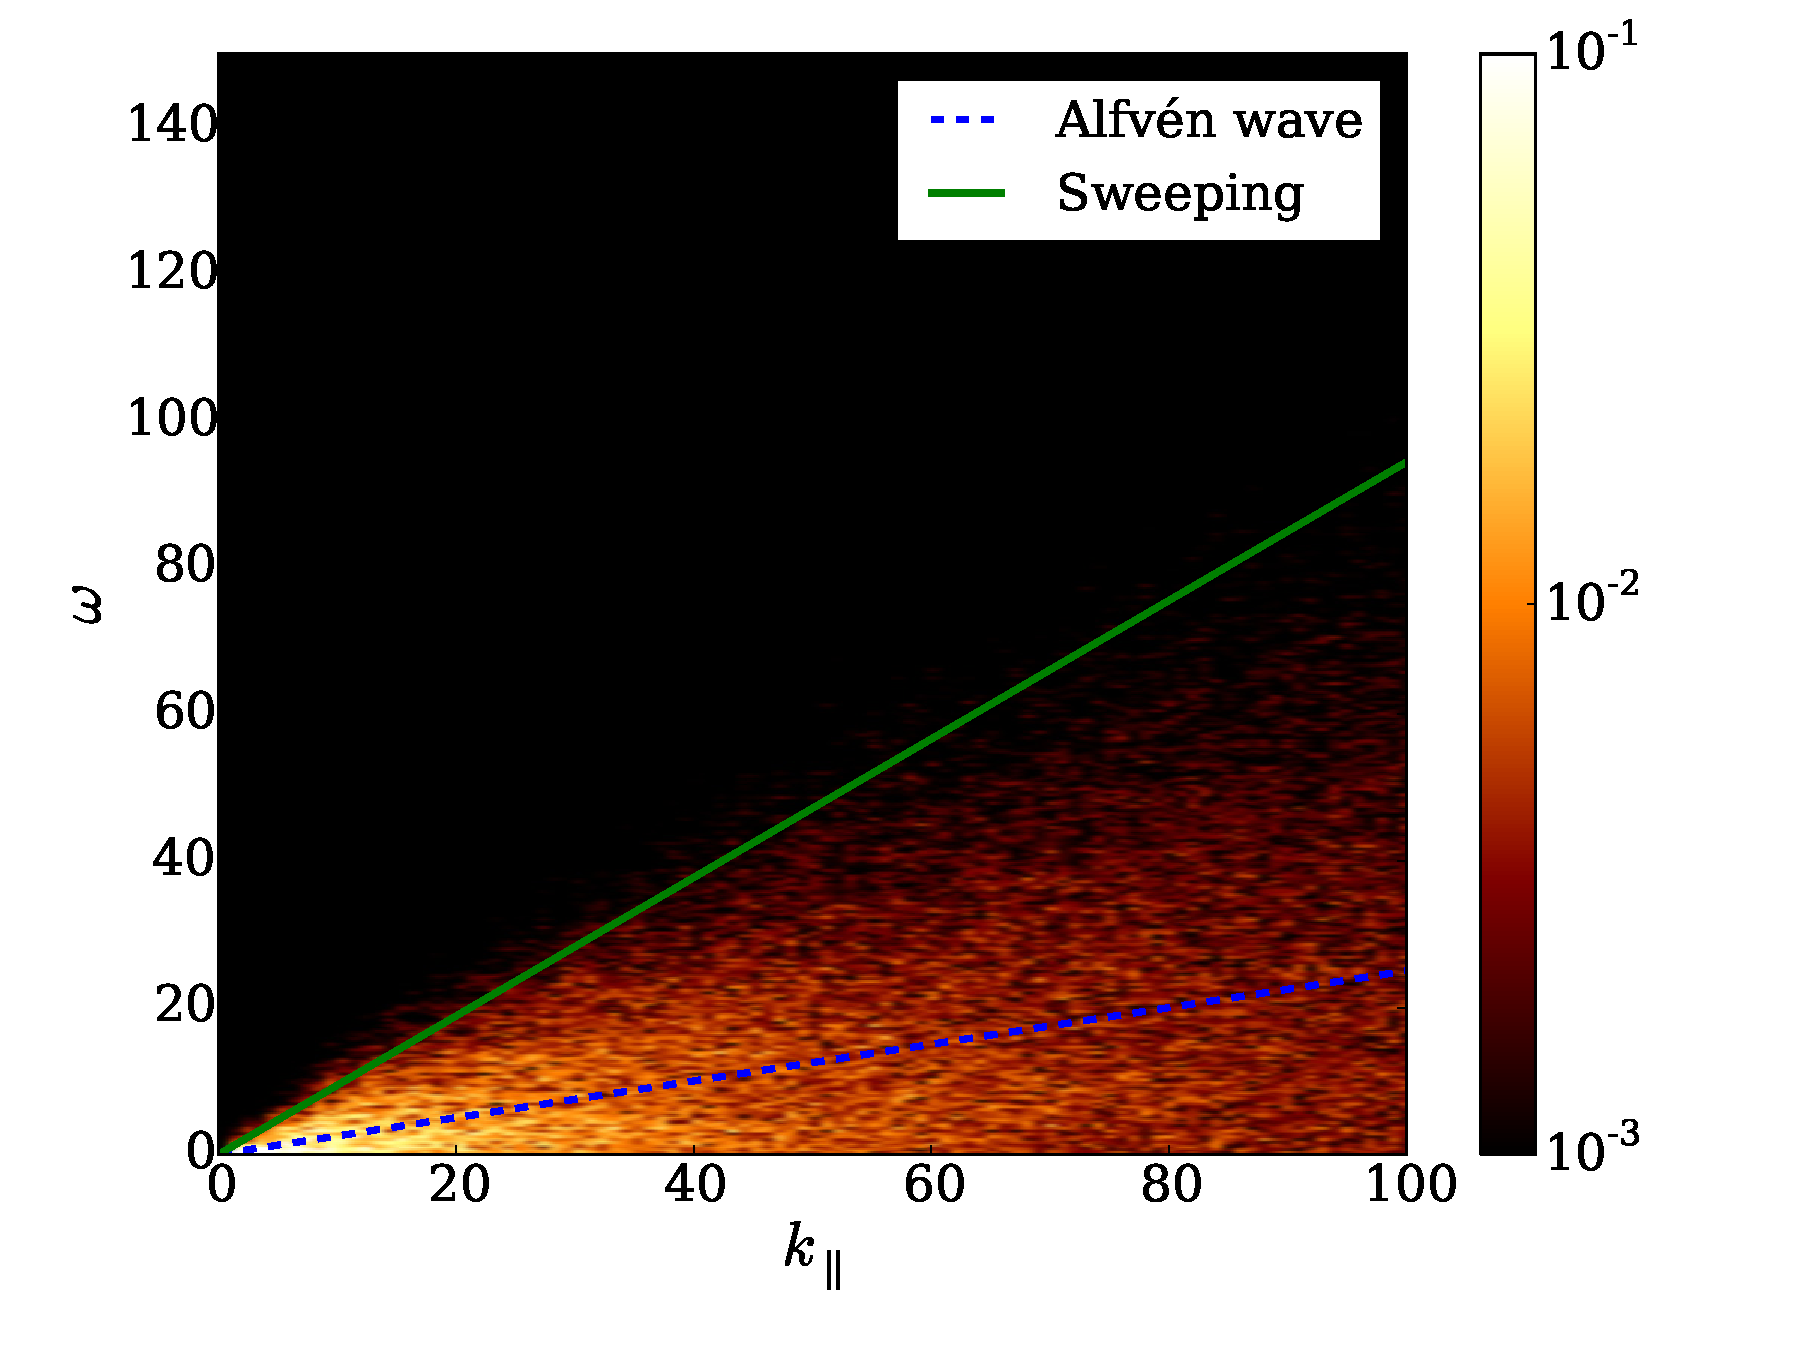
\includegraphics[width=1\columnwidth]{SpatioTemporalSpectra/fig3_B025_Etot-eps-converted-to.pdf}
  \caption{Normalized wave vector and frequency spectrum $E(\vec{k},
    \omega)/E(\vec{k})$ for the run with $\vec{B_0}=0.25$, for modes
    with $k_\perp=0$, and thus as a function of $k_\parallel$. Lighter
    regions indicate larger energy density. The spectrum corresponds
    to the power in the time and space Fourier transform of the
    fields, such that accumulation of energy in modes near the
    dispersion relation (or in all modes below the sweeping curve)
    indicates dominance of a physical effect (i.e., of its associated
    frequency) in the dynamics of a given scale $\sim
    1/k_\parallel$. The dashed (blue) line indicates the dispersion
    relation for Alfv\'en waves, and the continuous (green) line
    indicates the sweeping relation. A broad excitation of modes is
    observed for all modes with $\omega \leq v_{rms} k_\parallel$
    (sweeping), while only a very weak accumulation at small
    $k_\parallel$ can be seen for $\omega=B_0 k_\parallel$
    (Alfv\'en).}
  \label{fig3:B025_bvf_Etot_kperp0}
\end{figure}

\begin{figure}
  \centering
  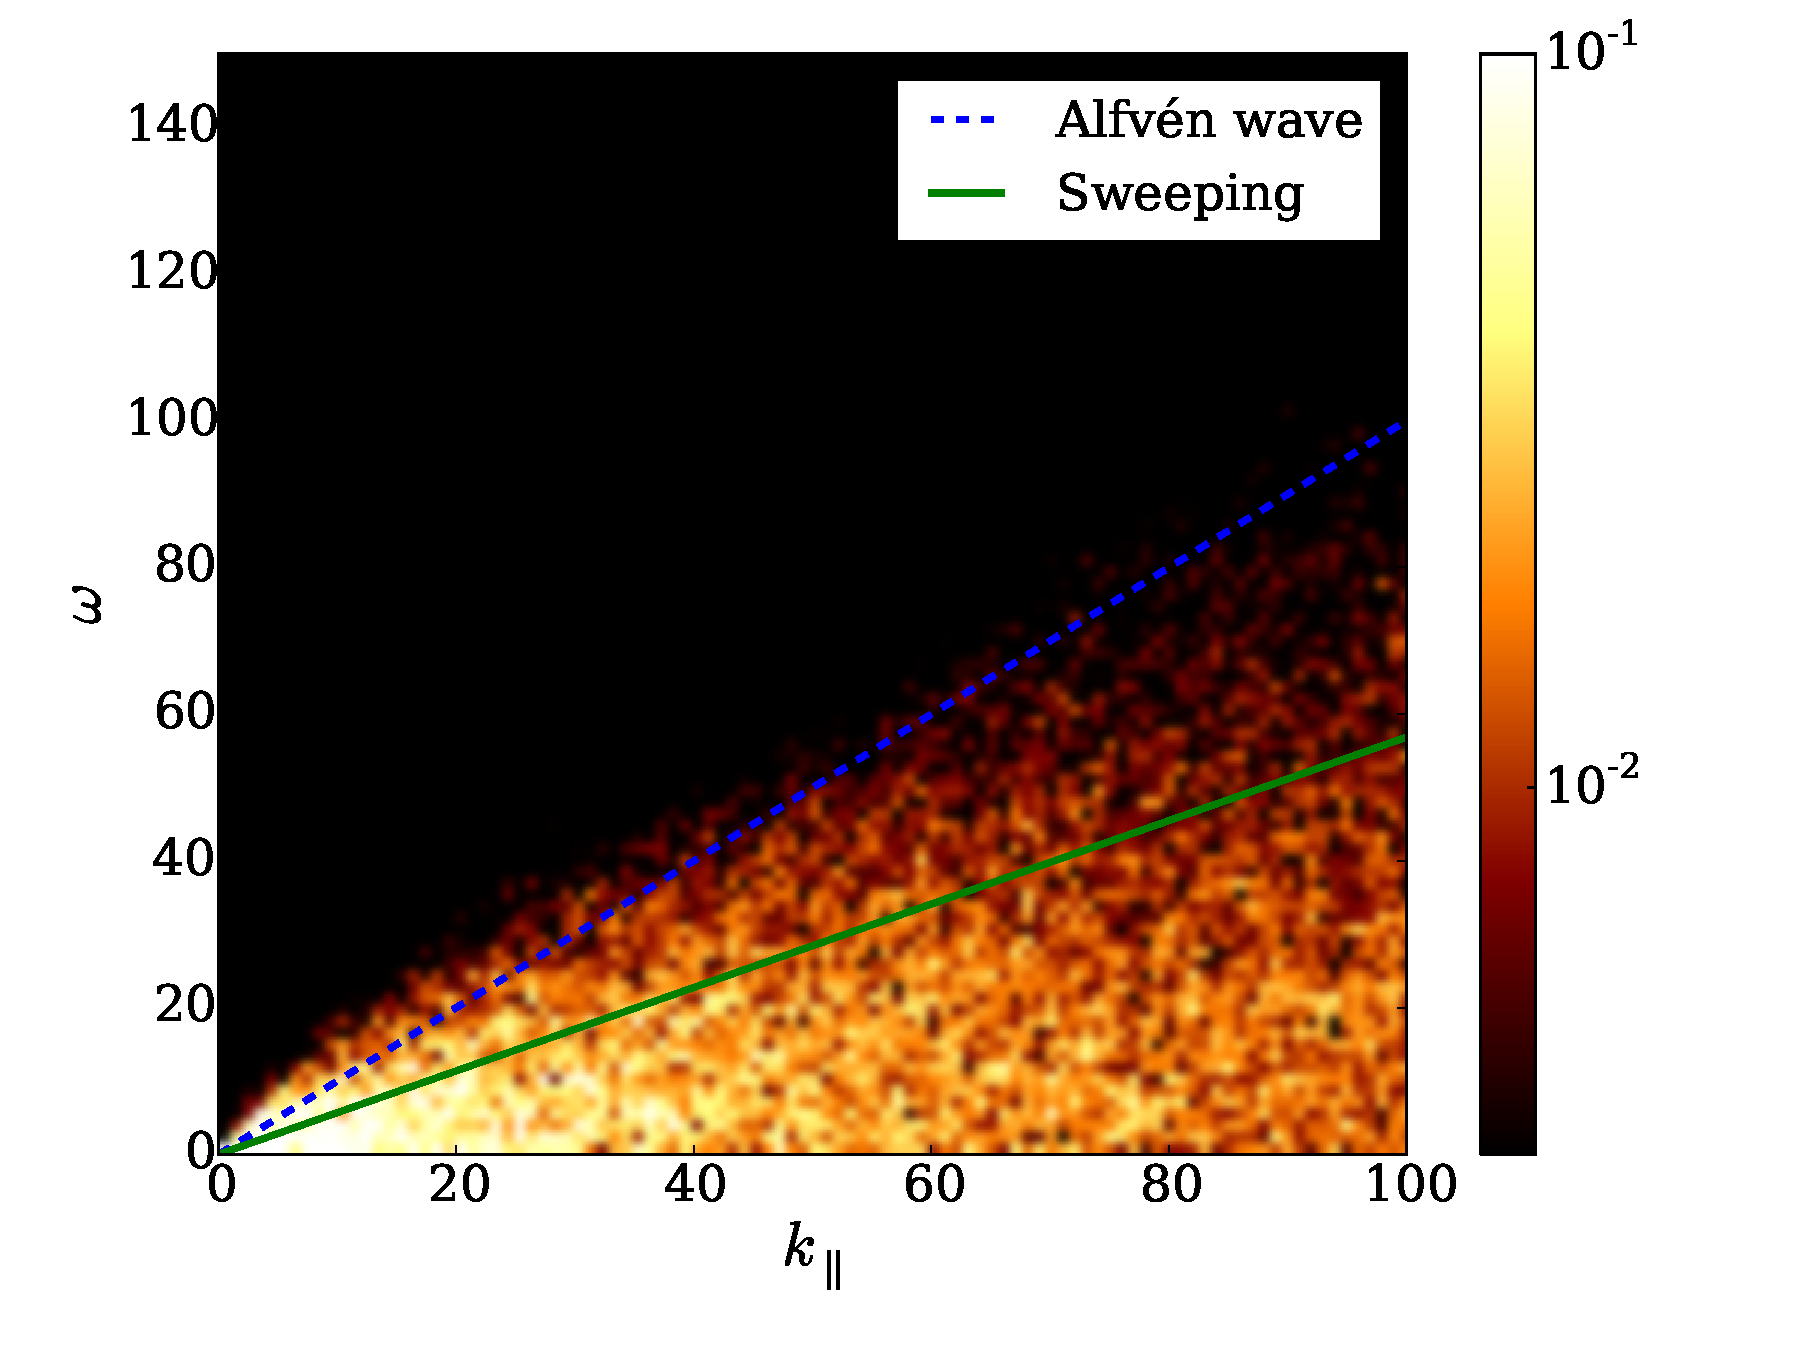
\includegraphics[width=1\columnwidth]{SpatioTemporalSpectra/fig3_B1_Etot-eps-converted-to.pdf}
  \caption{Normalized wave vector and frequency spectrum $E(\vec{k},
    \omega)/E(\vec{k})$ for the run with $B_0=1$, for modes with
    $k_\perp=0$, and thus as a function of $k_\parallel$ and
    $\omega$. Lighter regions indicate larger energy density. The
    dashed (blue) line indicates the dispersion relation for Alfv\'en
    waves and the continuous (green) line indicates the sweeping
    relation.}
  \label{fig3:B1_bvf_Etot_kperp0}
\end{figure}

\begin{figure}
  \centering
  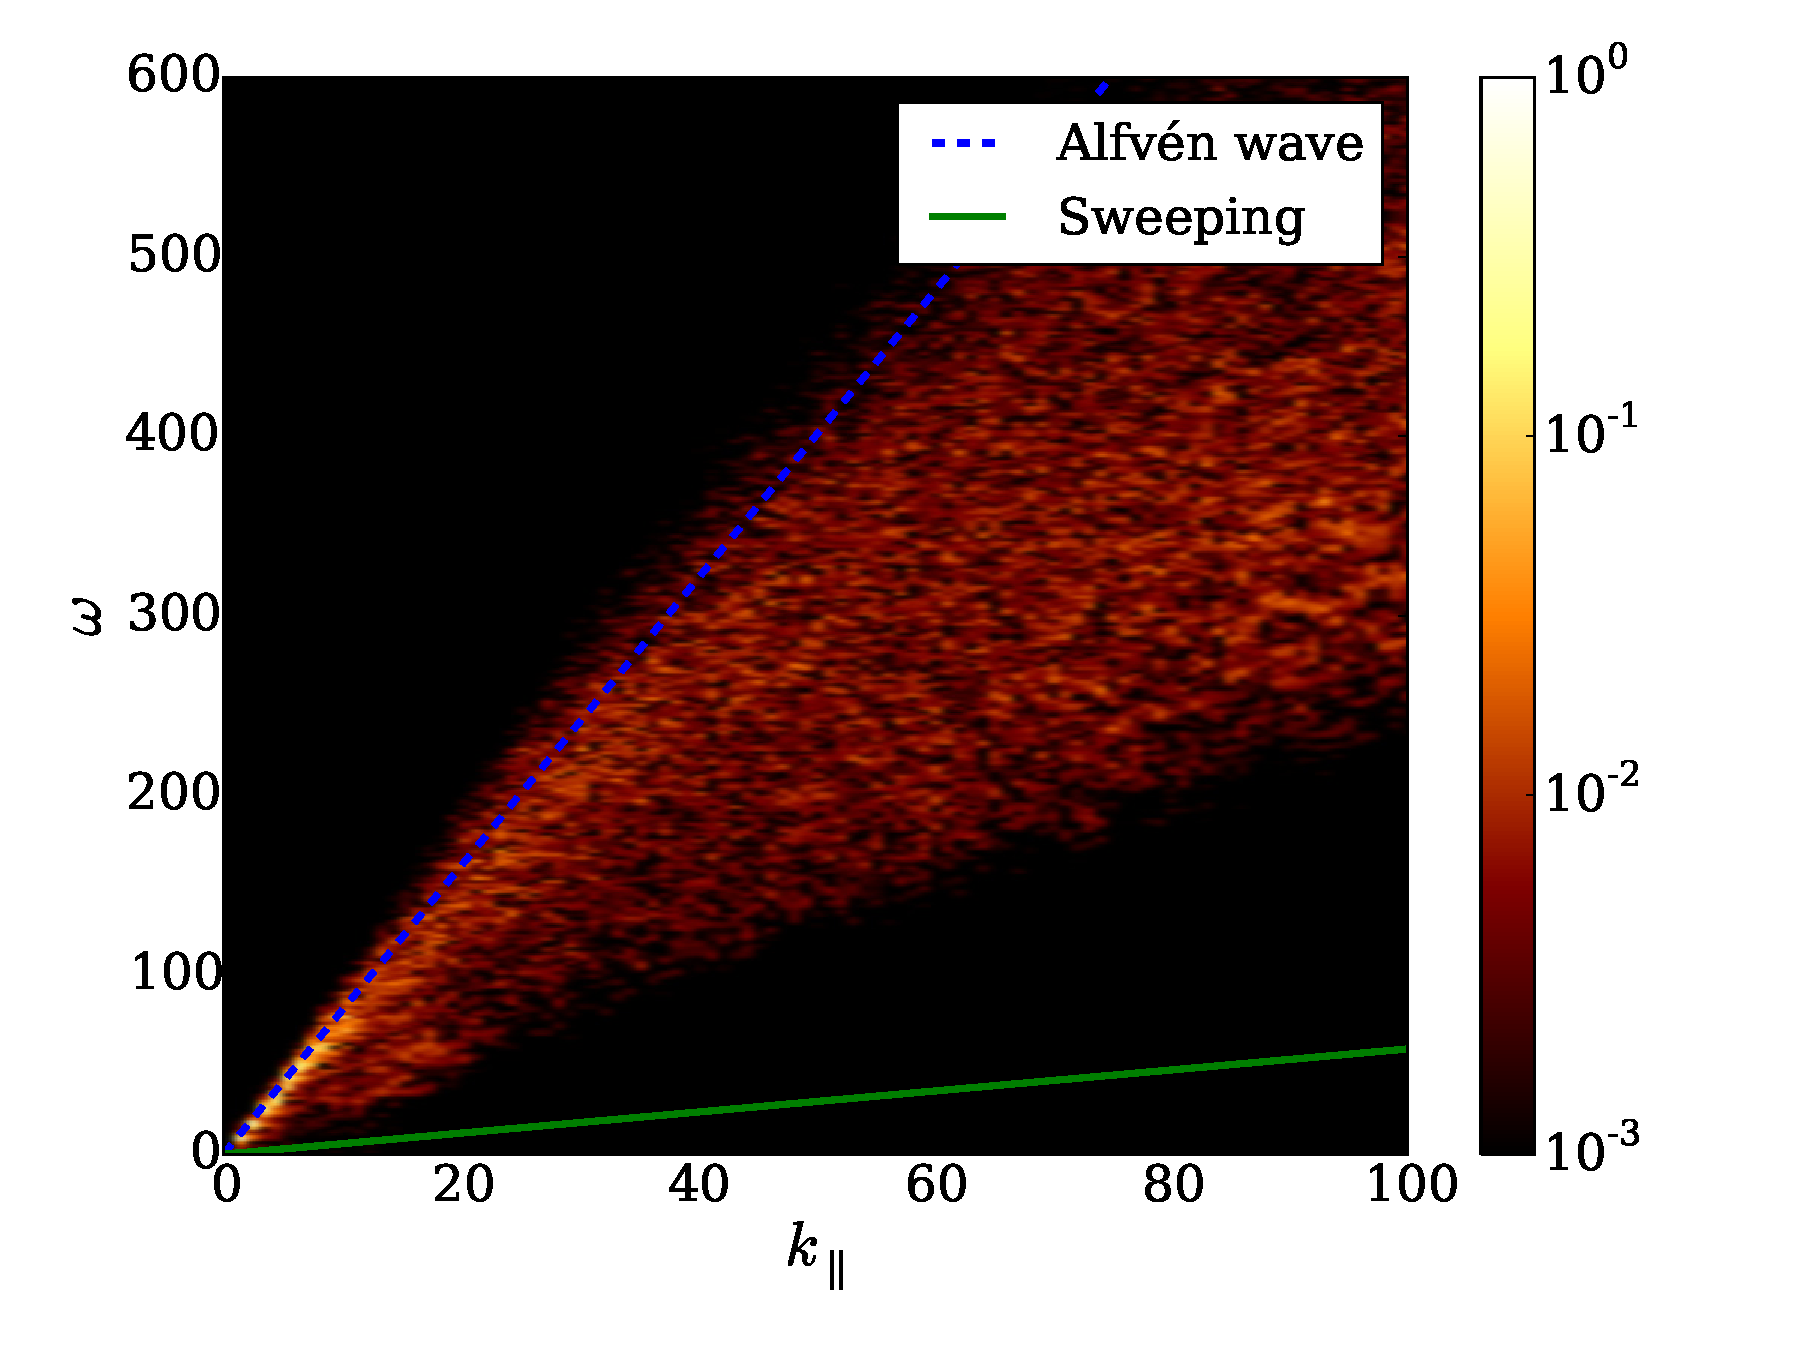
\includegraphics[width=1\columnwidth]{SpatioTemporalSpectra/fig3_B8_Etot-eps-converted-to.pdf}
  \caption{Normalized wave vector and frequency spectrum $E(\vec{k},
    \omega)/E(\vec{k})$ for the run with $B_0=8$, for modes with
    $k_\perp=0$, and thus as a function of $k_\parallel$ and
    $\omega$. Lighter regions indicate larger energy density. The
    dashed (blue) line indicates the dispersion relation for Alfv\'en
    waves and the continuous (green) line indicates the sweeping
    relation. Note in this case power is concentrated in a narrow
    region near the wave dispersion relation up to 
    $k_\parallel \approx 10$, corresponding to Alfv\'enic
    excitations.}
  \label{fig3:B8_bvf_Etot_kperp0}
\end{figure}


\begin{figure}
  \centering
  \subfigure[$\Gamma(k_\perp=0,k_\parallel=k_0,\tau)$]{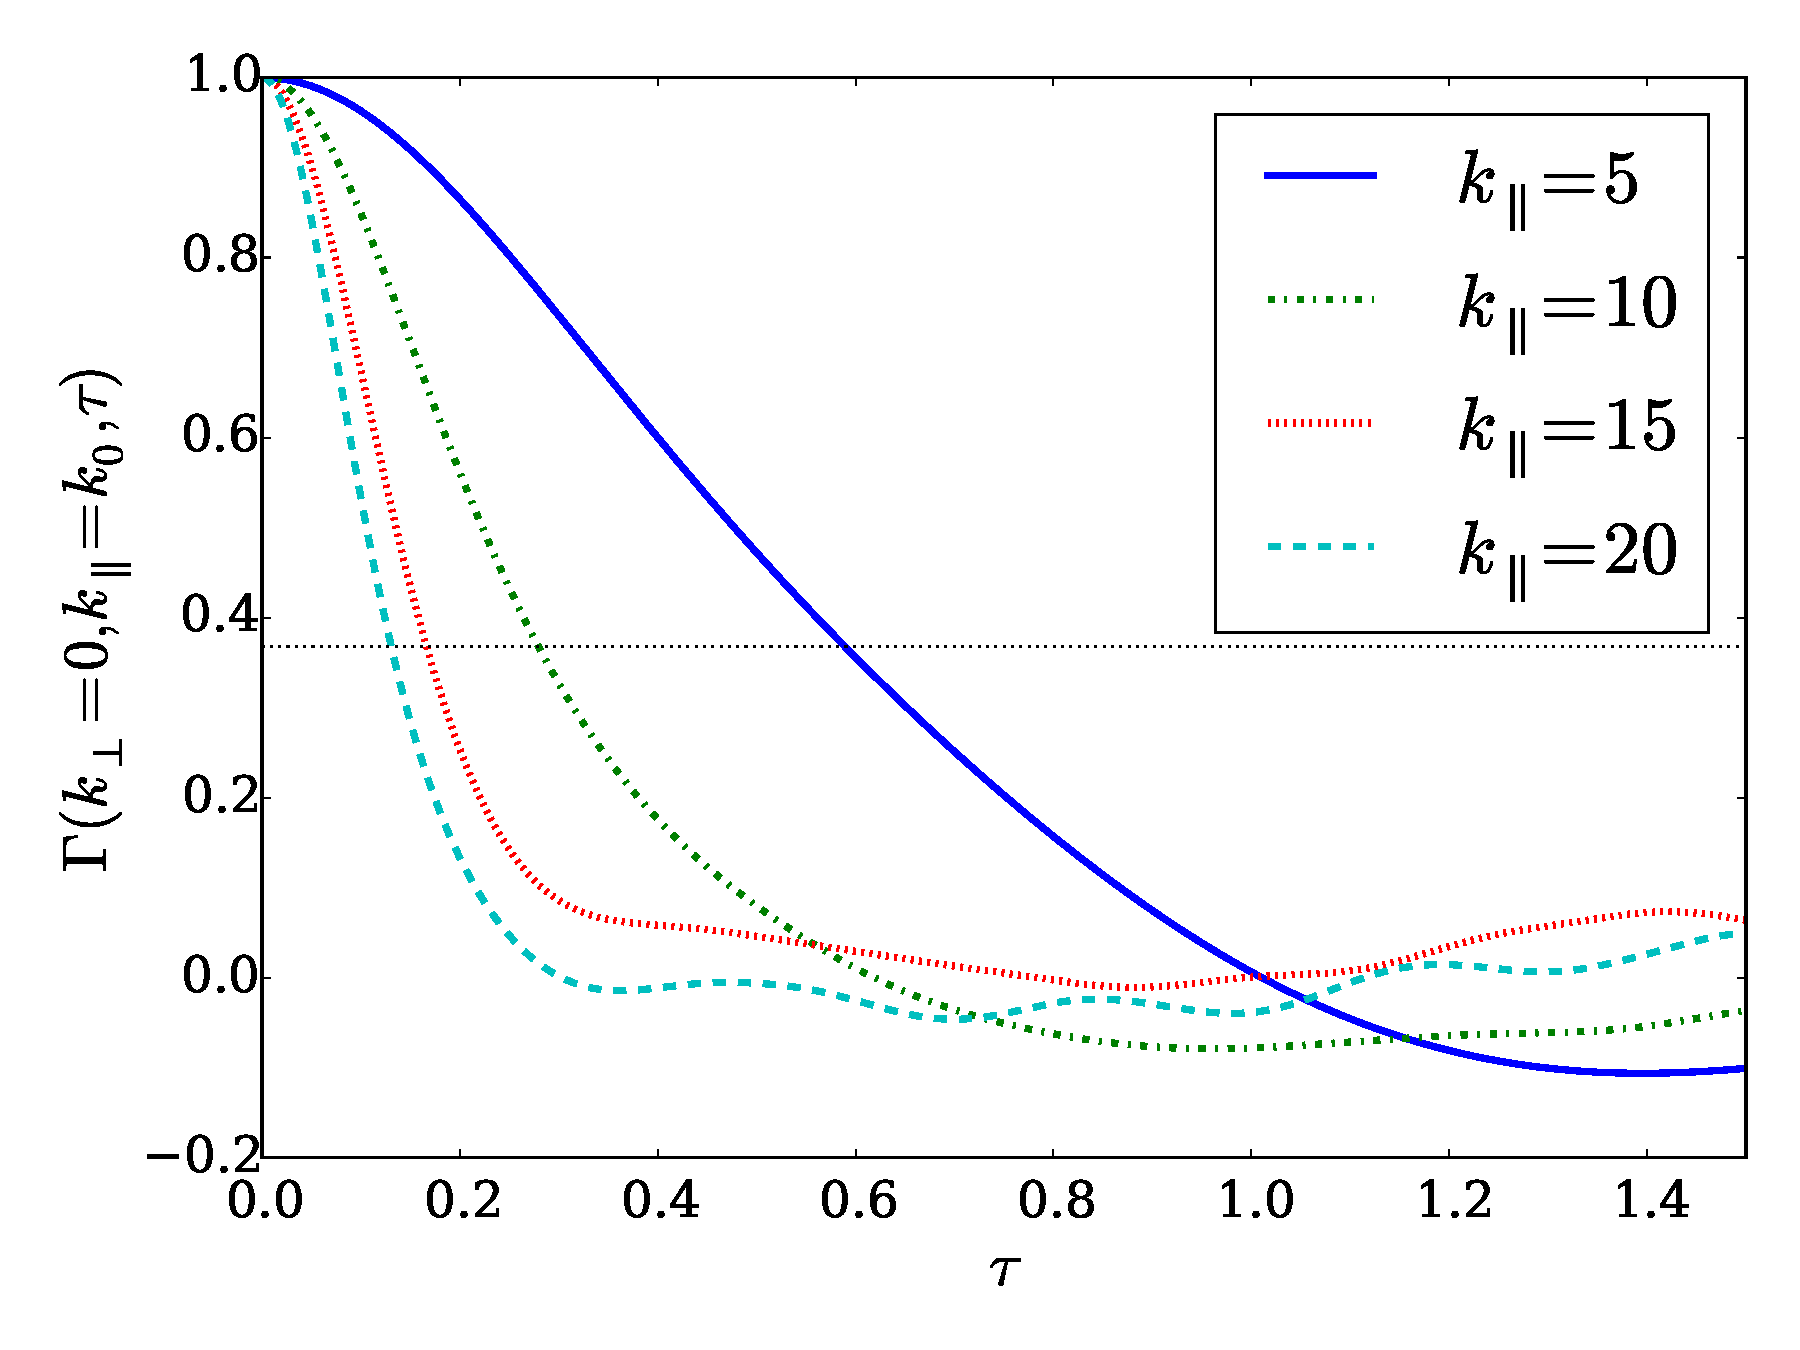
\includegraphics[width=1\columnwidth]{SpatioTemporalSpectra/fig4_B1_b_kperp-eps-converted-to.pdf}}

  \subfigure[$\Gamma(k_\perp=k_0,k_\parallel=0,\tau)$]{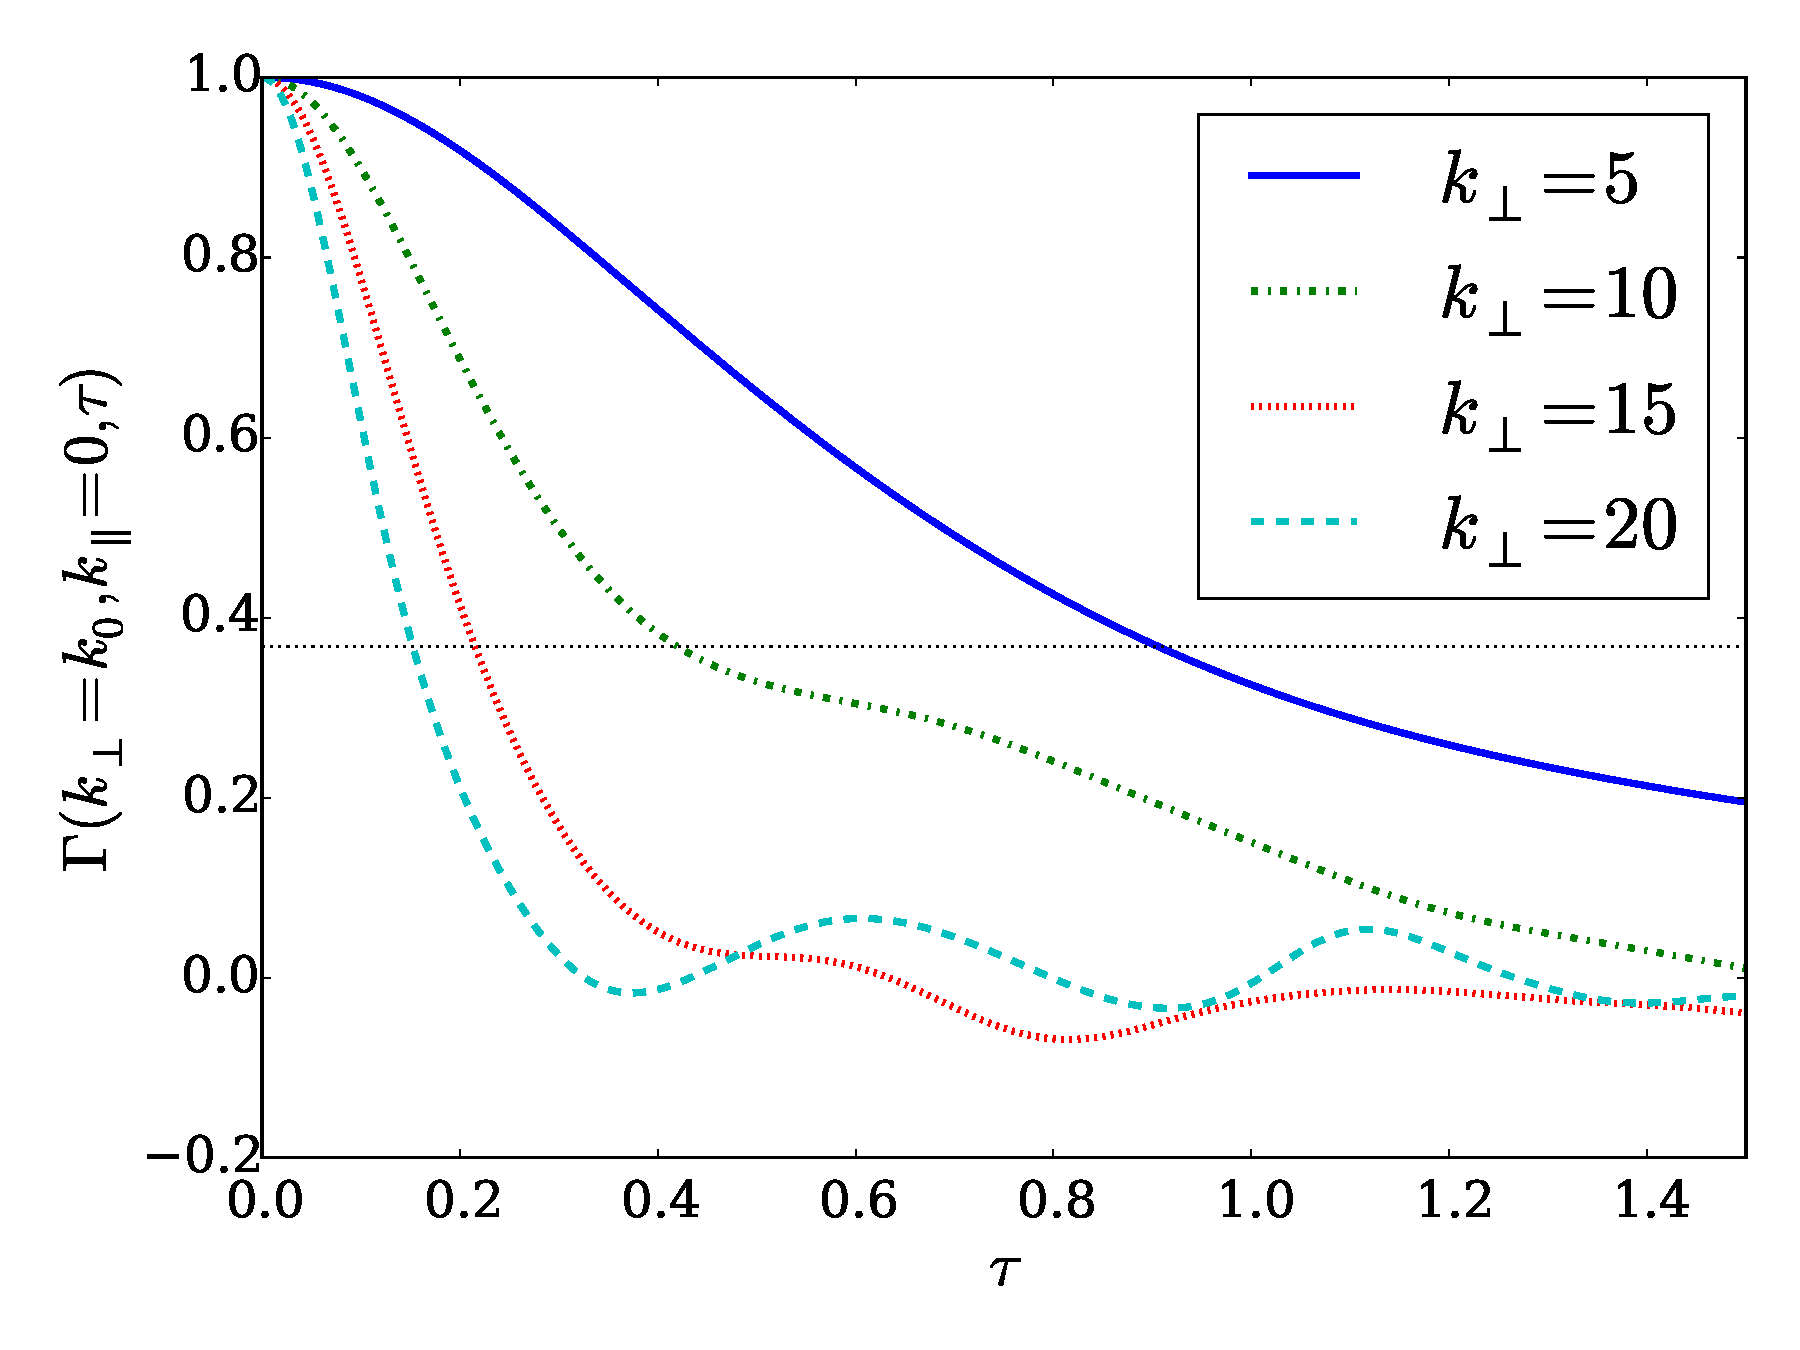
\includegraphics[width=1\columnwidth]{SpatioTemporalSpectra/fig4_B1_b_kpara-eps-converted-to.pdf}}
  \caption{Correlation functions
    $\Gamma(k_\perp=0,k_\parallel=k_0,\tau)$ and
    $\Gamma(k_\perp=k_0,k_\parallel=0,\tau)$ as a function of the lag
    time $\tau$, for $k_0=5$, 10, 15, and 20, in the simulation with
    $B_0=1$. The value of $\tau$ for which $\Gamma=1/e$ (horizontal
    dotted line) corresponds to the decorrelation time $\tau_D$ for
    each value of $\vec{k}$.}
  \label{fig4:B1_bvf_b_kperp/kpara0}
\end{figure}


\subsection{Funciones de correlación y tiempos de descorrelación}

Con el fin de discernir entre los diferentes fenómenos (y escalas de
tiempo relevantes) que actúan en la turbulencia magnetohidrodinámica,
estudiamos las funciones de correlación $\Gamma(\vec{k},\tau)$, como
se explicó en detalle previamente en la sección
\ref{sec_Wfspectrum_and_Gamma}. Dado que nos enfocamos en la
turbulencia con un campo magnético guía, utilizamos $\Gamma(k_\perp,
k_\parallel, \tau)$ y consideramos varios valores de $(k_\perp,
k_\parallel)$ para estudiar la descorrelación como función del tiempo
de retraso $\tau$ a diferentes escalas.  En la
\cref{fig4:B1_bvf_b_kperp/kpara0}, se muestran las funciones de
correlación $\Gamma(k_\perp=0,k_\parallel=k_0,\tau)$ y
$\Gamma(k_\perp=k_0,k_\parallel=0,\tau)$ para diferentes valores de
$k_0$ para el caso del campo magnético externo moderado $B_0=1$. Aquí
podemos ver el comportamiento típico de las funciones de correlación,
con las escalas más grandes ($k$ más pequeños) tomándose un mayor
tiempo para descorrelacionarse. Se encontraron resultados similares
para los otros campos magnéticos externos considerados, $B_0=0$,
$0.25$, $4$, y $8$.

Para entender cuál de los diferentes tiempos (tiempo no lineal,
\sweeping aleatorio, y propagación de Alfvén) está controlando la
descorrelación temporal, necesitamos comparar la escala del tiempo de
descorrelación con la dependencia de escala teórica esperada para cada
proceso físico. Para hacer esto, usamos el hecho de que el modo con el
vector de onda $\vec{k}$ debe estar descorrelacionada después de un
tiempo $\tau_D(\vec{k})$, siguiendo aproximadamente un decaimiento
exponencial
\begin{equation}
\Gamma(\vec{k},\tau) \sim e^{-\tau/\tau_D(\vec{k})}.
\end{equation}
Por simplicidad, evaluamos $\tau_D(\vec{k})$ como el tiempo al cual la
función $\Gamma$ decaía a $1/e$ de su valor inicial..

\begin{figure}
  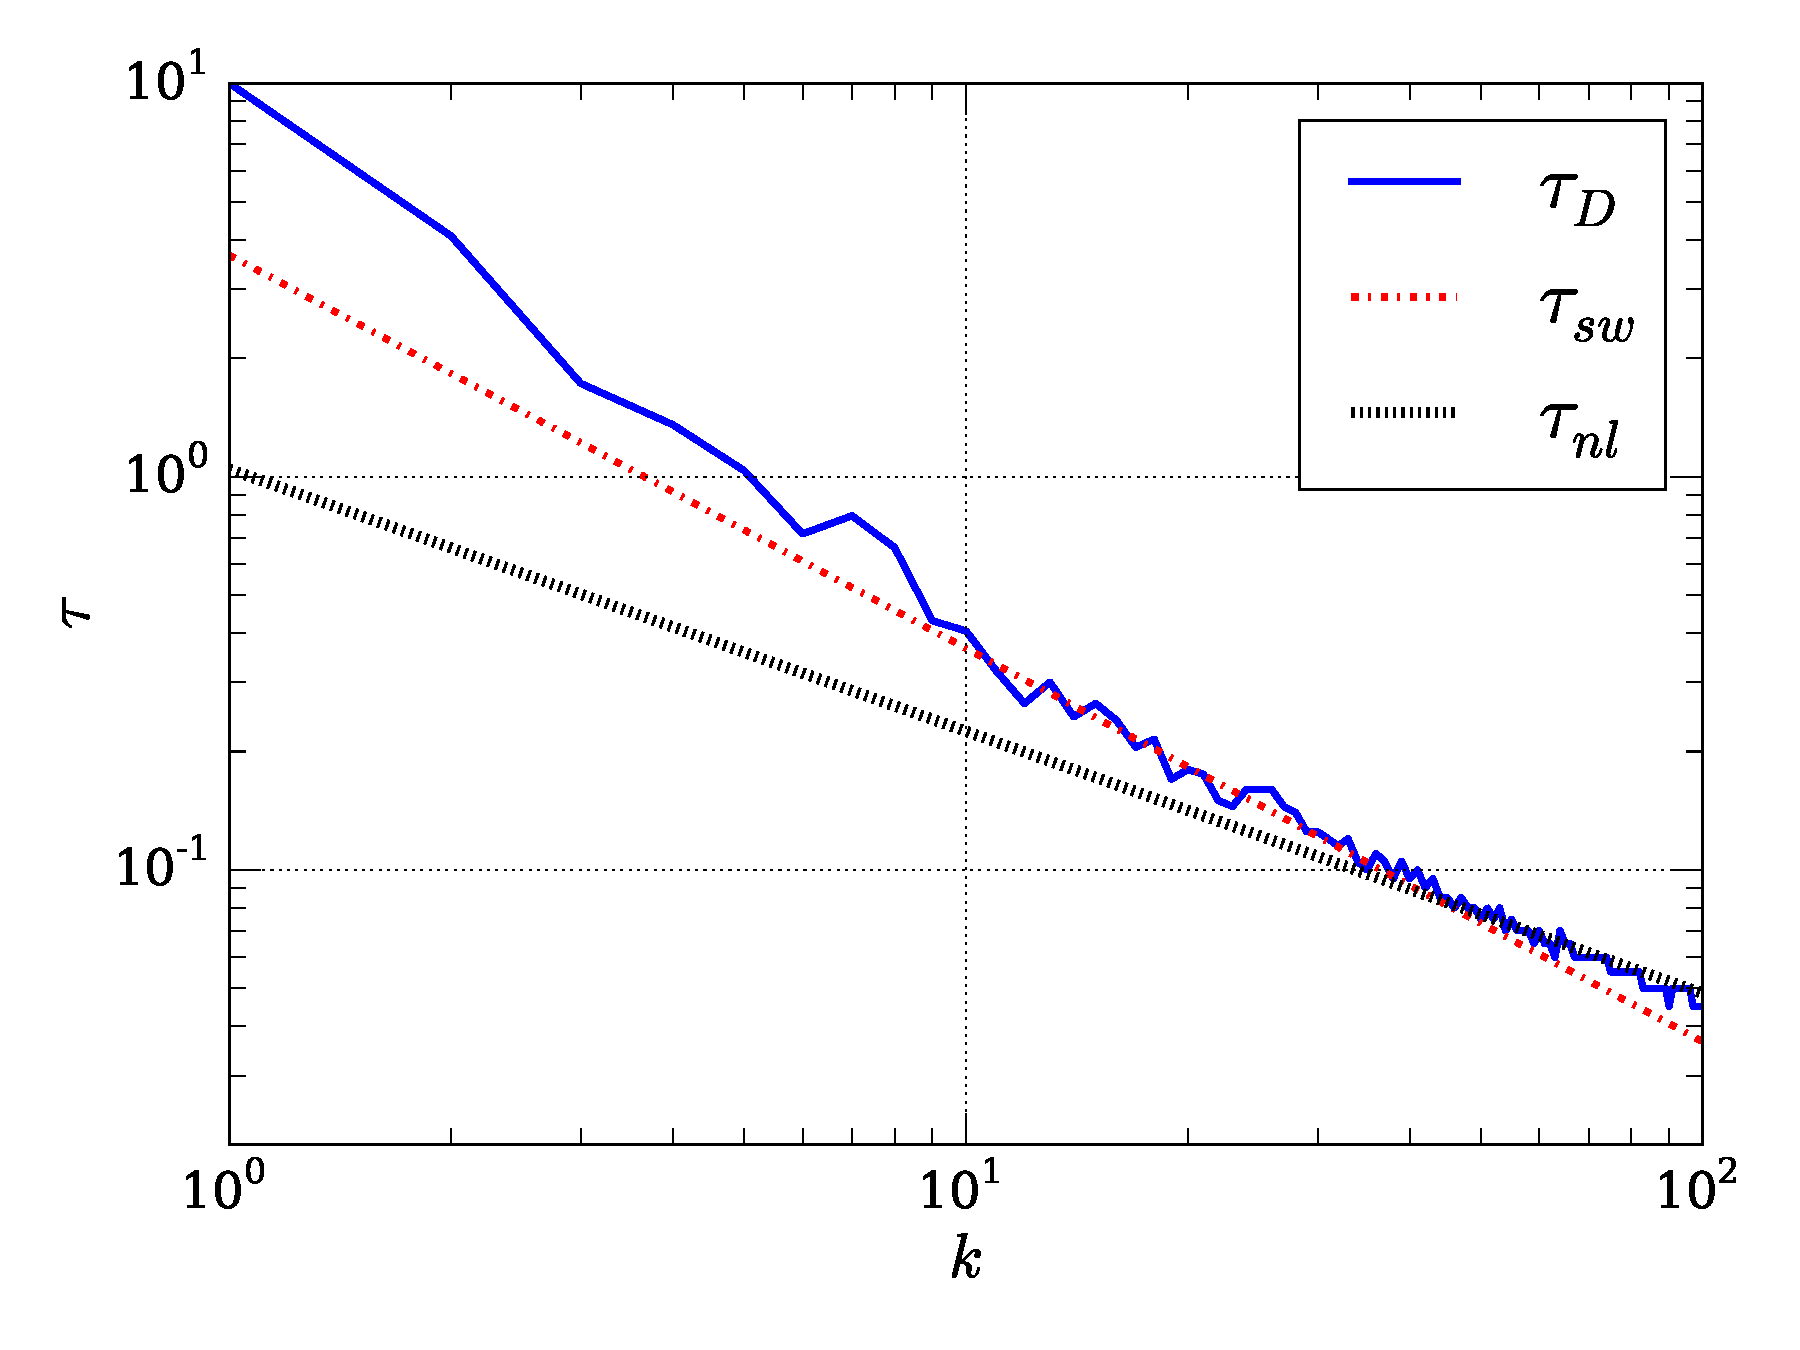
\includegraphics[width=1\columnwidth]{SpatioTemporalSpectra/fig5_B0_b-eps-converted-to.pdf}
  \caption{Decorrelation times as a function of $k=|\vec{k}|$ for the
    isotropic case $B_0=0$. The straight lines indicate the
    theoretical predictions corresponding to the sweeping time and the
    nonlinear time. Except at the largest wavenumbers, the
    decorrelation time seems to be dominated by sweeping.}
  \label{fig5:B0_bvf_b_kpara_0}
\end{figure}

Como primer ejemplo, la \cref{fig5:B0_bvf_b_kpara_0} muestra el tiempo
de descorrelación $\tau_D$ obtenido de $\Gamma(k,\tau)$ en el caso
isotrópico con $B_0=0$.  Podemos ver que la escala del tiempo de
descorrelación se encuentra en buen acuerdo con el tiempo de
\sweeping, excepto quizás para los números de onda más grandes (menor
escala).  Estos resultados son consistentes con los obtenidos por
Servidio {\it et al} \cite{servidio_time_2011} en el caso isotrópico.

Como se mencionó anteriormente, en el caso general puede ser difícil
diferenciar entre los efectos de \sweeping y de la propagación de
Alfvén, pues ambas escalas temporales varían como $k^{-1}$. Sin
embargo, en el caso anisotrópico (i.e., en presencia de un campo
guía), podemos hacer uso del escaleo observado respecto de los números
de onda paralelos y perpendiculares, para así hacer posible la
distinción.  En la \cref{fig5:B025_bvf_b_kperp} utilizamos resultados
de la simulación con $B_0=0.25$ para computar los tiempos de
descorrelación para los modos de Fourier en función de $k_\parallel$,
para varios valores fijos de $k_\perp$. Incluso para este caso con un
valor de $B_0$ relativamente pequeño, puede observarse que los tiempos
de descorrelación se encuentran más cerca del valor teórico esperado
del tiempo de \sweeping que de todos los otros tiempos (tiempo local
no lineal y tiempo Alfvénico). Esto es consistente con el resultado
obtenido a partir del espectro energético respecto del número de onda
y la frecuencia, mostrado previamente en la
\cref{fig3:B025_bvf_Etot_kperp0}. En la \cref{fig5:B025_bvf_b_kpara}
se puede ver una vista complementaria para la misma corrida con
$B_0=0.25$, donde se muestra el tiempo de descorrelación $\tau$ en
función de $k_\perp$ para varios valores fijados de $k_\parallel$. La
conclusión es nuevamente que el tiempo de \sweeping controla $\tau_D$
a todas las escalas, salvo las más grandes, ya que sólo para
$k_\perp=0$ y para $k_\parallel$ entre $\approx 1$ y $\approx 4$
$\tau_D$ se encuentra más cercano al tiempo de Alfvén.

La tendencia de que el tiempo de descorrelación sea controlado por el
\sweeping se puede ver nuevamente en la corrida con el campo medio
moderado $B_0=1$.  Estos resultados para el tiempo de descorrelación
se muestran en las \cref{fig5:B1_bvf_b_kperp,
  fig:B1_bvf_b_kpara}. Nuevamente, sólo para valores pequeños de
$k_{\parallel}$ y de $k_{\perp}=0$ el tiempo de descorrelación se
encuentra más cerca del tiempo de Alfvén. Esta tendencia pudo
observarse también en el espectro de la
\cref{fig3:B1_bvf_Etot_kperp0}.

\begin{figure}
  \centering
  \subfigure[$k_\perp=0$]{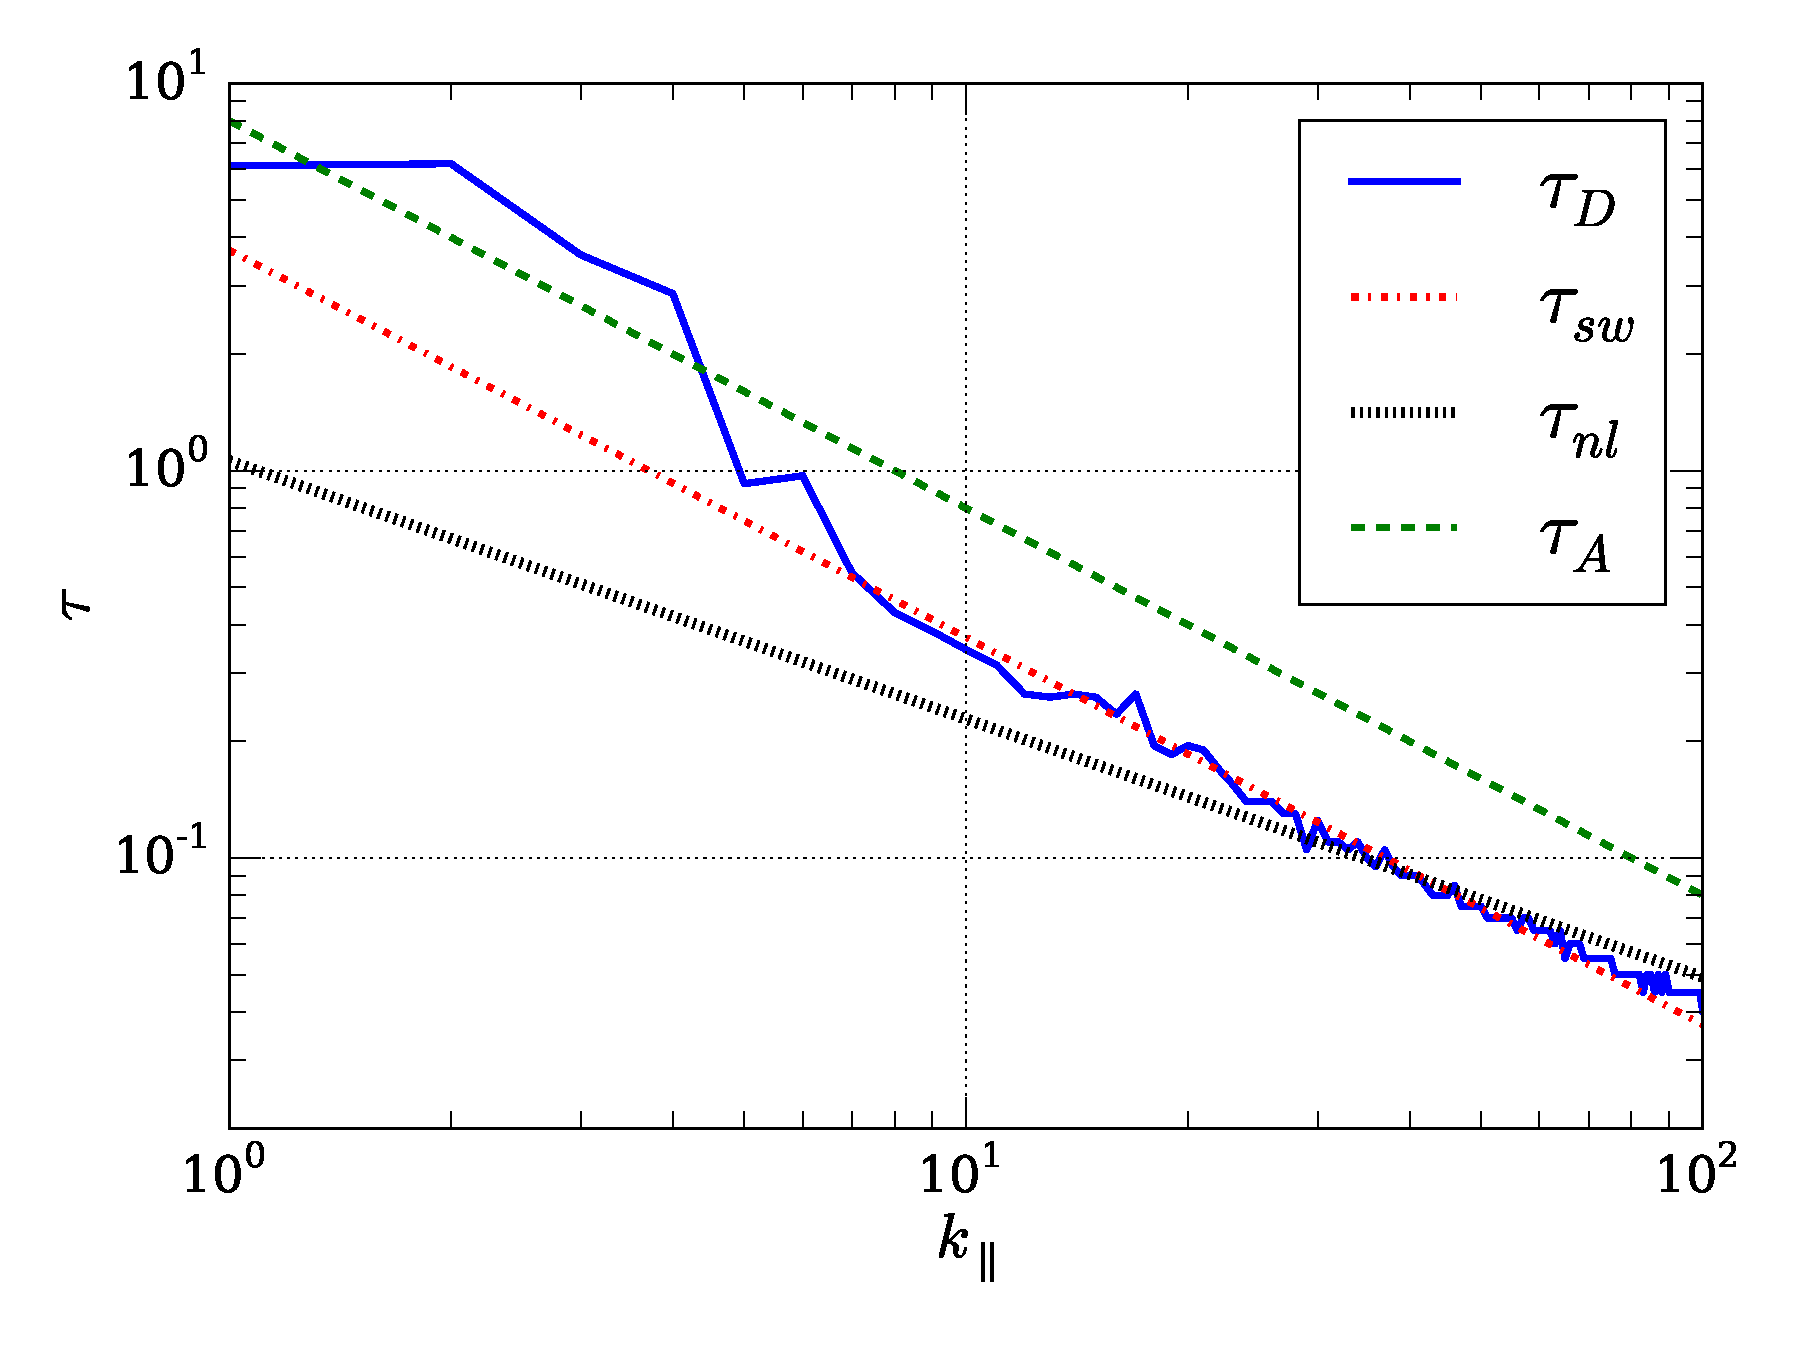
\includegraphics[width=1\columnwidth]{SpatioTemporalSpectra/fig5_B025_b_kperp_0-eps-converted-to.pdf}}

  \subfigure[$k_\perp=10$]{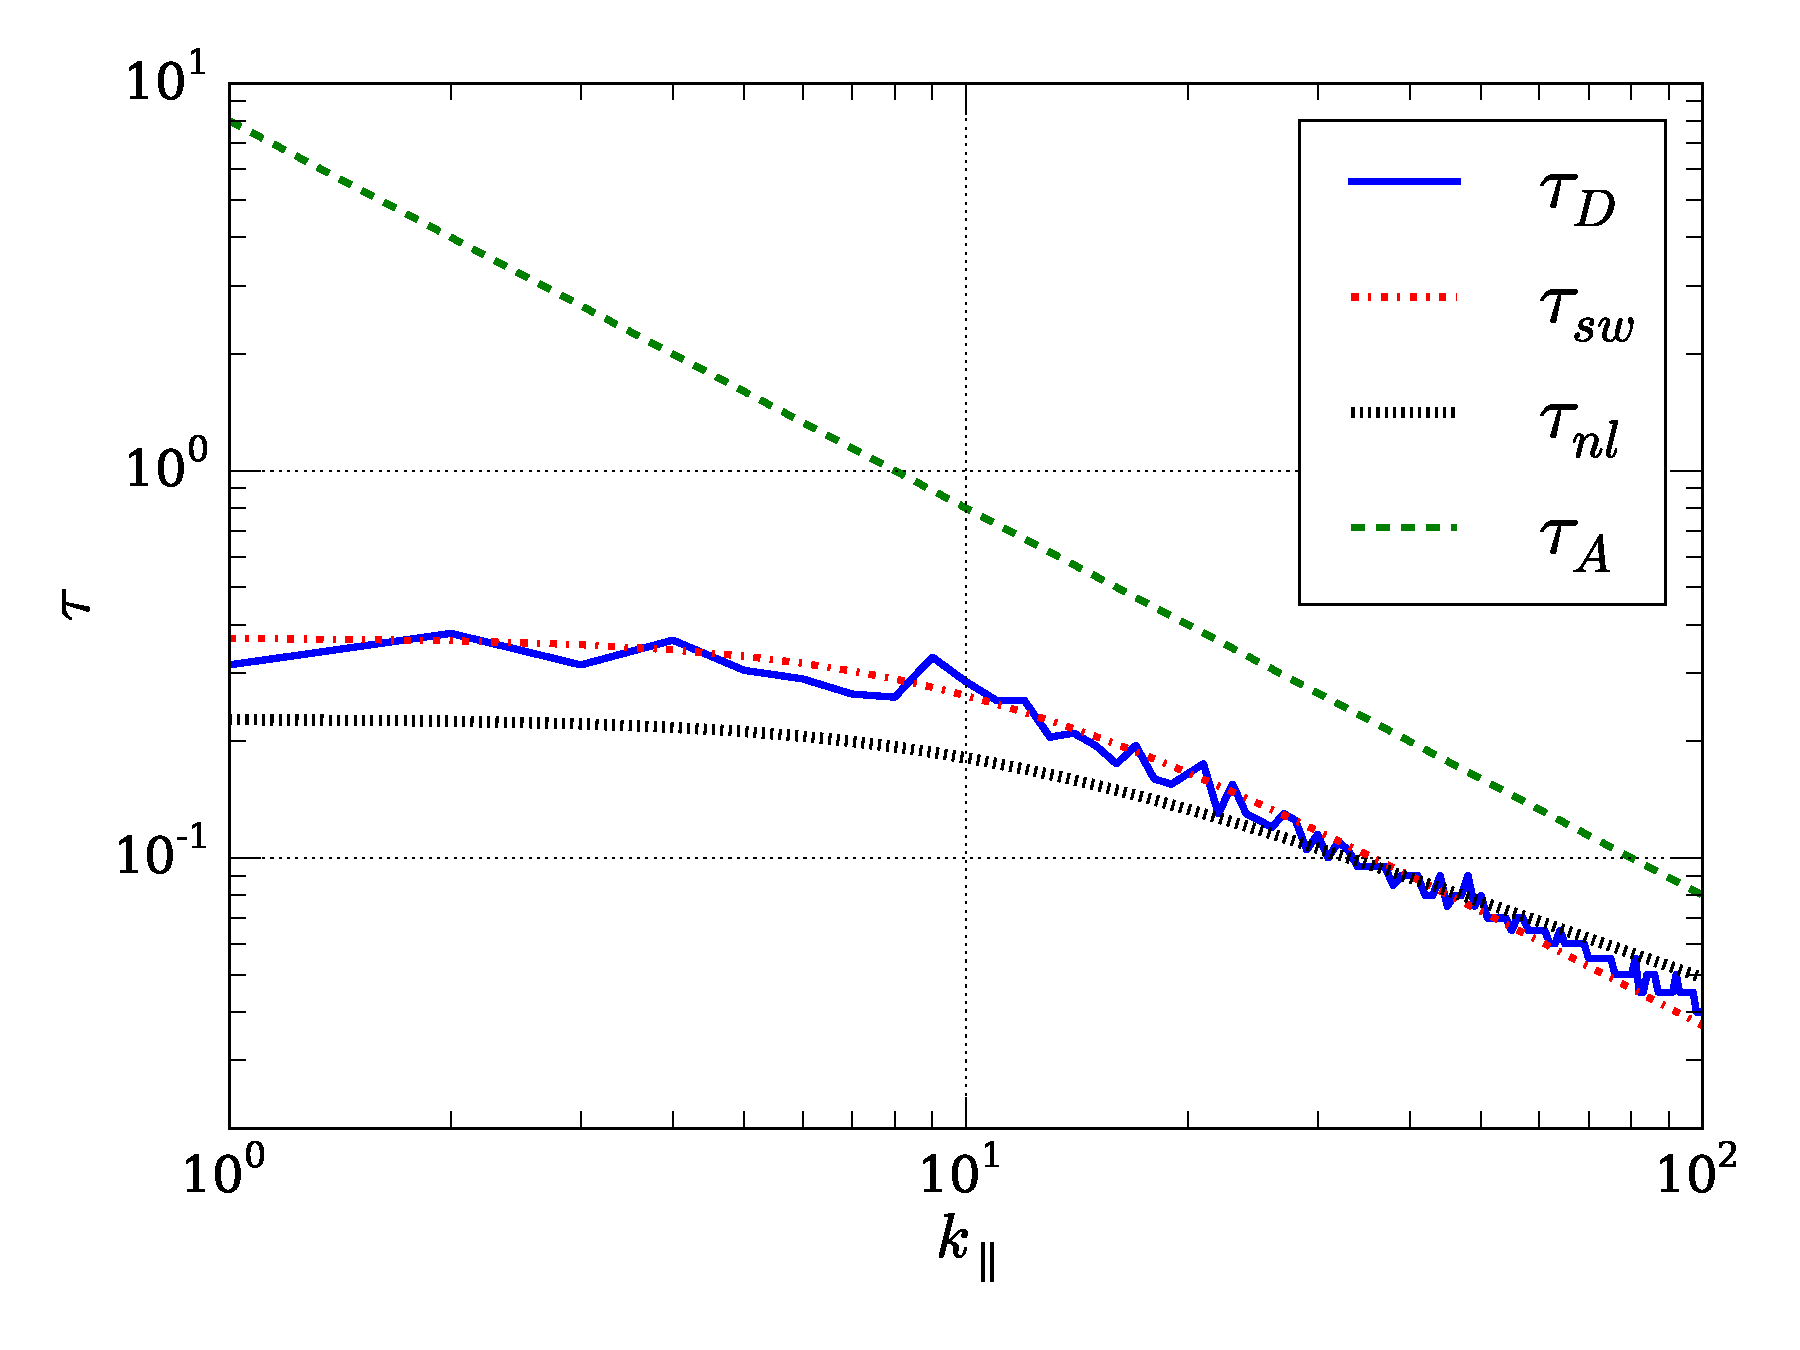
\includegraphics[width=1\columnwidth]{SpatioTemporalSpectra/fig5_B025_b_kperp_10-eps-converted-to.pdf}}

  \subfigure[$k_\perp=20$]{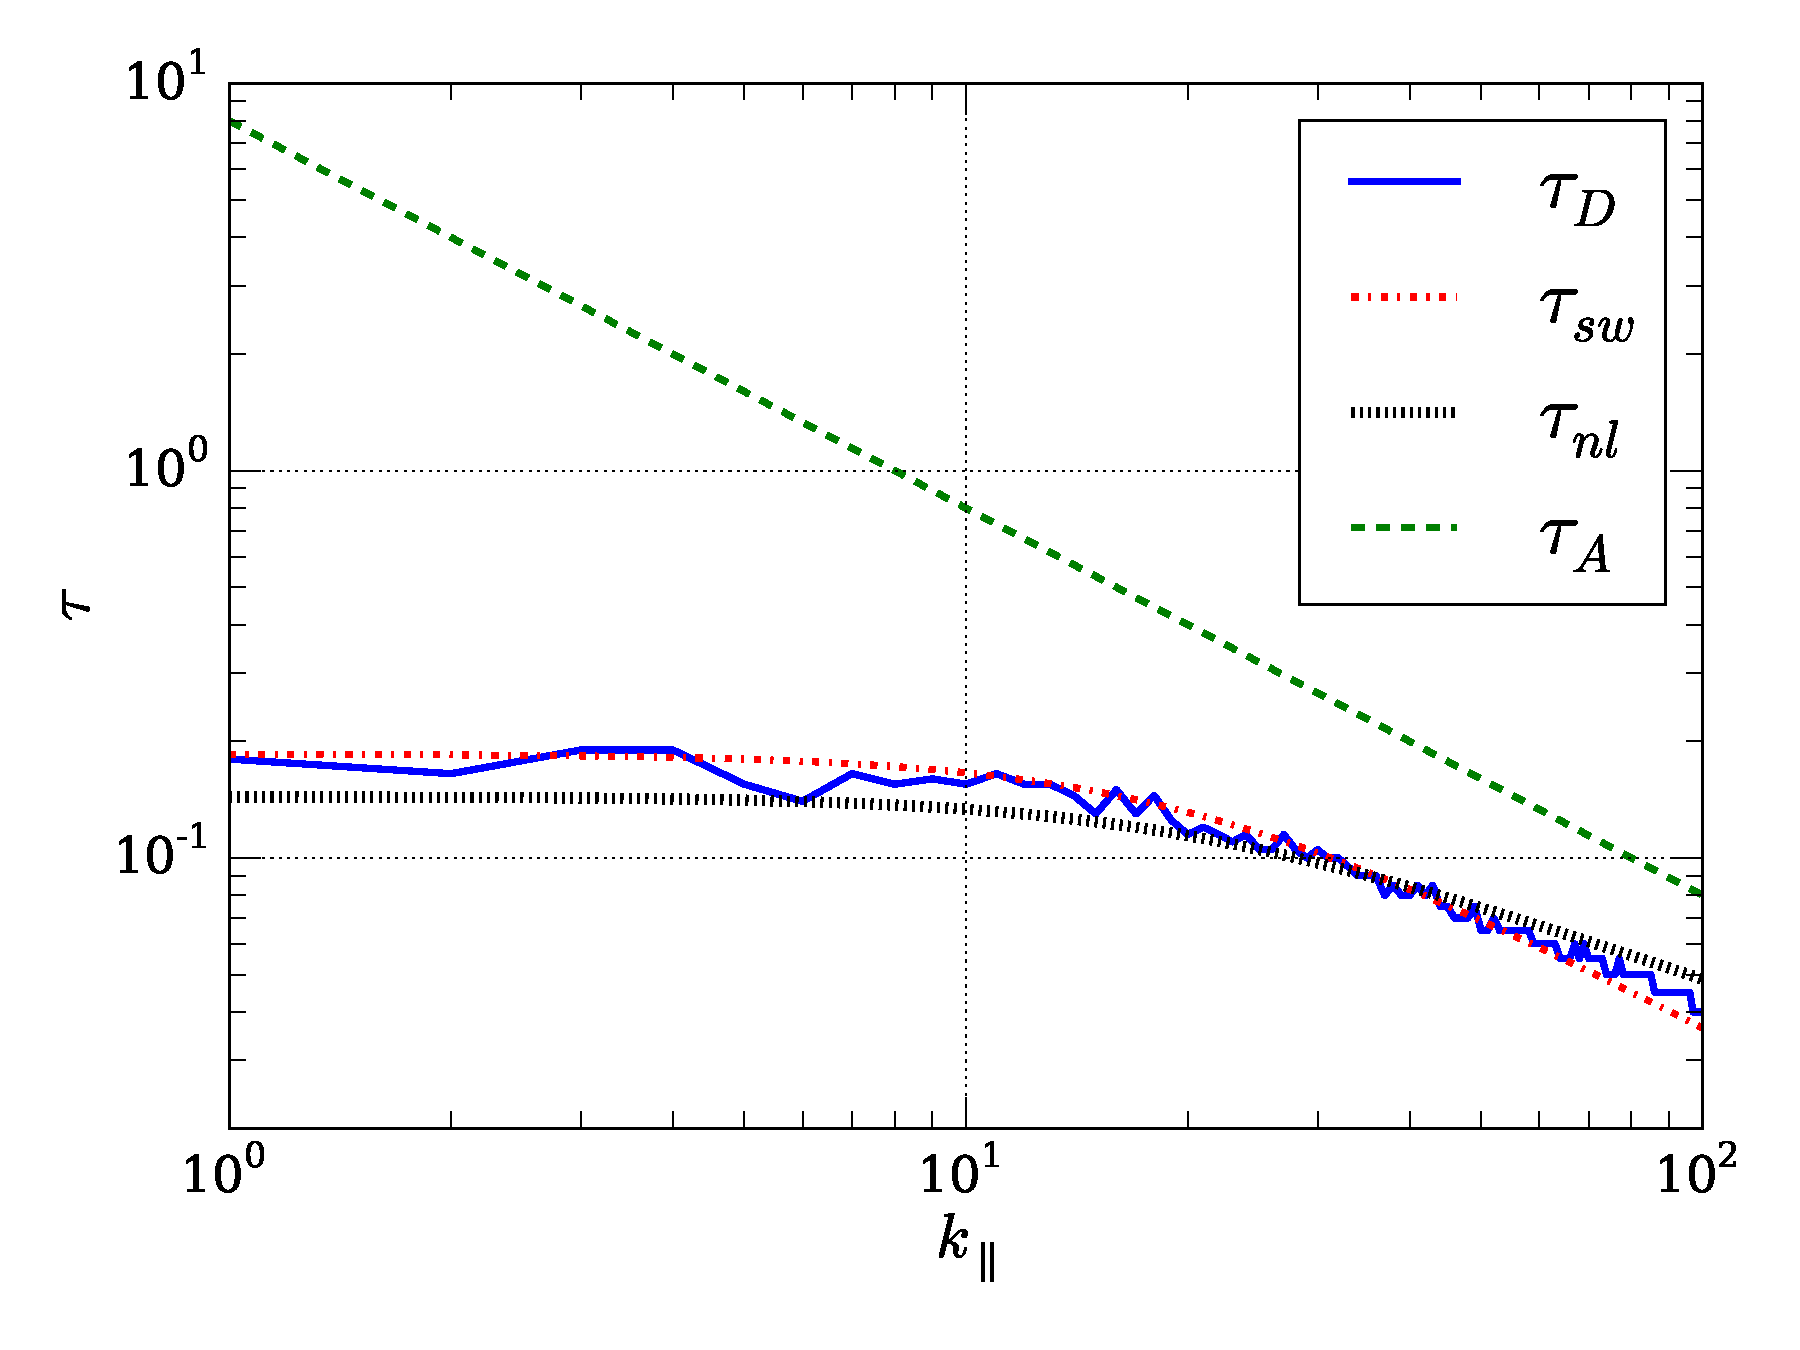
\includegraphics[width=1\columnwidth]{SpatioTemporalSpectra/fig5_B025_b_kperp_20-eps-converted-to.pdf}}
  \caption{Decorrelation times $\tau_D$ for the run with 
    $B_0=0.25$. In each panel $k_\perp$ is held constant and $k_\parallel$
    is varied; (a) $k_\perp = 0$, (b) $k_\perp = 10$, and (c) $k_\perp =
    20$. The lines indicate theoretical predictions for the scaling of
    several physical time scales. The measured value of $\tau_D$ is always
    close to $\tau_{sw}$, except for $k_\perp = 0$ and $k_\parallel$
    between $\approx 1$ and 5 for which the dominant time scale is the
    Alfv\'en time.}
  \label{fig5:B025_bvf_b_kperp}
\end{figure}

\begin{figure}
  \centering
  \subfigure[$k_\parallel=0$]{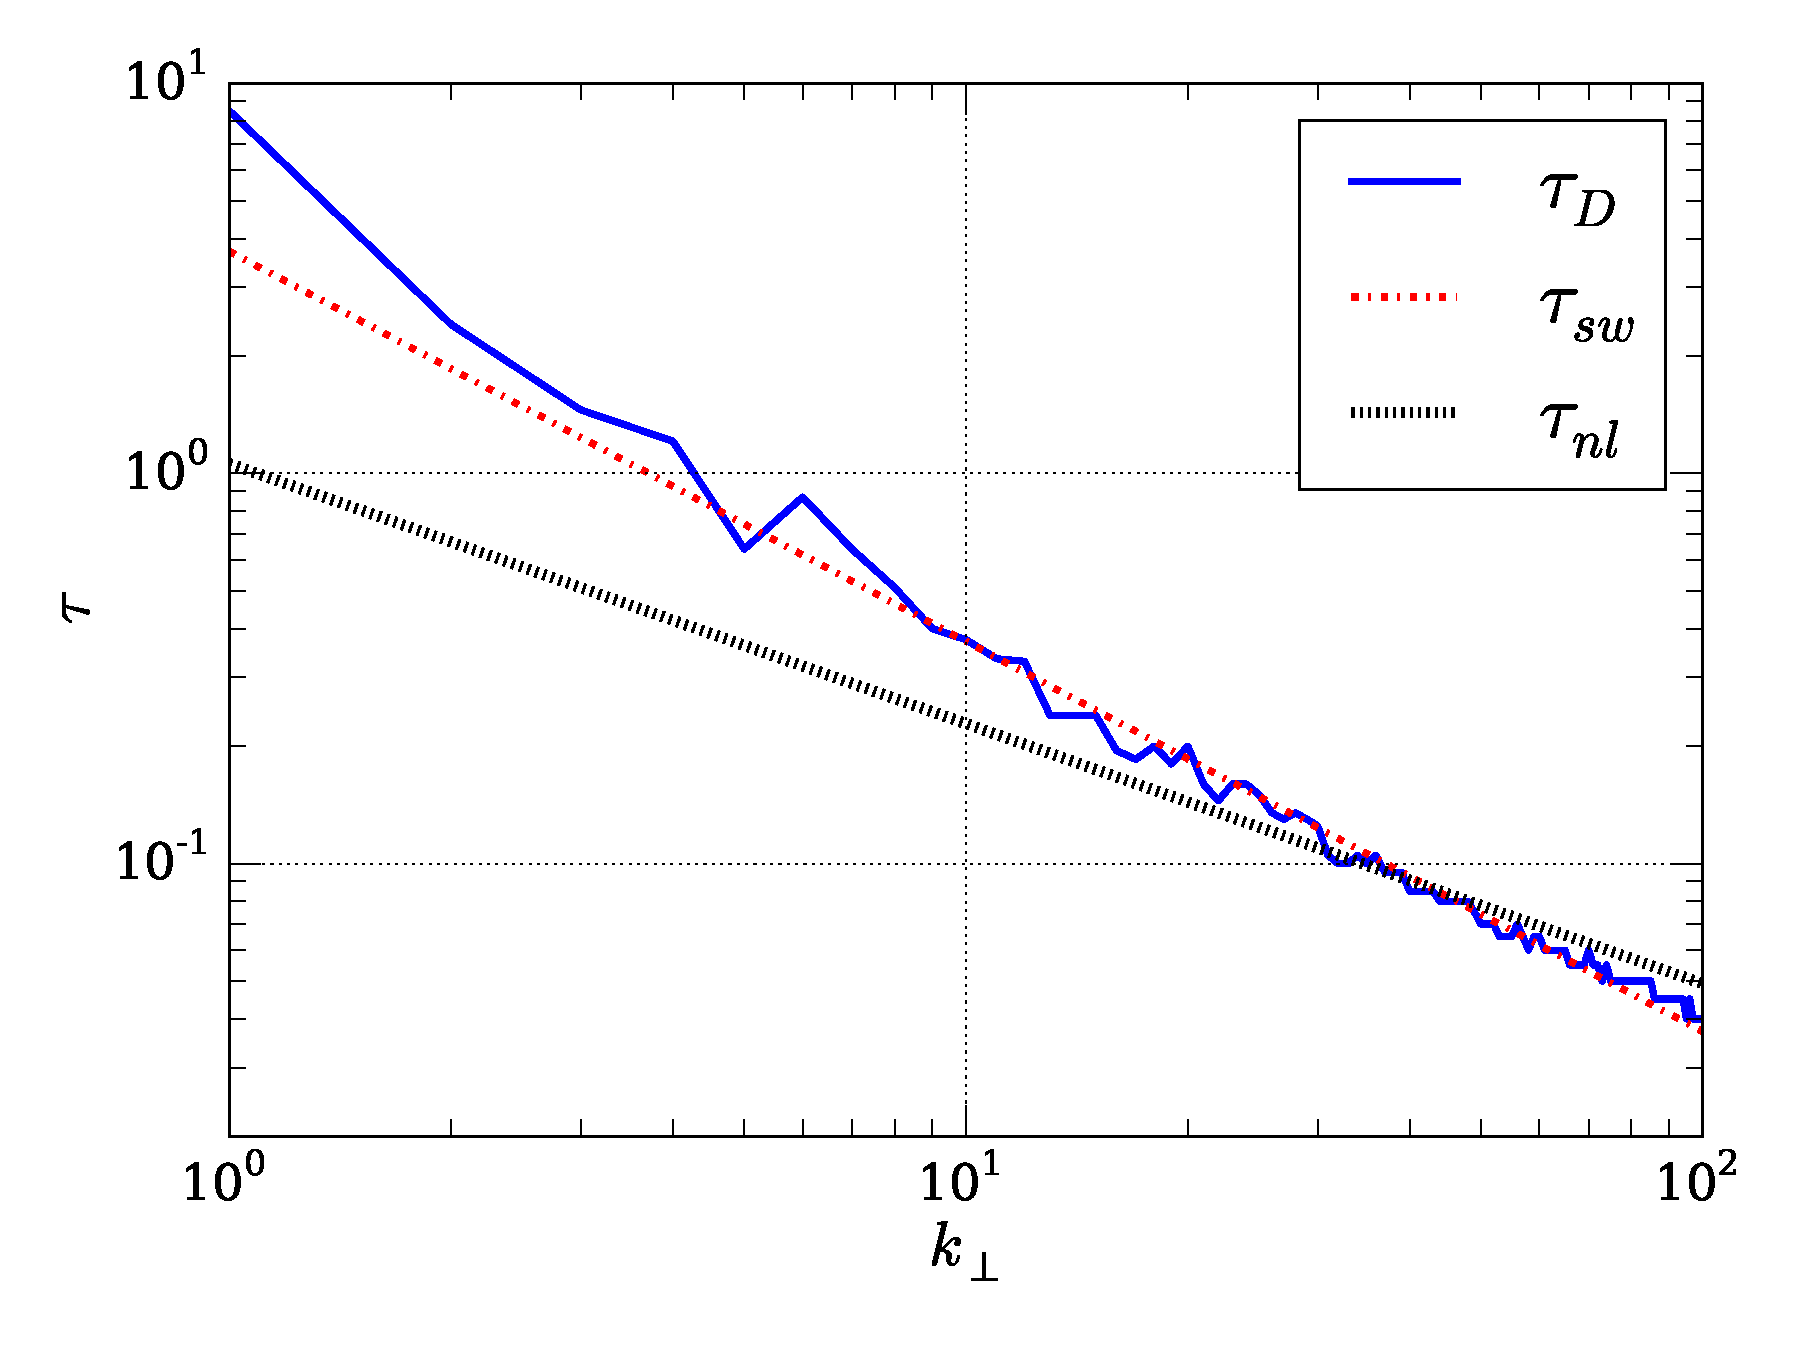
\includegraphics[width=1\columnwidth]{SpatioTemporalSpectra/fig5_B025_b_kpara_0-eps-converted-to.pdf}}

  \subfigure[$k_\parallel=10$]{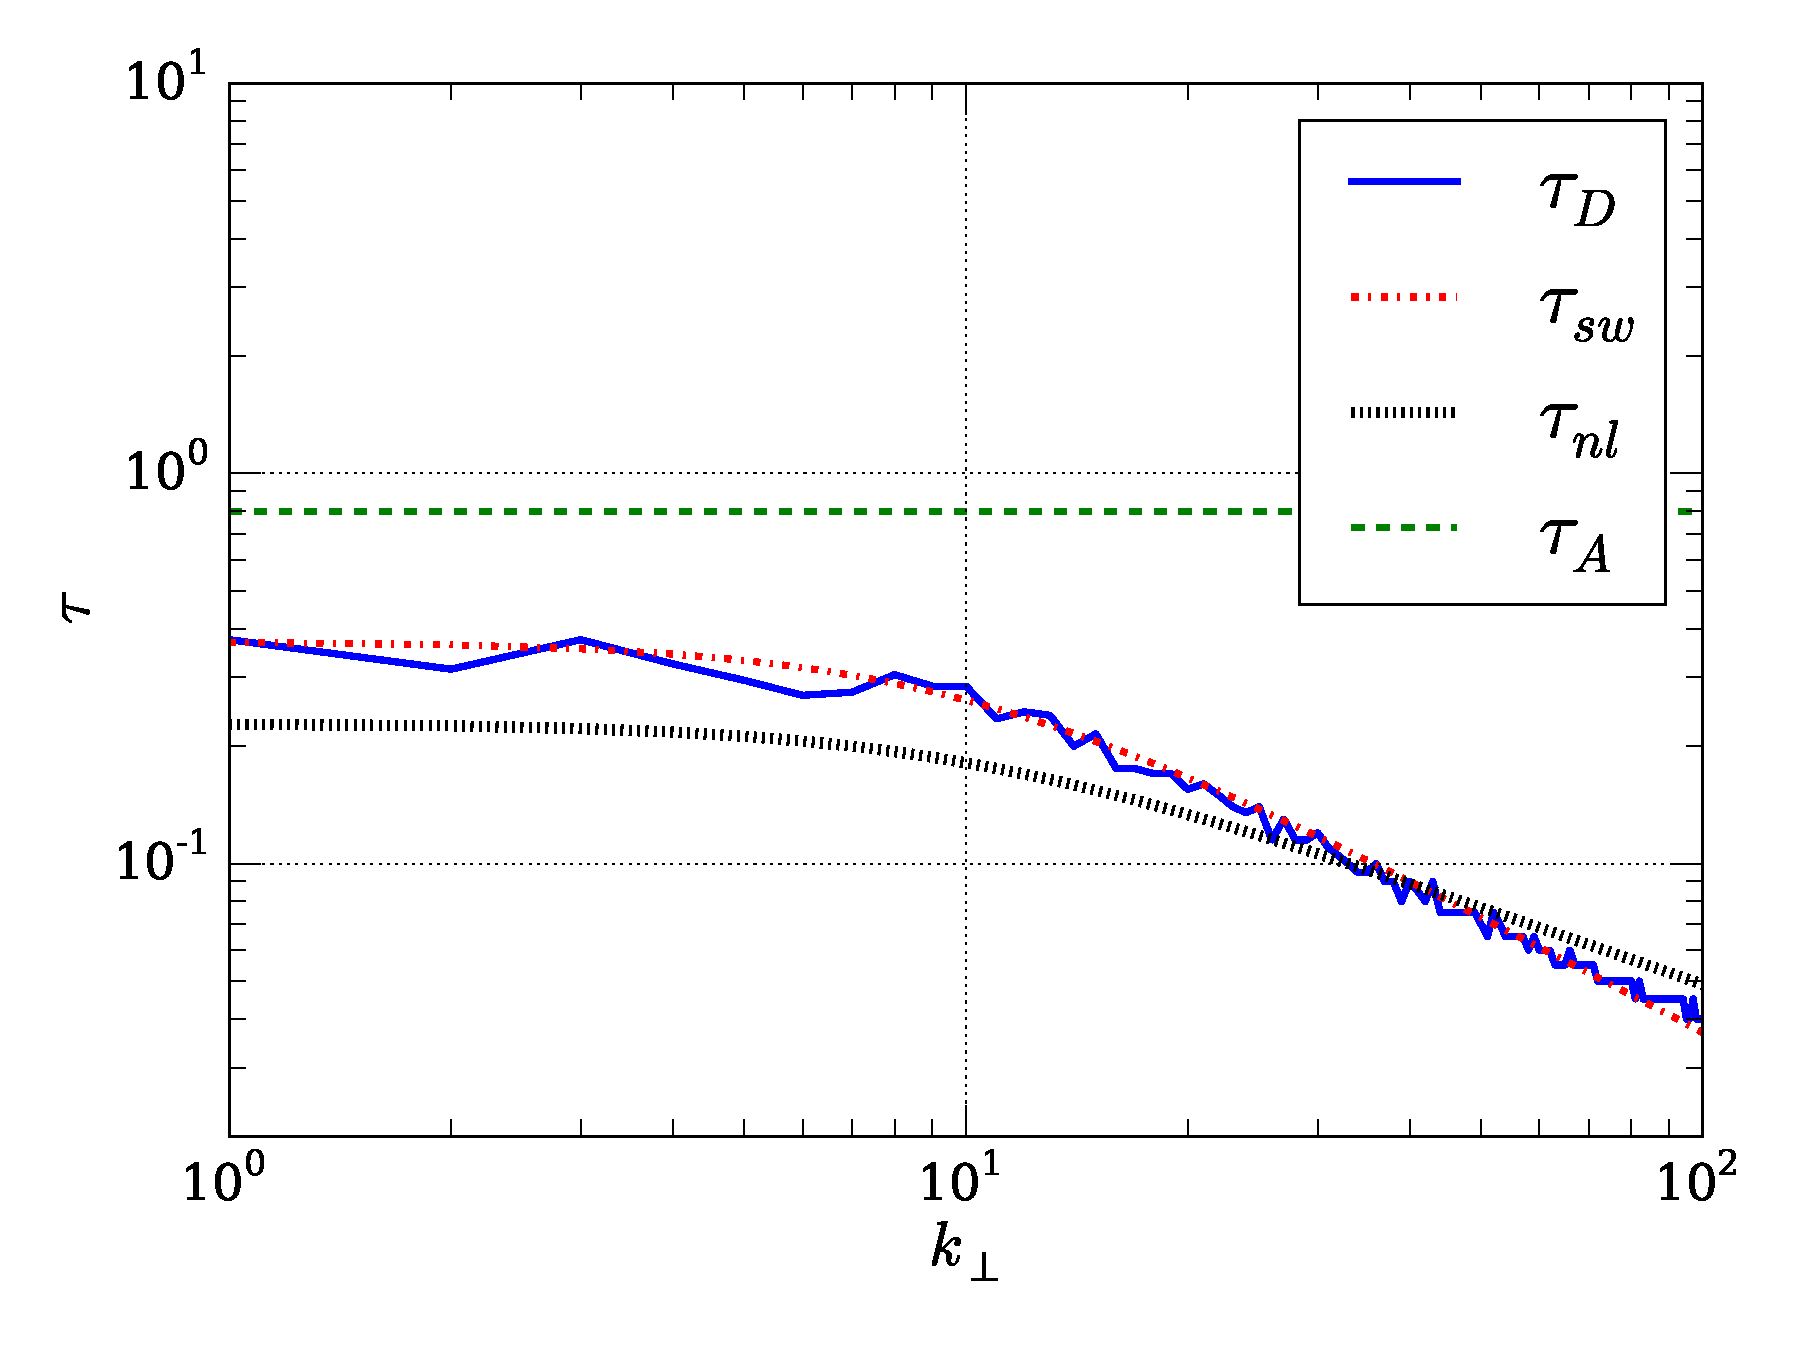
\includegraphics[width=1\columnwidth]{SpatioTemporalSpectra/fig5_B025_b_kpara_10-eps-converted-to.pdf}}

  \subfigure[$k_\parallel=20$]{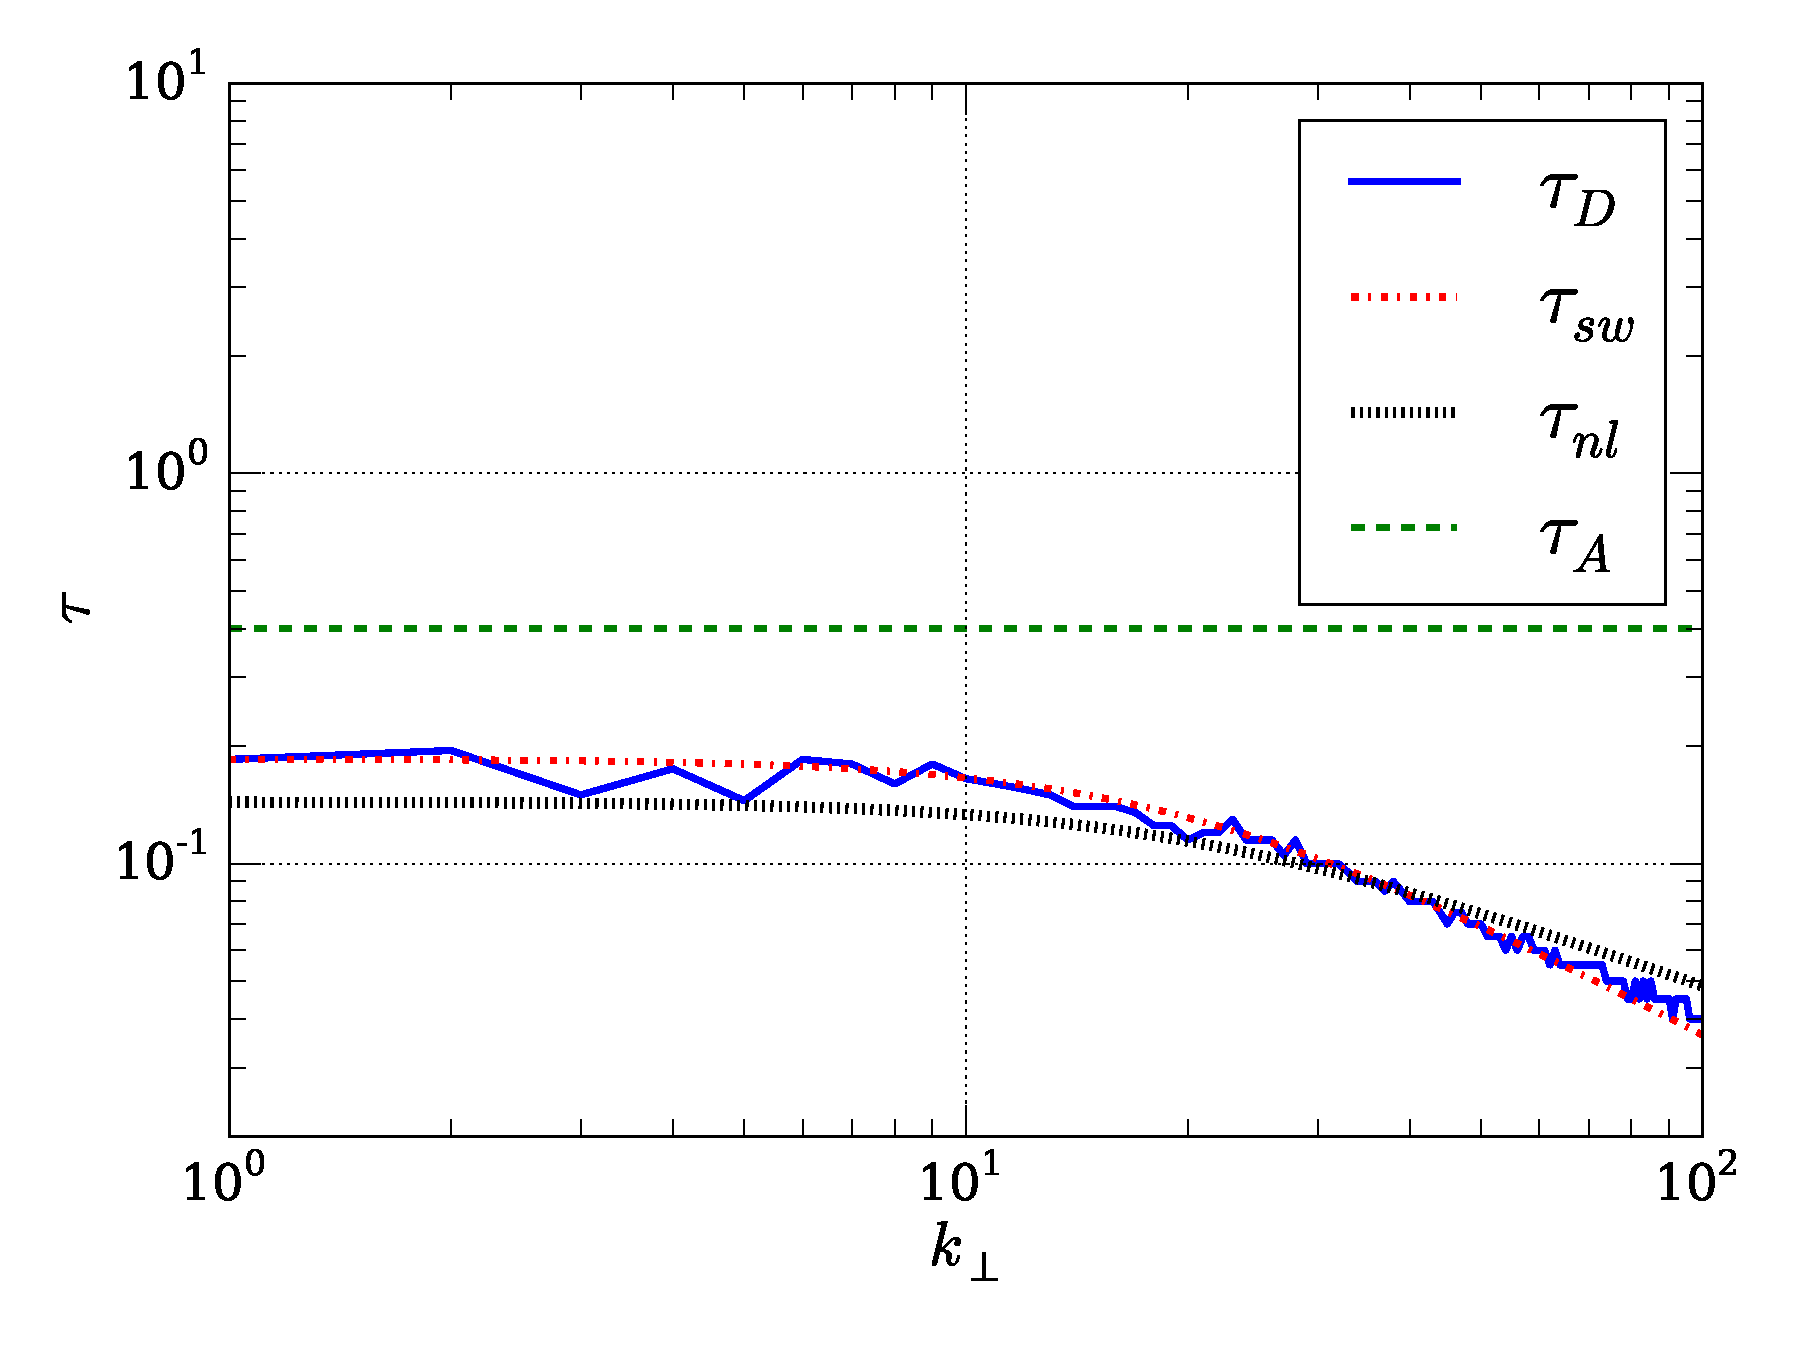
\includegraphics[width=1\columnwidth]{SpatioTemporalSpectra/fig5_B025_b_kpara_20-eps-converted-to.pdf}}
  \caption{Decorrelation times $\tau_D$ for the run with
    $B_0=0.25$. In each panel $k_\parallel$ is held constant and
    $k_\perp$ is varied; (a) $k_\parallel = 0$, (b) $k_\parallel =
    10$, and (c) $k_\parallel = 20$. The straight lines indicate 
    theoretical predictions for the scaling of the relevant physical time
    scales. The measured value of $\tau_D$ is always close to
    $\tau_{sw}$.}
  \label{fig5:B025_bvf_b_kpara}
\end{figure}

\begin{figure}
  \centering
  \subfigure[$k_\perp=0$]{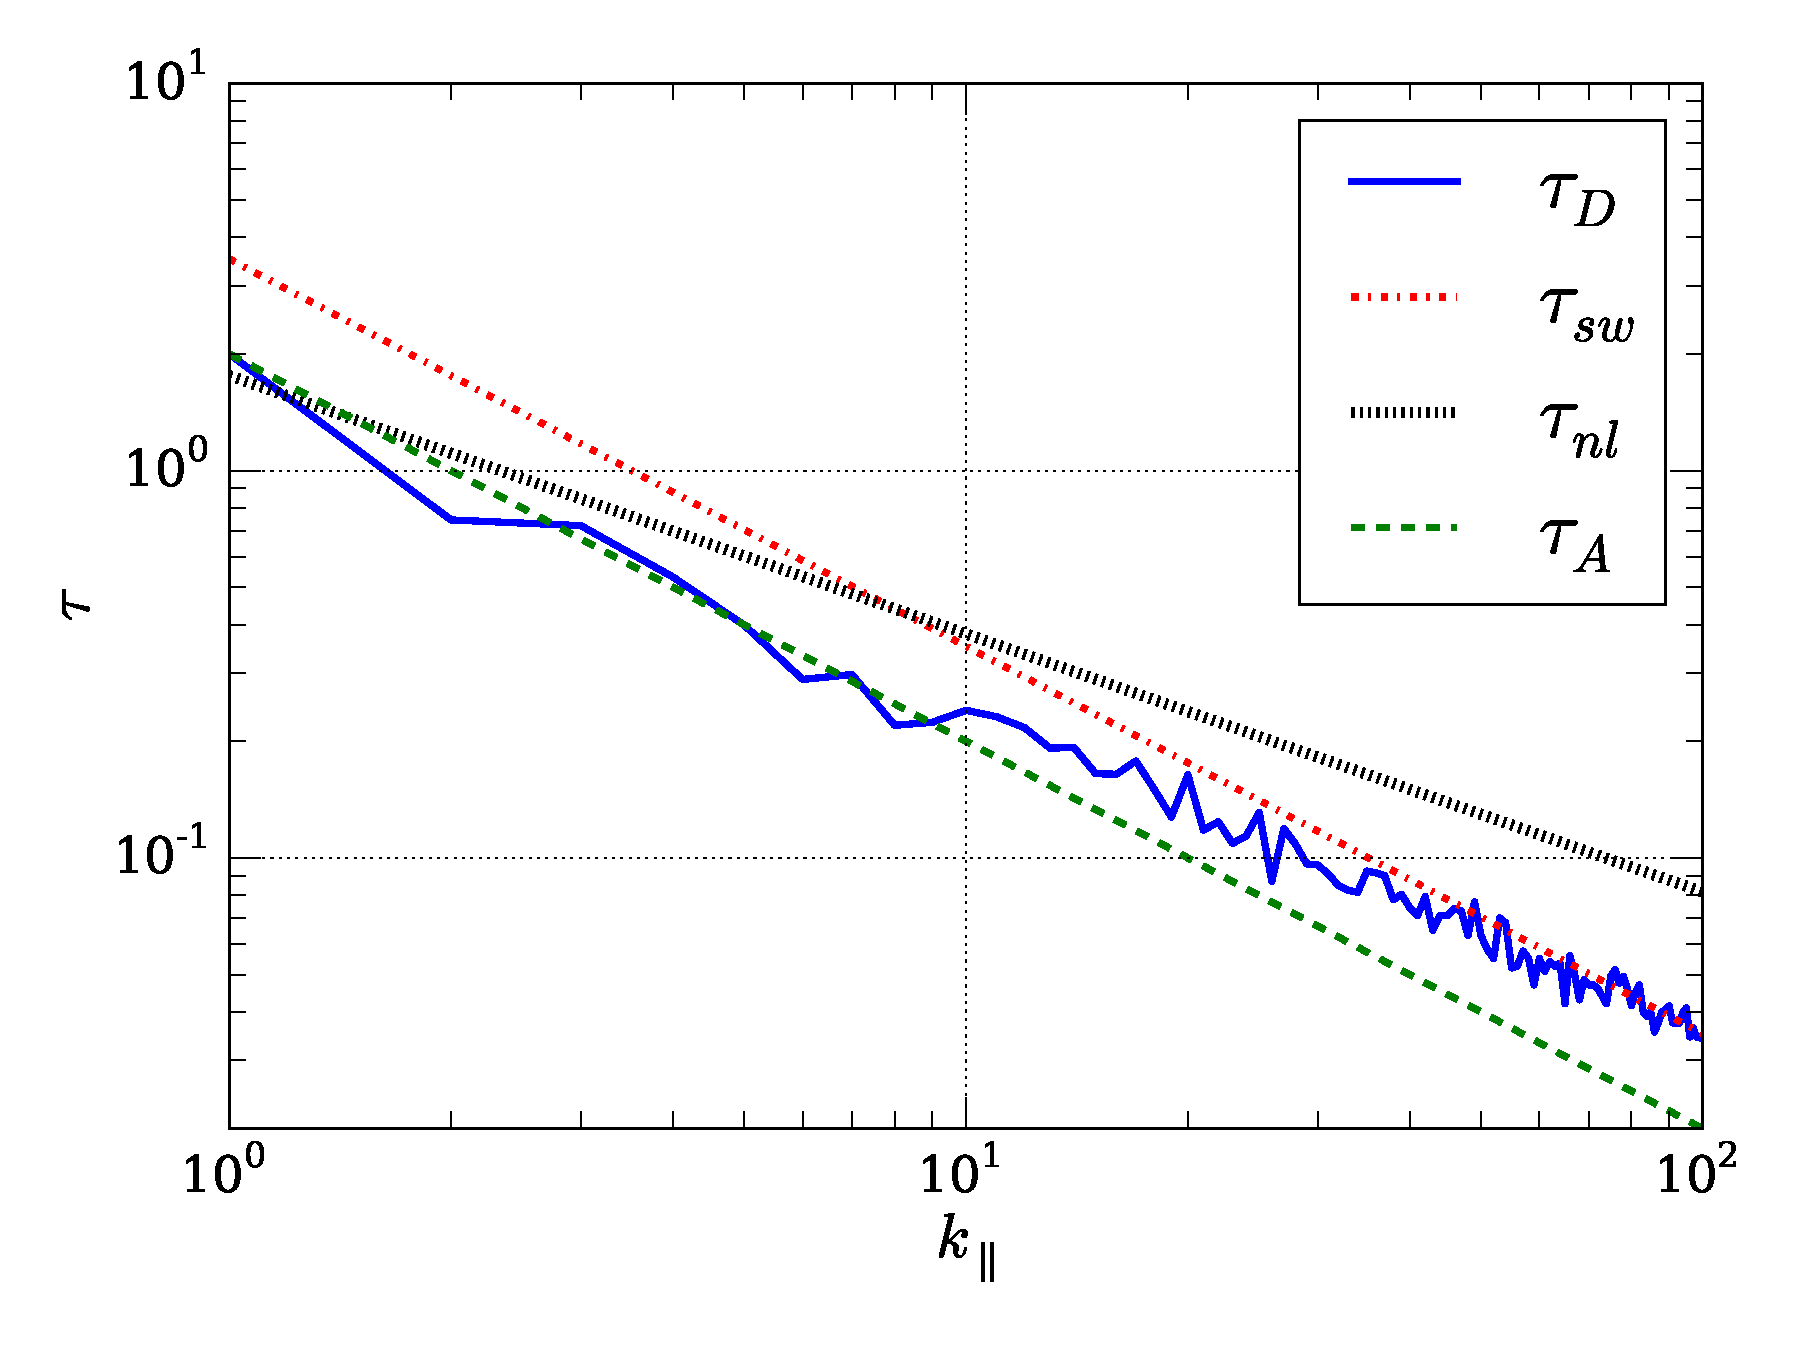
\includegraphics[width=1\columnwidth]{SpatioTemporalSpectra/fig5_B1_b_kperp_0-eps-converted-to.pdf}}

  \subfigure[$k_\perp=10$]{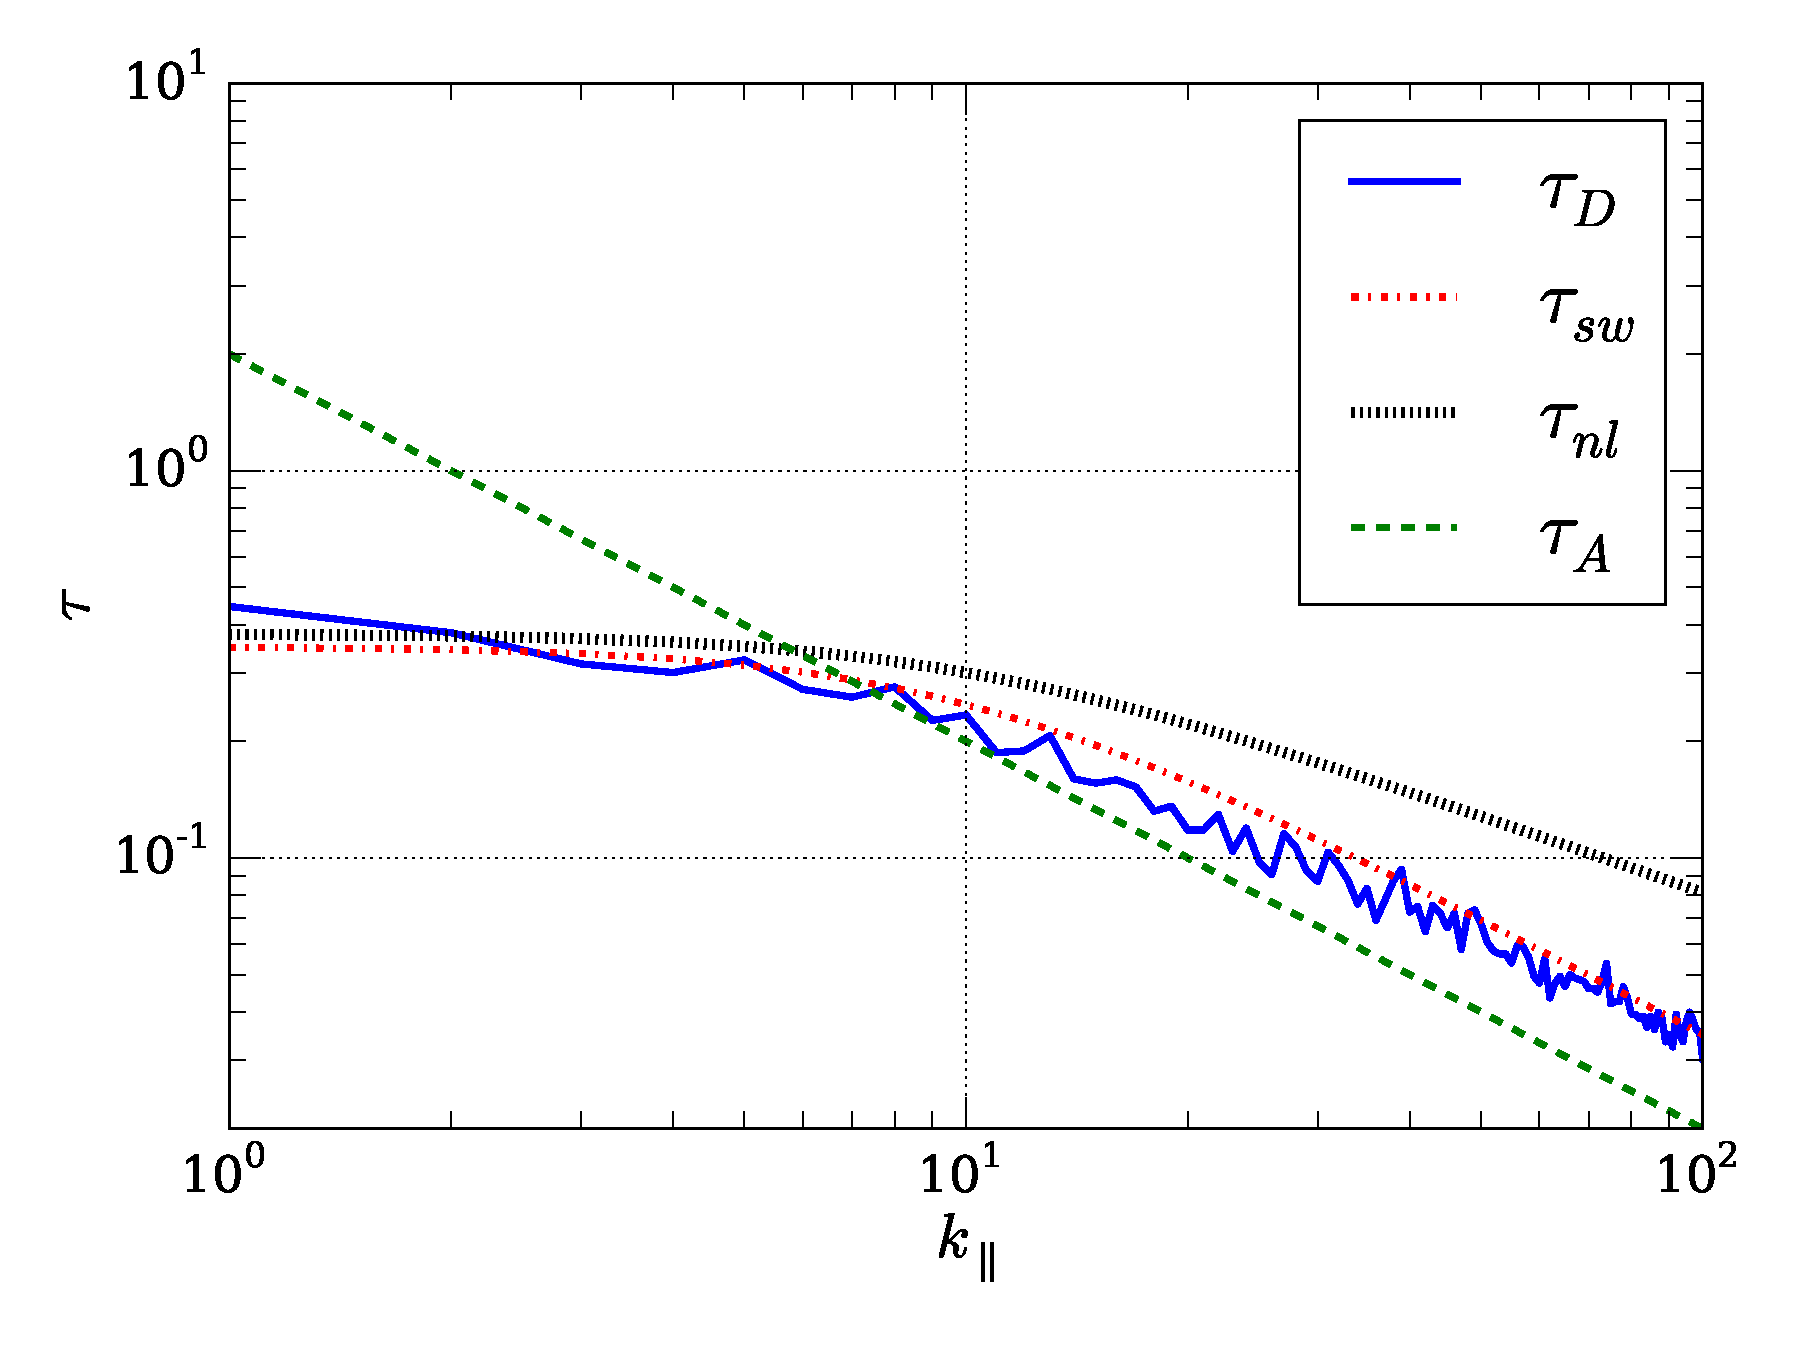
\includegraphics[width=1\columnwidth]{SpatioTemporalSpectra/fig5_B1_b_kperp_10-eps-converted-to.pdf}}

  \subfigure[$k_\perp=20$]{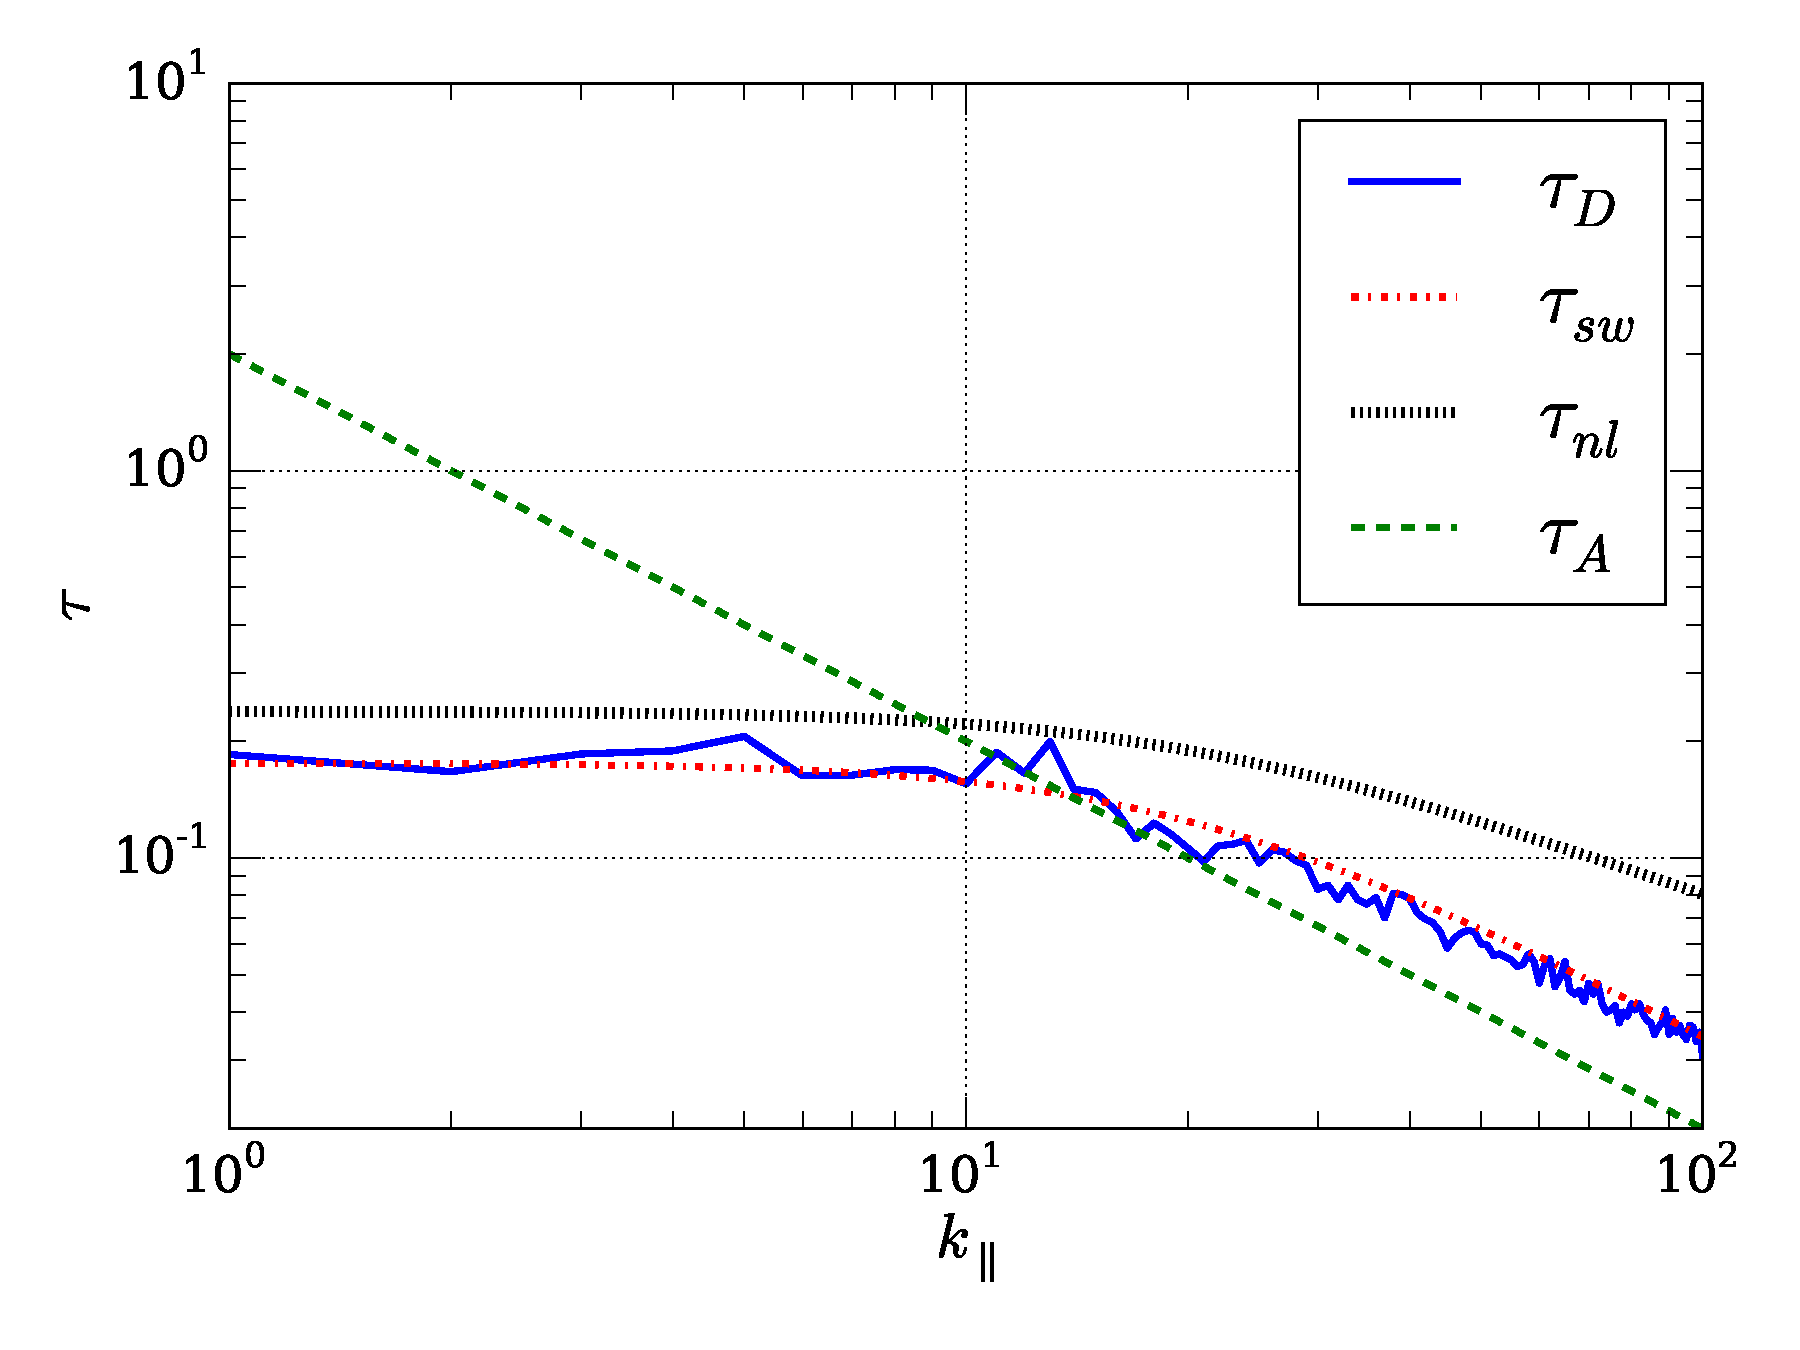
\includegraphics[width=1\columnwidth]{SpatioTemporalSpectra/fig5_B1_b_kperp_20-eps-converted-to.pdf}}
  \caption{Decorrelation times $\tau_D$ for the run with $B_0=1$. In each
    panel $k_\perp$ is held constant and $k_\parallel$ is varied; (a)
    $k_\perp=0$, (b) $k_\perp = 10$, and (c) $k_\perp = 20$. The
    straight lines indicate theoretical predictions for
    the scaling of the relevant physical time scales.}
  \label{fig5:B1_bvf_b_kperp}
\end{figure}

\begin{figure}
  \centering
  \subfigure[$k_\parallel=0$]{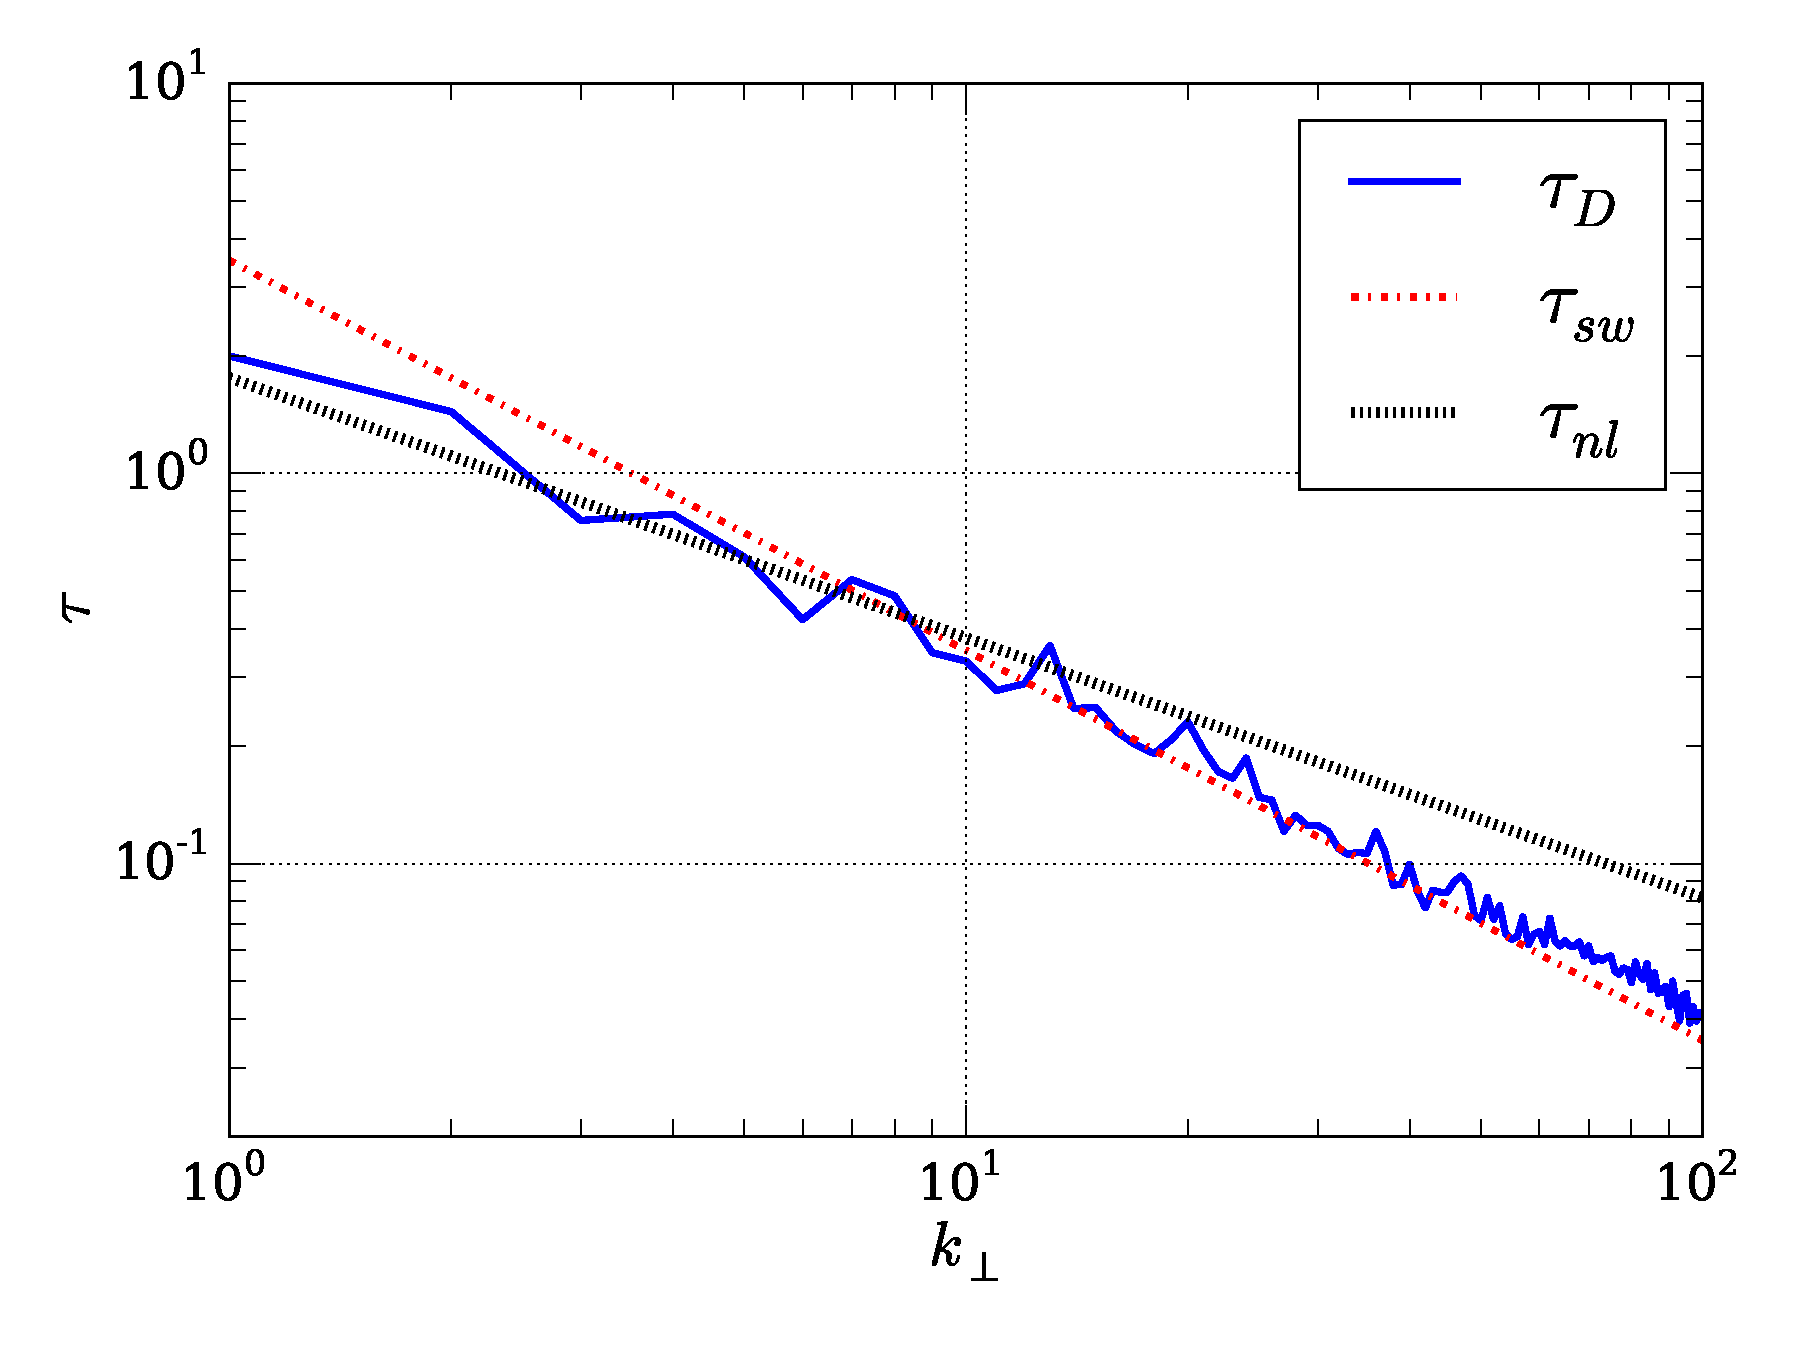
\includegraphics[width=1\columnwidth]{SpatioTemporalSpectra/fig5_B1_b_kpara_0-eps-converted-to.pdf}}

  \subfigure[$k_\parallel=10$]{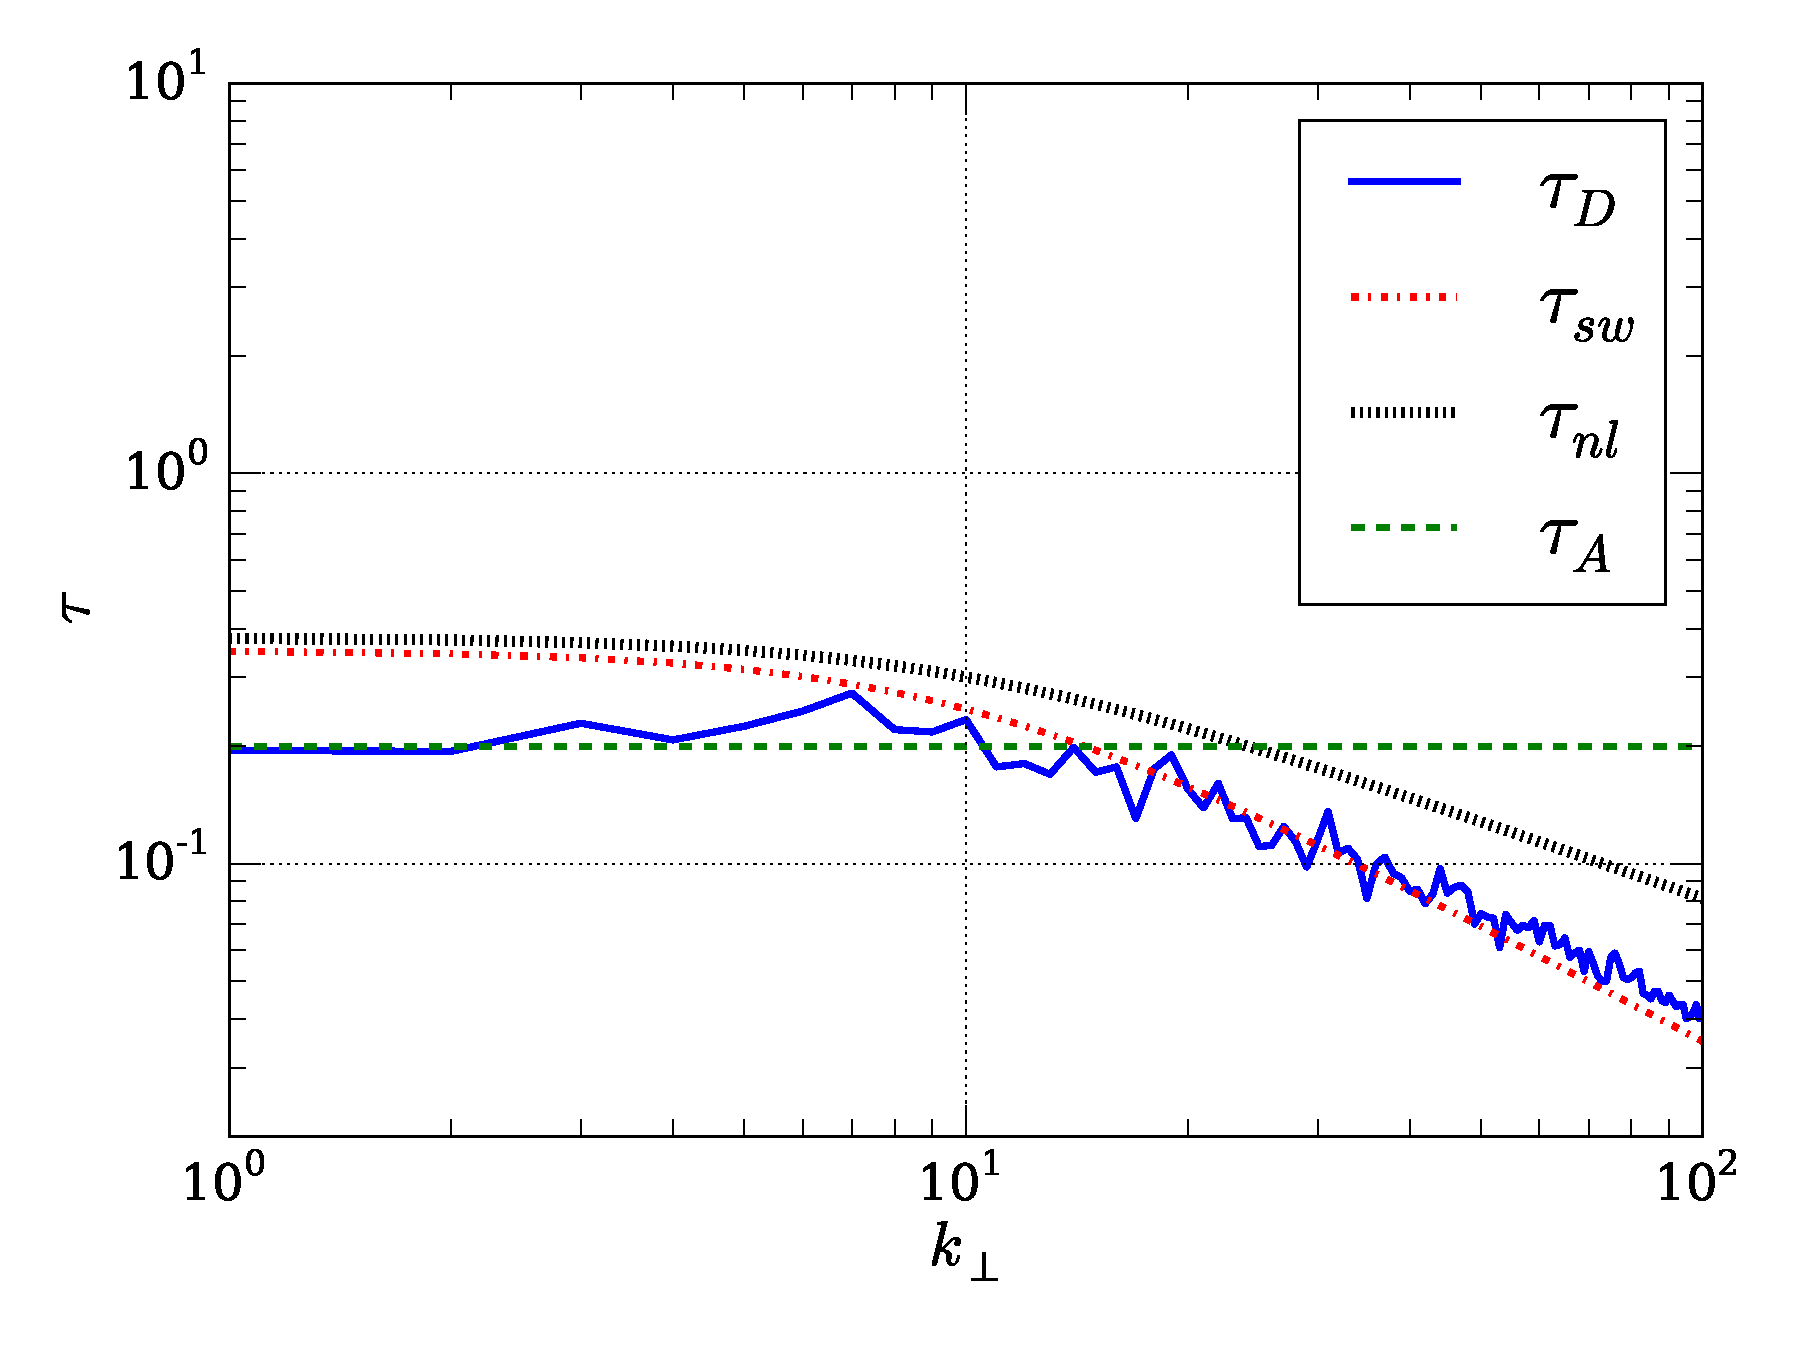
\includegraphics[width=1\columnwidth]{SpatioTemporalSpectra/fig5_B1_b_kpara_10-eps-converted-to.pdf}}

  \subfigure[$k_\parallel=20$]{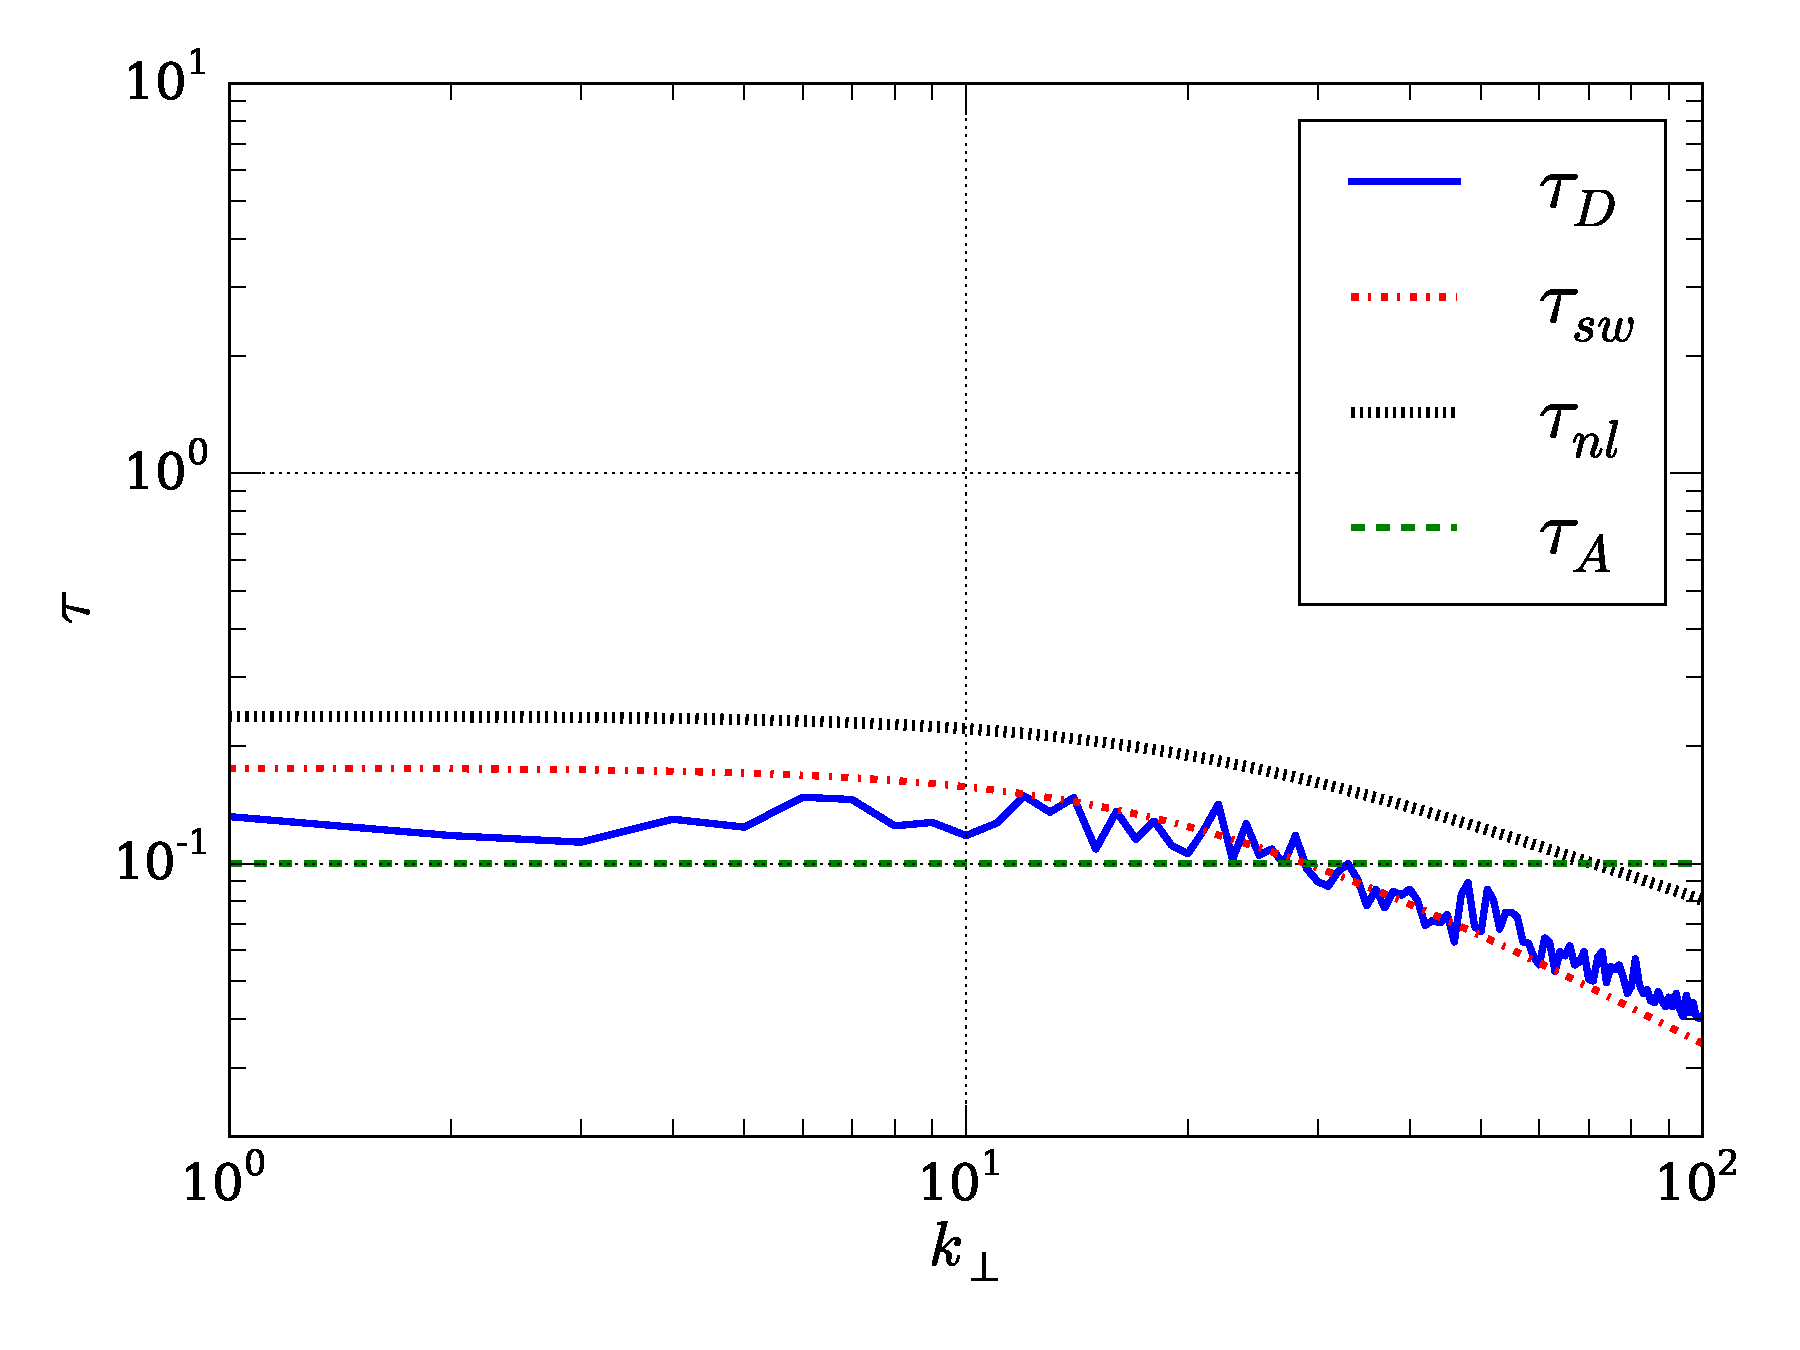
\includegraphics[width=1\columnwidth]{SpatioTemporalSpectra/fig5_B1_b_kpara_20-eps-converted-to.pdf}}
  \caption{Decorrelation times $\tau_D$ for the run with $B_0=1$. In each
    panel $k_\parallel$ is held constant and $k_\perp$ is varied; (a)
    $k_\parallel = 0$, (b) $k_\parallel = 10$, and (c) $k_\parallel =
    20$. The straight lines indicate theoretical predictions for
    the scaling of the relevant physical time scales.}
  \label{fig5:B1_bvf_b_kpara}
\end{figure}

Finalmente, analicemos el comportamiento del tiempo de descorrelación
$\tau$ para las corridas con el mayor campo magnético medio
considerado, $B_0=8$. Los resultados se pueden ver en las
\cref{fig5:B8_bvf_b_kperp, fig5:B8_bvf_b_kpara}. Para valores pequeños
de $k_\perp$, se encuentra que el tiempo de Alfvén resulta dominante
de las descorrelaciones (hasta, aproximadamente, $k_\parallel = 10$;
ver \cref{fig5:B8_bvf_b_kpara}). Para valores mayores de $k_{\perp}$,
sin embargo, el tiempo de descorrelación se aleja del tiempo de Alfvén
y se acerca lentamente a la escala del tiempo de \sweeping. Esto es
consistente con los espectros espacio-temporales de la
\cref{fig3:B8_bvf_Etot_kperp0}, donde se observa que la energía se
concentra cerca de la relación de dispersión de Alfvén para valores
pequeños del número de onda, pero se difumina hacia las frecuencias de
\sweeping para valores grandes del número de onda.  Como resultado, es
la competencia entre estas dos escalas temporales la que parece ser
responsable del ensanchamiento del espectro espacio-temporal para
valores grandes de $B_0$. En tanto el tiempo de Alfvén sea mucho más
rápido que las otras escalas temporales del sistema, el flujo excita
ondas de Alfvén, que dominan los modos de doscorrelación. Pero cuando
las otras escalas se acercan a la escala temporal de las ondas (o
hasta se vuelven más rápidas, como sucede para valores pequeños de
$B_0$), el sistema cambia la escala temporal dominante en la
descorrelación.

\begin{figure}
  \centering
  \subfigure[$k_\perp=0$]{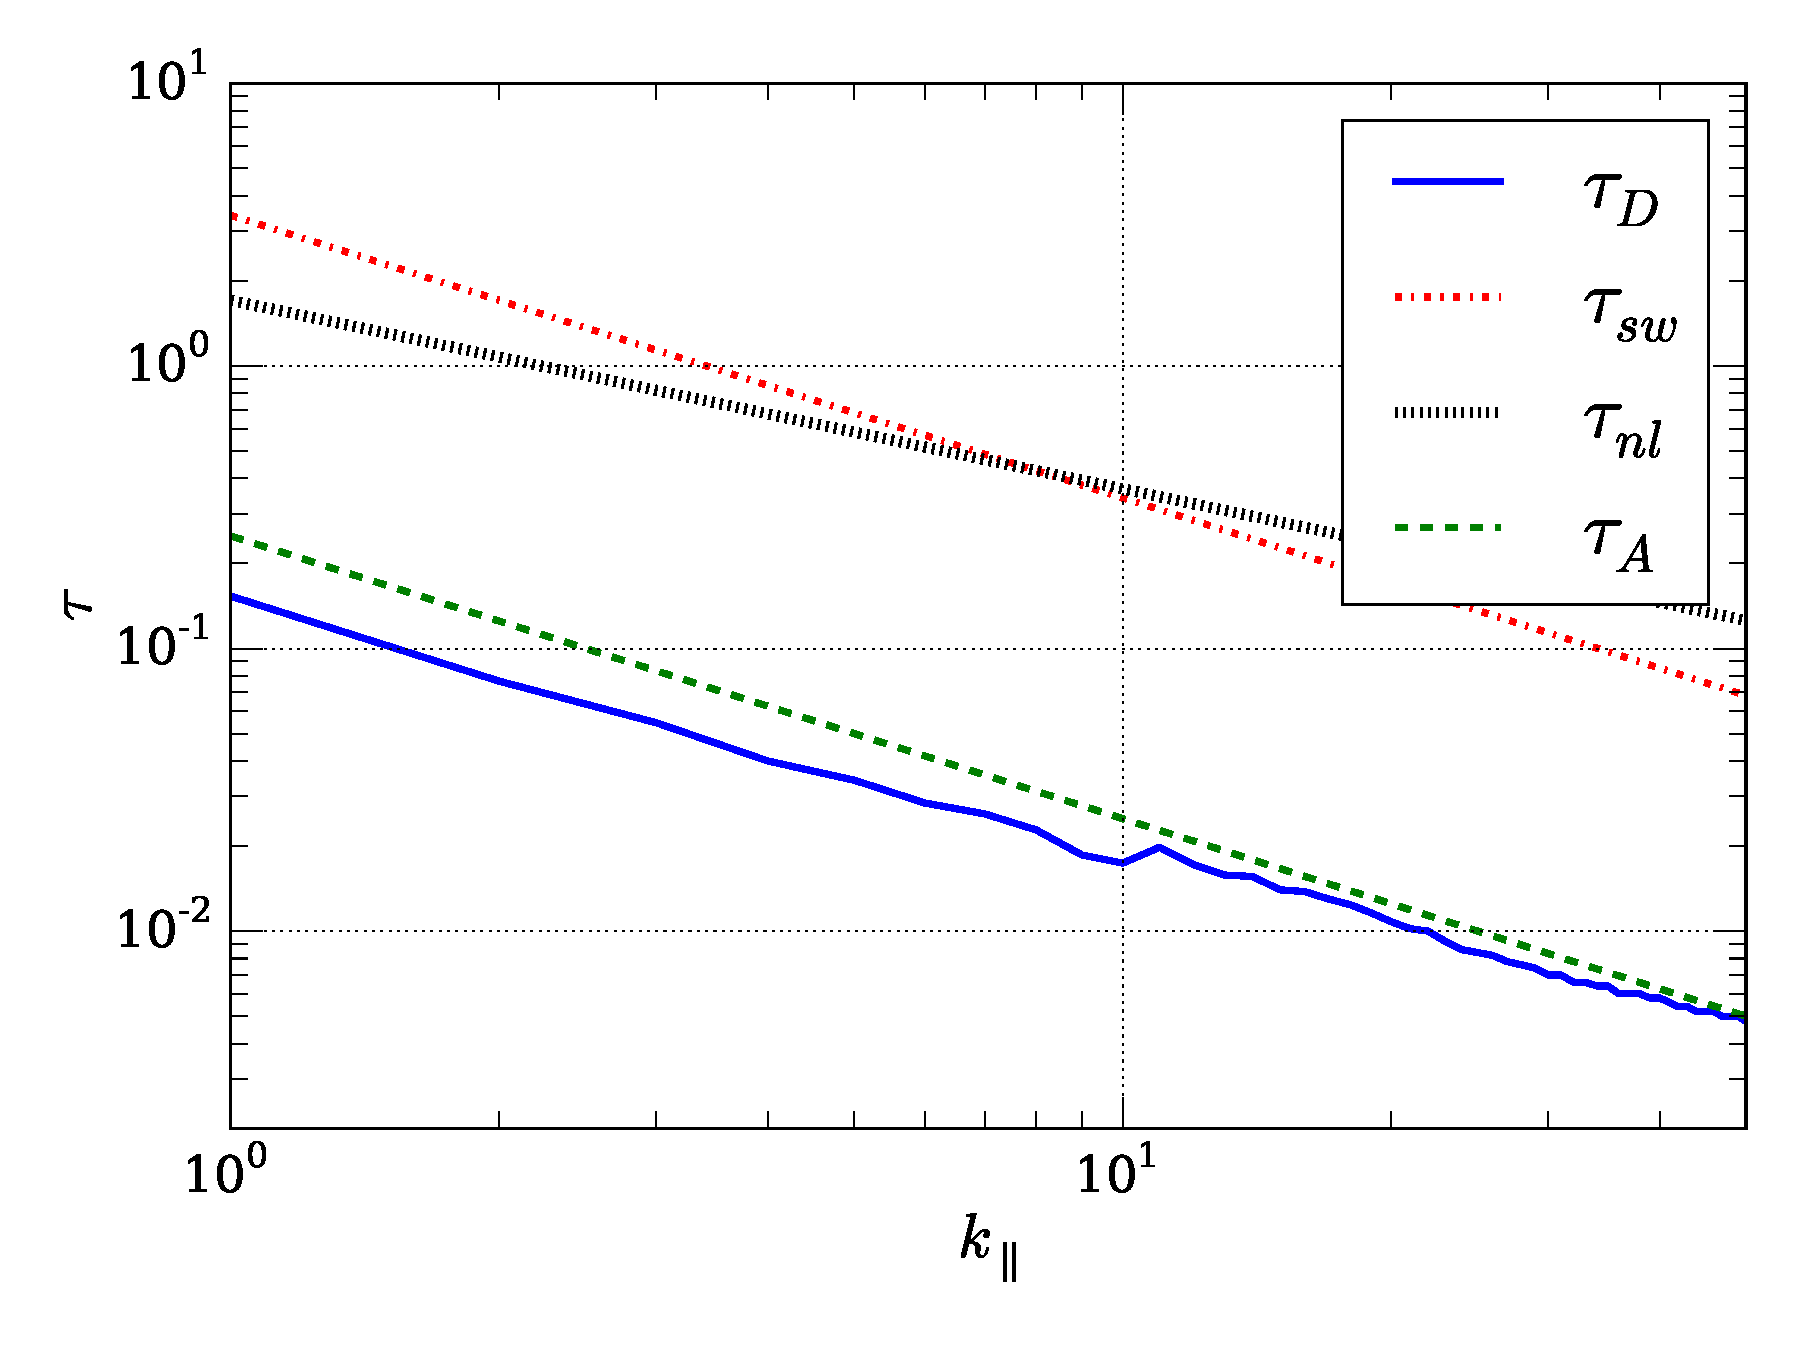
\includegraphics[width=1\columnwidth]{SpatioTemporalSpectra/fig5_B8_b_kperp_0-eps-converted-to.pdf}}

  \subfigure[$k_\perp=10$]{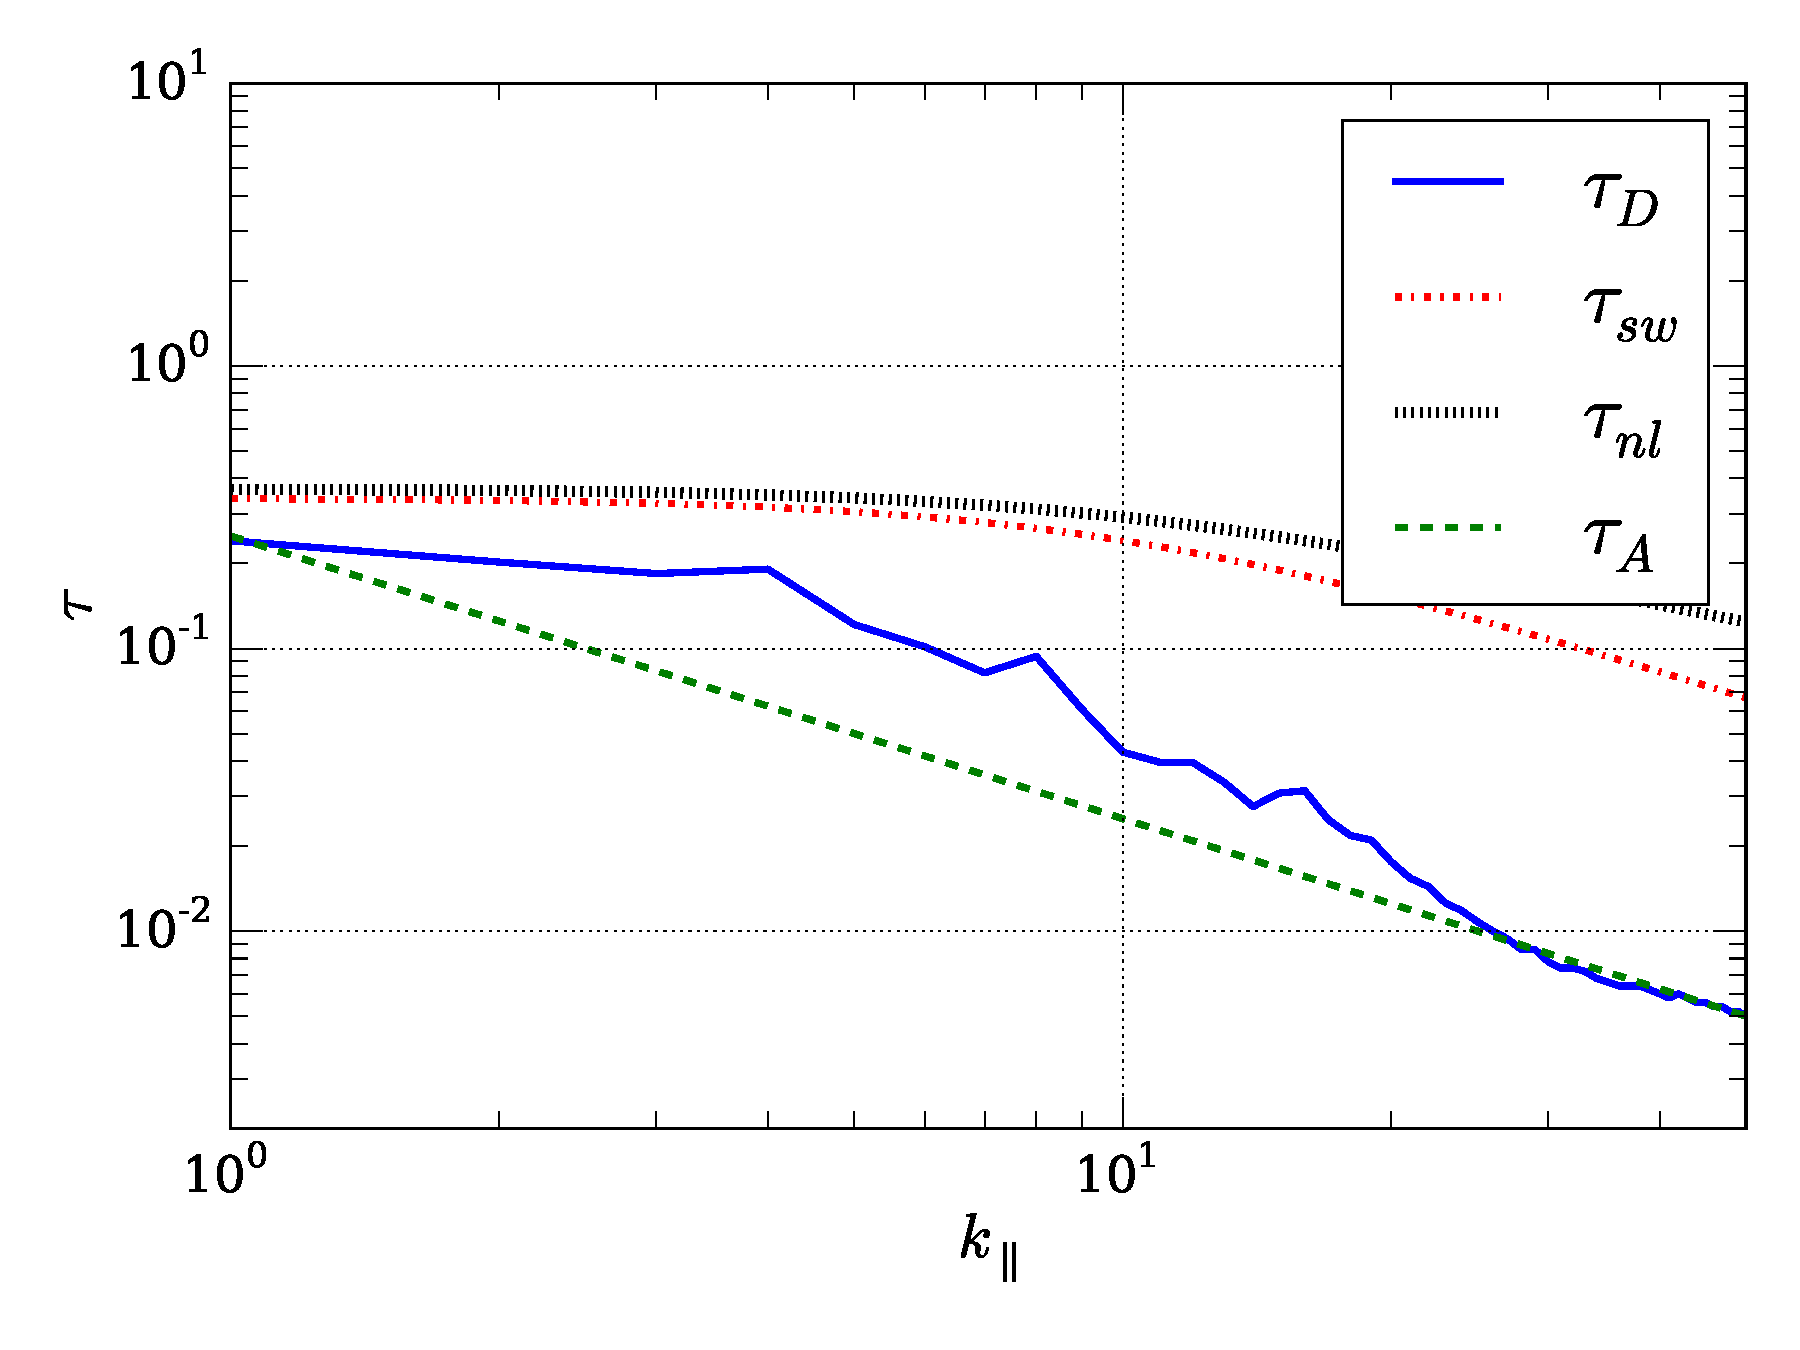
\includegraphics[width=1\columnwidth]{SpatioTemporalSpectra/fig5_B8_b_kperp_10-eps-converted-to.pdf}}

  \subfigure[$k_\perp=20$]{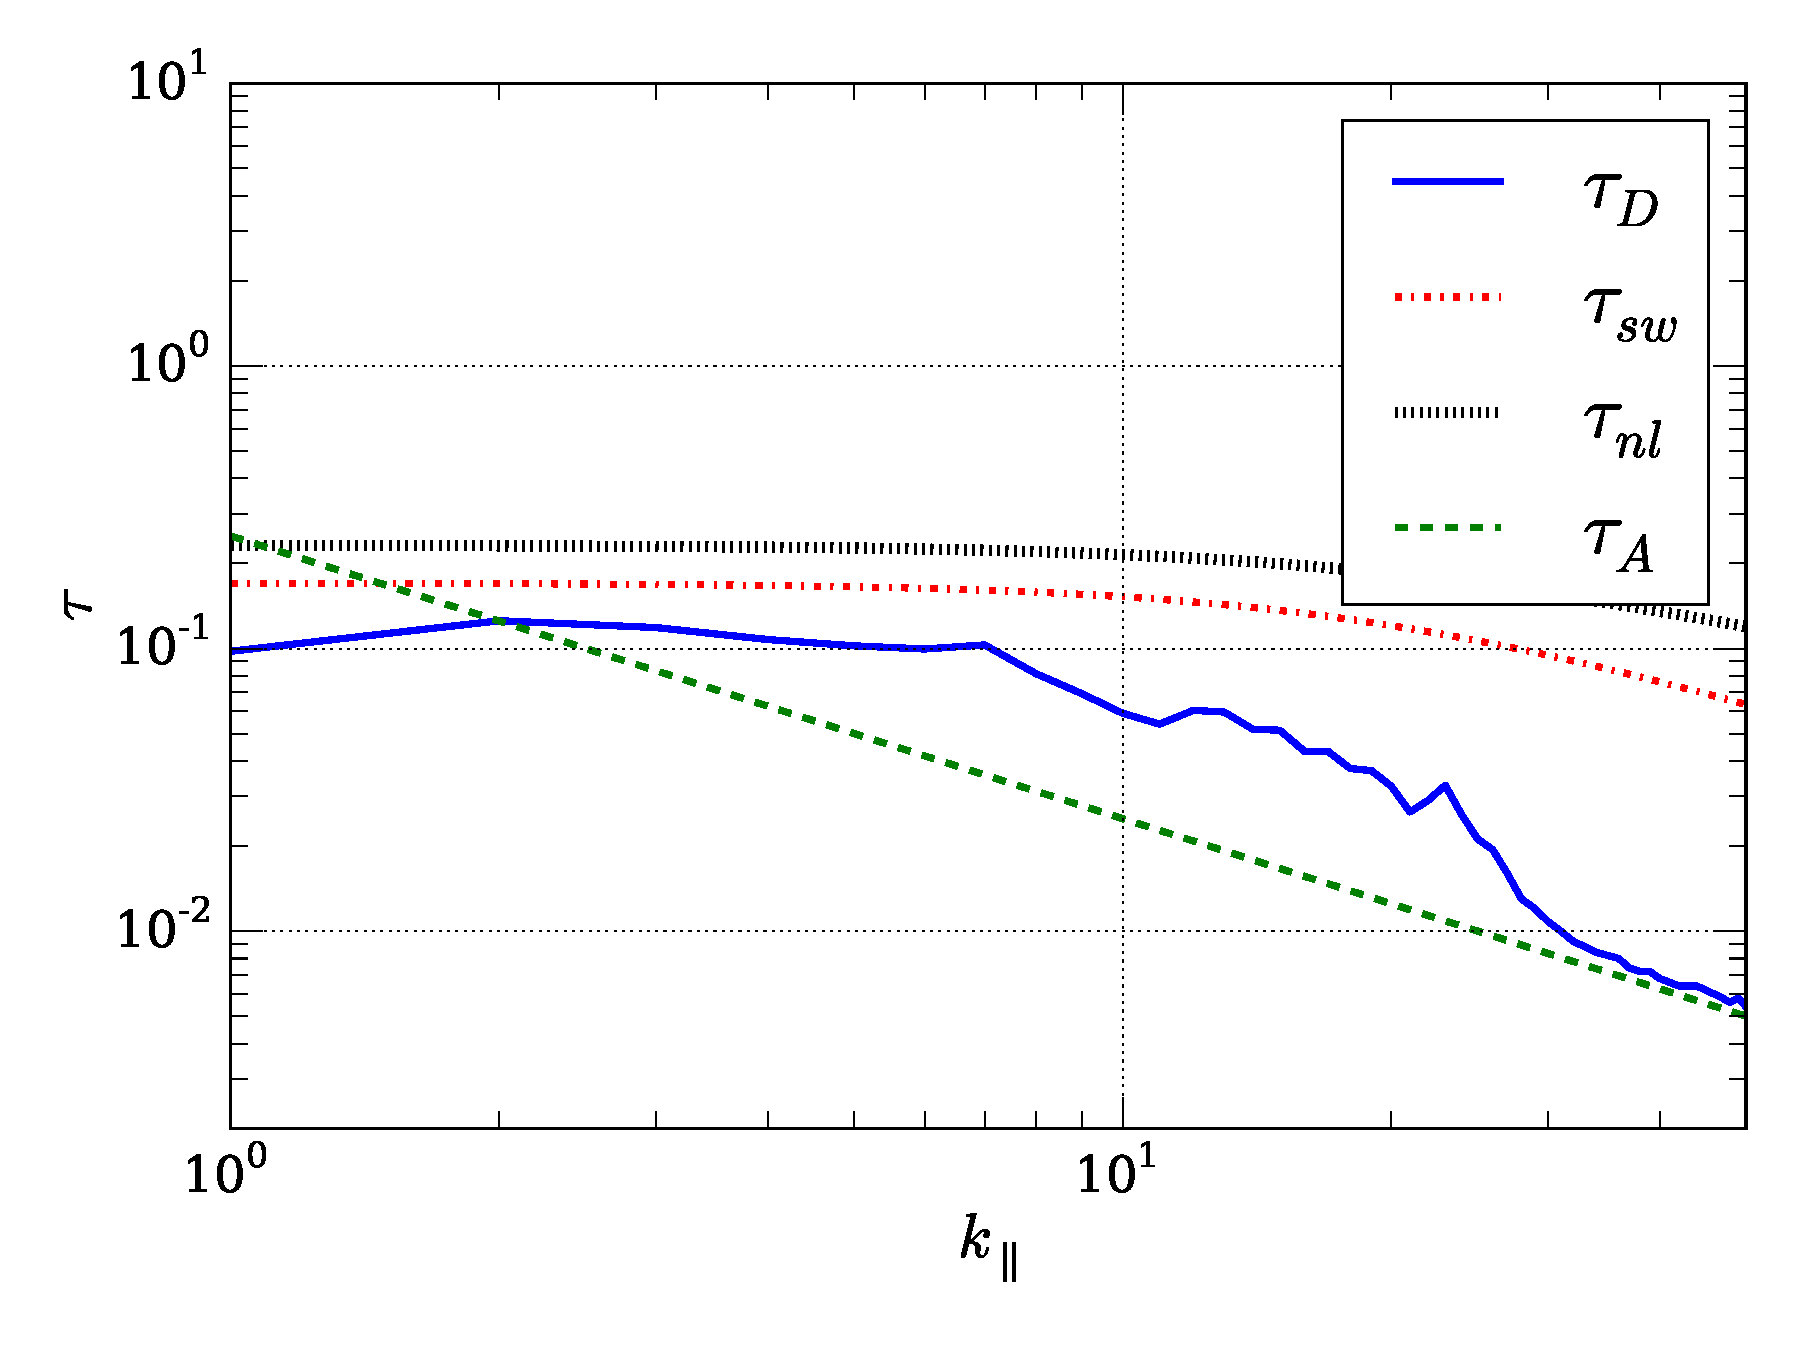
\includegraphics[width=1\columnwidth]{SpatioTemporalSpectra/fig5_B8_b_kperp_20-eps-converted-to.pdf}}
  \caption{Decorrelation times $\tau_D$ for the run with $B_0=8$. In each
    panel $k_\perp$ is held constant and $k_\parallel$ is varied; (a)
    $k_\perp=0$, (b) $k_\perp = 10$, and (c) $k_\perp = 20$. The
    straight lines indicate theoretical predictions for
    the scaling of the relevant physical time scales. In this case the
    Alfv\'en time controls the decorrelation at multiple wavenumbers.}
  \label{fig5:B8_bvf_b_kperp}
\end{figure}

\begin{figure}
  \centering
  \subfigure[$k_\parallel=0$]{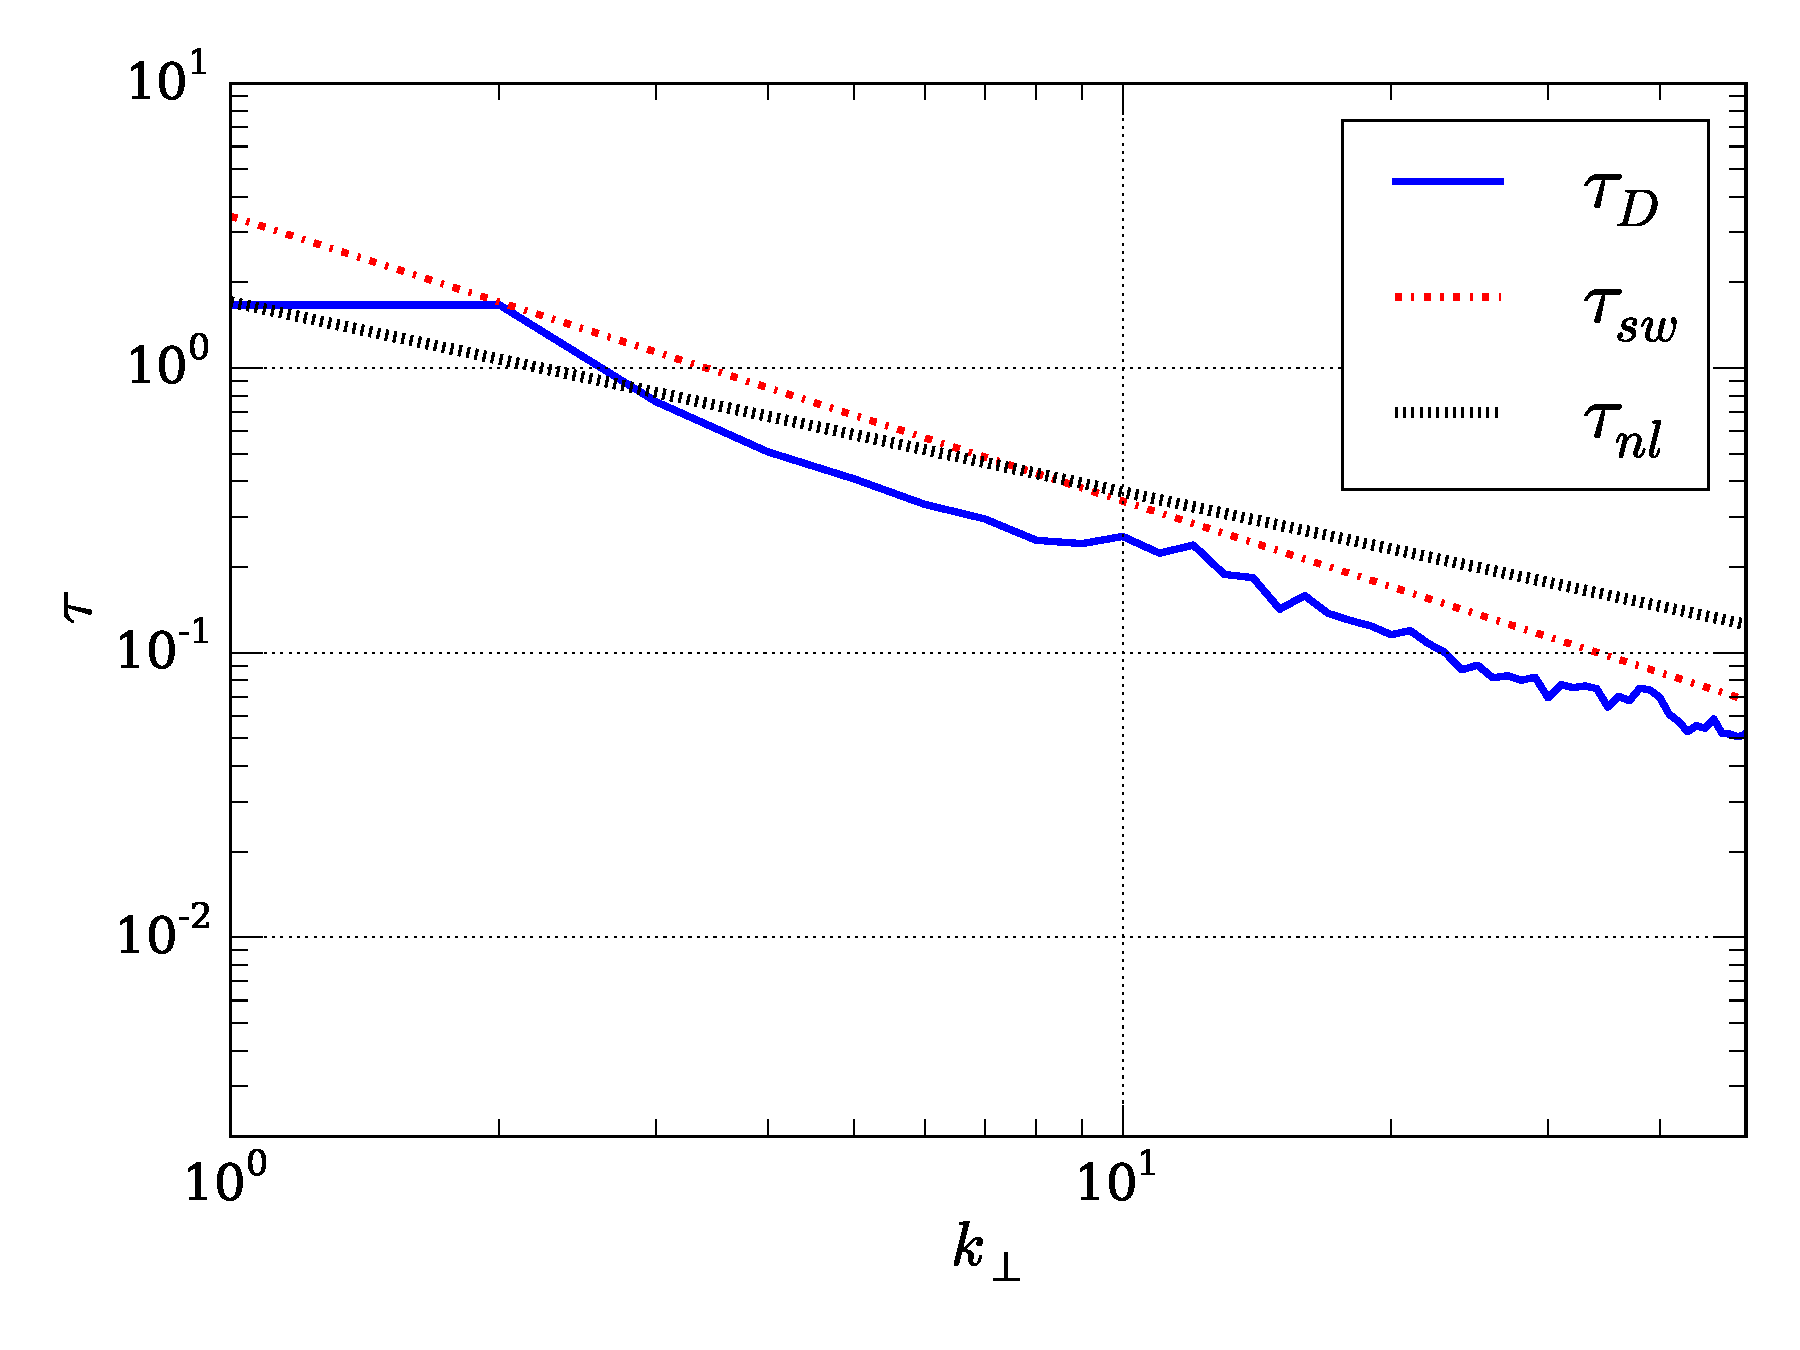
\includegraphics[width=1\columnwidth]{SpatioTemporalSpectra/fig5_B8_b_kpara_0-eps-converted-to.pdf}}

  \subfigure[$k_\parallel=10$]{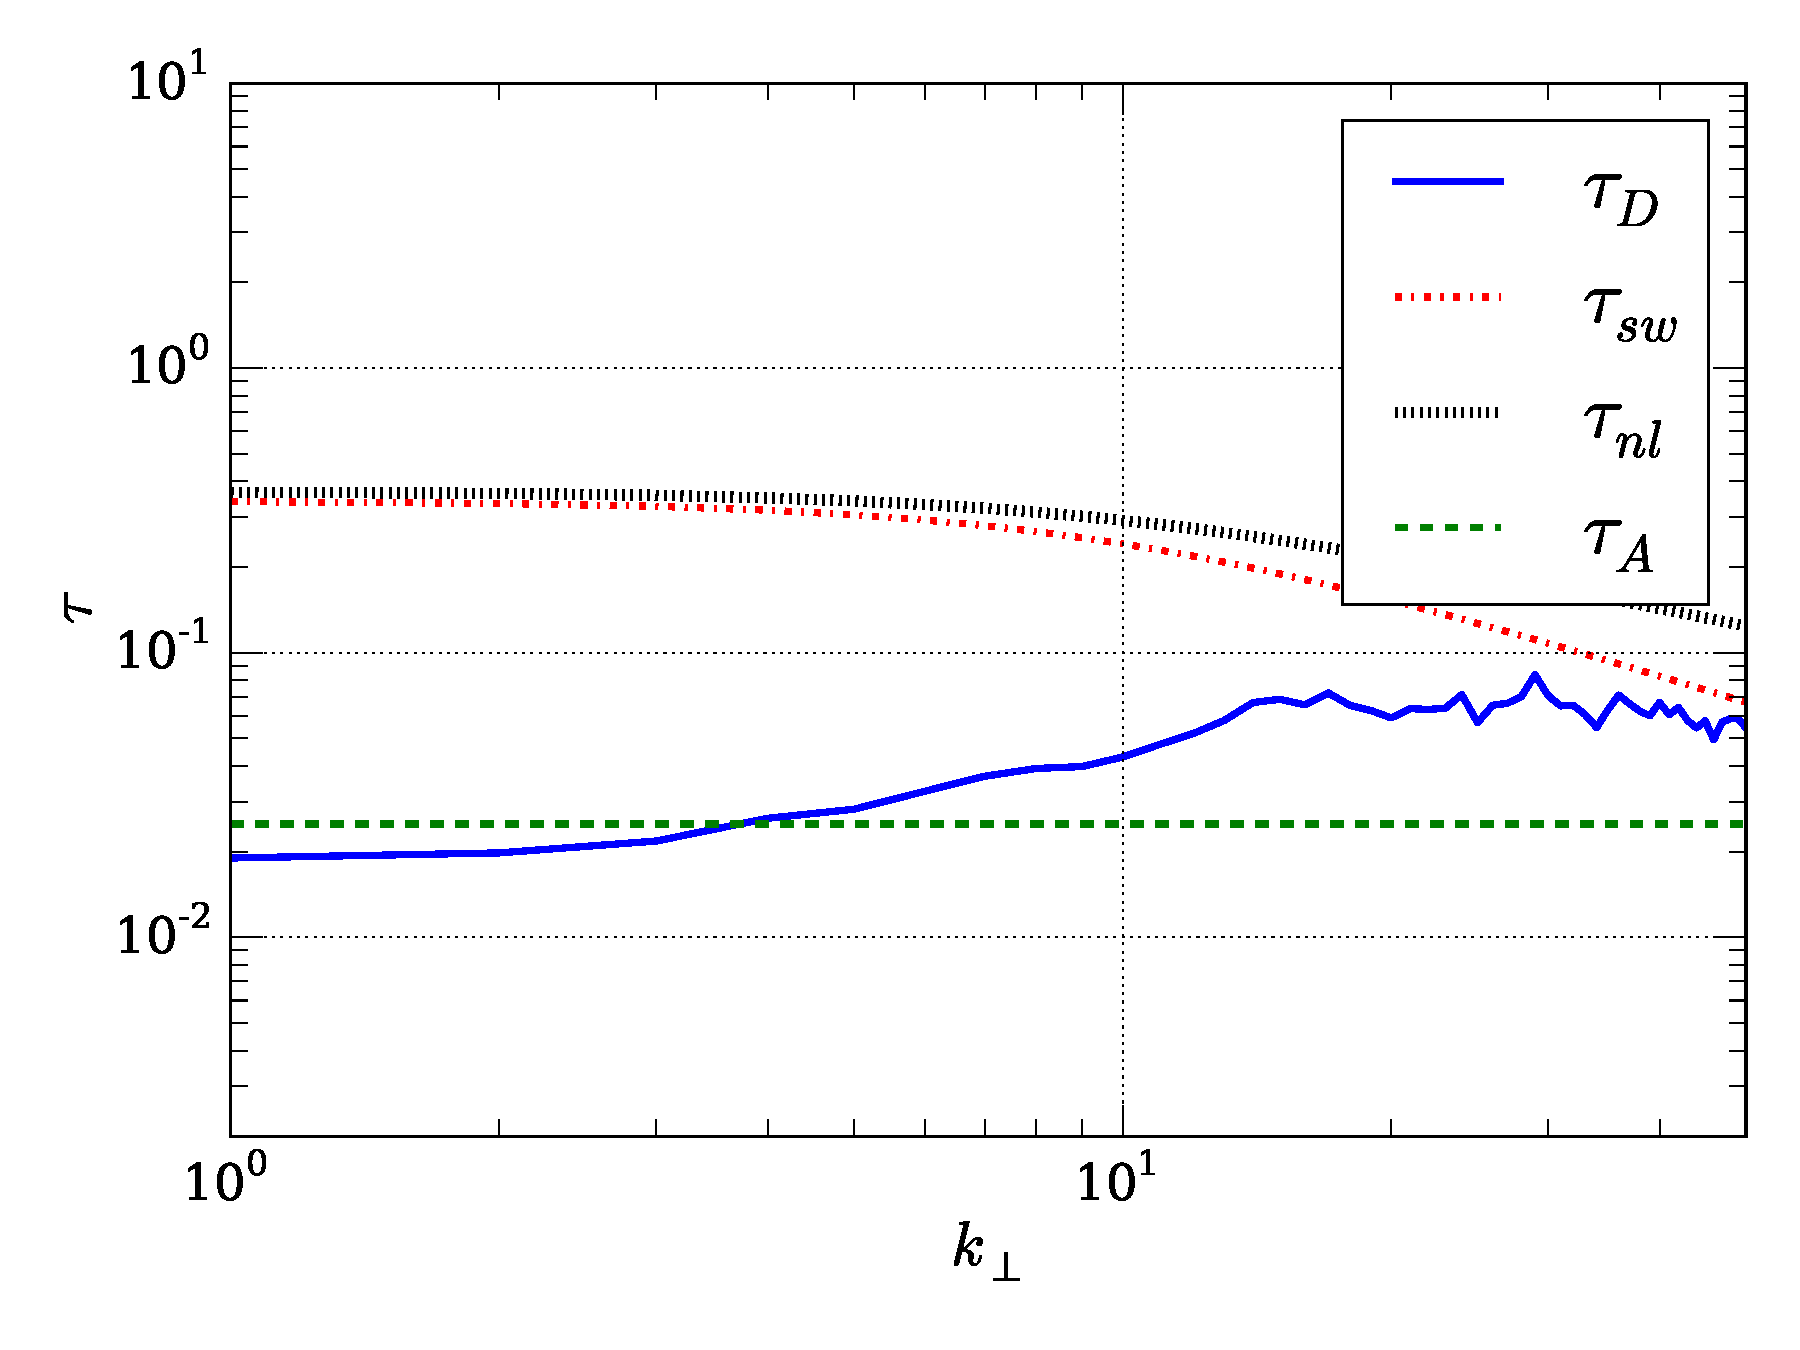
\includegraphics[width=1\columnwidth]{SpatioTemporalSpectra/fig5_B8_b_kpara_10-eps-converted-to.pdf}}

  \subfigure[$k_\parallel=20$]{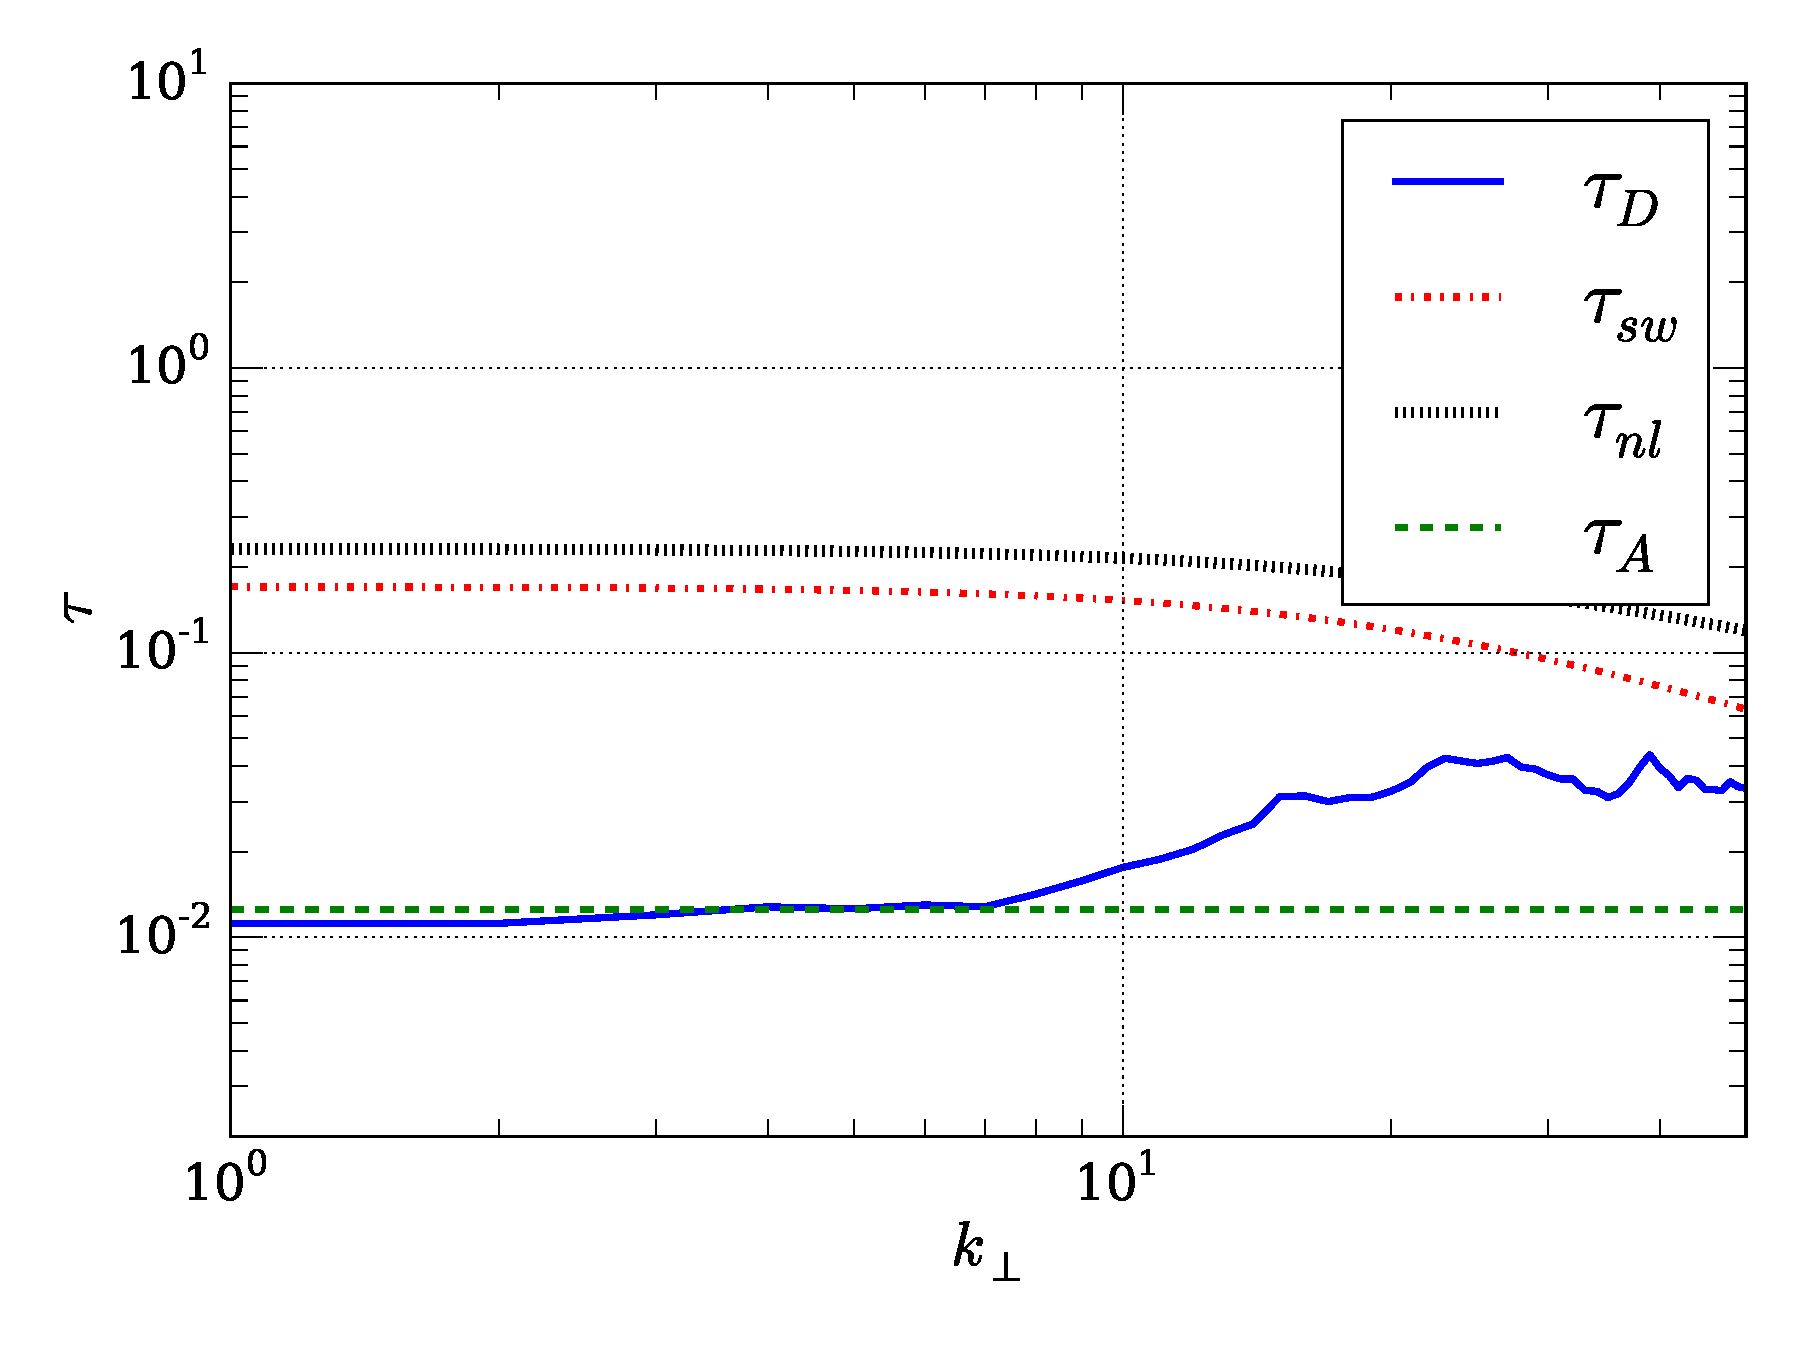
\includegraphics[width=1\columnwidth]{SpatioTemporalSpectra/fig5_B8_b_kpara_20-eps-converted-to.pdf}}
  \caption{Decorrelation times $\tau_D$ for the run with $B_0=8$. In each
    panel $k_\parallel$ is held constant and $k_\perp$ is varied; (a)
    $k_\parallel = 0$, (b) $k_\parallel = 10$, and (c) $k_\parallel =
    20$. The straight lines indicate theoretical predictions for
    the scaling of the relevant physical time scales. The Alfv\'en
    time controls the decorrelation up to $k_\parallel \approx 10$.}
  \label{fig5:B8_bvf_b_kpara}
\end{figure}


%%%%%%%%%%%%%%%%%%%%%%%%%%%%%%%%%%%%%%%%5
\section{Conclusions}\label{sec_Conclusions}

En este trabajo, hemos estudiado los tiempos de correlación que entran
en juego en magnetohidrodinámica, en la aproximación
incompresible. Aún en el caso (más simple) hidrodinámico, uno espera
que tanto las correalciones espaciales como las temporales sean
relevantes en la física de la turbulencia, ya que estas propiedades
independientes puede encarnarse en el tensor de correlación de dos
puntos y dos tiempos, $R_{ij}(\vec{r},t)$, una generalización directa
de la \cref{eq:Rbij}. Correlaciones análogas pueden ser escritas para
las componentes de la velocidad del fluido $\vec{u}$ y para otras
cantidades.  La transformada espacial de la correlación (o,
equivalentemente, las funciones de estructura espacial de segundo
orden) a tiempo de retraso $\tau$ nulo, proveen información acerca de
la distribución espacial de la energía a lo largo de las distintas
escalas. Acordemente, {\color{red}the zero spatial lag correlation,
  evaluated at varying time and transformed to frequency}, provee
información análoga acerca de la distribución energética a lo largo de
las distintas escalas temporales. Aquí, estudiamos las correlaciones
en tiempo para un dado número de onda o una escala espacial para el
modelo magnetohidrodinámico.

El caso MHD es más complejo que el hidrodinámico porque hay dos campos
involucrados: el magnético y el de velocidades. Además, el campo
magnético no puede ser removido por una transformada de Galileo,
mientras que el de velocidades, sí.  En consecuencia, el campo
magnético medio, impone una dirección preferencial. Adicionalmente, el
caso MHD tiene un nuevo y anisotrópico modo de ondas, las ondas de
Alfvén, que introducen la posibilidad de anisotropías en el espectro y
en las correlaciones, así como también una nueva escala temporal, el
tiempo de Alfvén. Debido a estos efectos, el análisis de la
descorrelación temporal se vuelve también más complejo, con al menos
tres escalas temporales para examinar (Alfvén, \sweeping y no lineal),
así como también la posibilidad de una anisotropía en la tasa de
descorrelación.

Tanto el \sweeping aleatorio como la correlación Alfvénica son efectos
no locales, en el sentido de que acoplan las grandes escalas con otras
más pequeñas. Los resultados mostrados aquí respaldan la conclusión de
que los efectos no locales (en el espacio espectral) juegan un rol
importante en turbulencia MHD (en acuerdo con los estudios de
transferencia \textit{shell-to-shell} \cite{alexakis_turbulent_2007,
  alexakis_anisotropic_2007, teaca_energy_2009, mininni_scale_2011}),
y que las descorrelaciones están principalmente dominadas por el
\sweeping y las interacciones Alfvénicas, confirmado los estudios
previos de MHD isotrópico \cite{servidio_time_2011}.

Además, en comparación con los estudios previos, el análisis aquí
presentado permite distinguir entre los efectos de \sweeping and
Alfvénicos, y los resultados apoyan la conclusión de que la
interacción de \sweeping domina la decorrelación para valores
moderados de $B_0$, mientras que para grandes valores del campo medio
$B_0$ y a grandes escalas (números de onda perpendiculares pequeños)
las descorrelaciones están más controladas por las interacciones
Alfvénicas.  Las interacciones relevantes son las ondas de Alfvén, y
como tales se puede concluir que las ondas se encuentran todavía
presentes en turbulencia MHD y dominan las descorrelaciones
esencialemnte para números de onda paralelos (alineados con el campo
medio; ver también \cite{meyrand_direct_2016,
  meyrand_weak_2015}). Nuestros resultados también indican que el
sistema elige, en efecto, el tiempo de descorrelación más bajo
disponible. Un constructo simple y relevante es que la tasa de
descorrelación es la suman de las tasas asociadas con cada escala de
tiempo relevante (ver, por ejemplo, \cite{pouquet_strong_1976,
  zhou_magnetohydrodynamic_2004}). Como resultado, aún para grandes
valores del campo guía $B_0$, para escalas suficientemente pequeñas en
las que el tiempo de \sweeping resulte más rápido que el de Alfvén,
luego de un gran rango de escalas en las que dominen las ondas de
Alfvéen, el sistema transiciona a un comportamiento donde domina el
\sweeping.


Una conclusión convincente del presente trabajo es que la influencia
de la descorrelación de \sweeping se extiende a lo largo de un amplio
rango de los parámetros globales. Aún si el \sweeping no es el tiempo
dominante de los mecanismos de descorrelación a lo largo de todo el
sistema, su importancia relatica a la descorrelación vía propagación
Alfvénica pensiste en ciertas subregiones del espacio de Fourier.
Este es el caso para valores moderados del campo magnético medio
aplicado $B_0$, como puede observarse en las
\cref{fig5:B1_bvf_b_kperp, fig5:B1_bvf_b_kpara}. Esta influencia del
\sweeping se encuentra aún en los casos con campo magnético medio
fuerte ($B_0 = 8$), como se ve en las \cref{fig5:B8_bvf_b_kperp,
  fig5:B8_bvf_b_kpara}. Acordemente, también se podría concluir que
los efecto de descorrelación Alfvénica son muy importantes, por lo
menos para valores altos de $B_0$ y en ciertas regiones del espacio de
ondas.  A pesar de que resulta difícil extrapolar tales conclusiones
en una forma precisa para aplicaciones espaciales y astrofísicas,
podemos aplicar los presentes resultados en una forma cualitativa.
Por ejemplo, el viento solar típicamente admite $\delta B/B_0 \sim 1$
en la escala más externa.  Aún si el cociente es menor, por ejemplo a
escalas menores en el rango inercial, el presente resultado sugiere
que el efecto de \sweeping se mantendría importante en establecer la
tasa del tiempo de descorrelación en el ambiente interplanetario. Esto
podría conllevar diversas implicaciones, por ejemplo en la predicción
cuantitativa, en la dispersión de partículas y en la comprensión del
ámbito de aplicación de la teoría de la turbulencia débil. En este
sentido, las técnicas de observación han comenzado a extraer medidas
aproximadas del viento solar y la descorrelación del tiempo
magnetosférico en el marco del plasma
\cite{matthaeus_ensemble_2016,weygand_magnetic_2013}, pero aún no han
alcanzado la precisión para distinguir los efectos de barrido y
Alfvénicos como lo ha hecho el presente estudio utilizando la
simulación MHD.

Es interesante recordar que la descorrelación de tiempo relevante
asociada con la transferencia de energía en turbulencia no es la
correlación de tiempo euleriana que hemos considerado (punto espacial
fijo, tiempo variable), sino más bien la descorrelación de tiempo
lagrangiana, calculada siguiendo un elemento fluido material. A este
respecto, es bien sabido que ni el barrido ni la propagación de ondas
alfvénicas pueden producir directamente la transferencia espectral en
modelos homogéneos idealizados. En parte debido a estas
complicaciones, actualmente no existe una teoría completa que vincule
la correlación espacial y las correlaciones de tiempo en MHD o
turbulencia hidrodinámica. Por otro lado, está claro que en MHD, tanto
la propagación de la onda de Alfvén como el \sweeping contribuyen a la
variación de tiempo total en un punto (espectro de frecuencia
euleriano) y, por lo tanto, influyen en una predicción
limitante. Estas escalas de tiempo también son características
importantes para comprender la dispersión de partículas de prueba
cargadas, como los rayos cósmicos de baja energía
\cite{bieber_proton_1994}, así como para tener en cuenta la
distribución de las aceleraciones, que está relacionada con la
intermitencia \cite{nelkin_time_1990}.

El comportamiento observado del tiempo de descorrelación para MHD,
ejemplificado por los nuevos resultados presentados aquí, tiene
aplicaciones en una serie de temas, incluyendo la teoría de dispersión
de partículas cargadas \cite{schlickeiser_cosmic-ray_1993,
  nelkin_time_1990}, la dinámica del campo magnético interplanetario y
de la magnetosfera \cite{miller_critical_1997}, y la interpretación de
datos de naves espaciales de misiones históricas y futuras
\cite{matthaeus_ensemble_2016}. Mirando hacia las perspectivas
futuras, notamos que ha habido cierto éxito en el establecimiento de
conexiones empíricas entre la escala de tiempo de \sweeping y la
descorrelación del tiempo euleriano observado en hidrodinámica
\cite{chen_sweeping_1989}. Se podrían aprovechar ideas similares para
MHD (por ejemplo, \cite{matthaeus_dynamical_1999}) para comprender
mejor, o al menos modelar empíricamente, la relación en MHD entre la
estructura espacial y la decorrelación del tiempo, un esfuerzo que se
beneficiaría directamente de los resultados novedosos presentados
aquí.
